\documentclass{article} % JASA requires 12 pt font for manuscripts
%\usepackage{JASA_manu}        % For JASA manuscript formatting

% for citations
\usepackage[authoryear]{natbib} % natbib required for JASA
\usepackage[colorlinks=true, citecolor=blue, linkcolor=blue]{hyperref}

%\definecolor{Blue}{rgb}{0,0,0.5}

\usepackage{amsthm}

% for figures
\usepackage{graphicx}
\usepackage{caption}
\usepackage{subcaption}
\graphicspath{{figures/}}
\newcommand{\hh}[1]{{\color{orange} #1}}
\newcommand{\al}[1]{{\color{red} #1}}

% color in tables
\usepackage{color}
\usepackage{colorbl}

% help with editing and coauthoring
\usepackage{todonotes}

% title formatting
\usepackage[compact,small]{titlesec} 
% page formatting
\usepackage[margin = 1in]{geometry}
\usepackage[parfill]{parskip}

% line spacing
\usepackage{setspace}
%\doublespace

% For math typsetting
\usepackage{bm}
\usepackage{amstext}
\usepackage{amssymb}
\usepackage{amsmath}
\usepackage{amsfonts}
\usepackage{multirow}
\usepackage{lipsum}

\newtheorem{theorem}{Theorem}
\newtheorem{definition}{Definition}

% A few commands to make typing less tedious
\newcommand{\inv}{\ensuremath{^{-1}}}
\newcommand{\ginv}{\ensuremath{^{-}}}
\newcommand{\trans}{\ensuremath{^\prime}}
\newcommand{\E}{\ensuremath{\mathrm{E}}}
\newcommand{\var}{\ensuremath{\mathrm{Var}}}
\newcommand{\cov}{\ensuremath{\mathrm{Cov}}}
\DeclareMathOperator{\tr}{Trace}

\title{Are you Normal? \\ {\Large The problem of confounded residual structures in hierarchical models}}
\author{
	Adam Loy and Heike Hofmann\\
	Department of Statistics,
	Iowa State University
}

\begin{document}
\maketitle

%----------------------------------------------------------------------------------
% Abstract

\begin{abstract}
We encounter hierarchical data structures in a wide range of applications. Regular linear models are extended by random effects to address correlation between observations in the same group. Inference for random effects is sensitive to  distributional mis-specifications of the model, making checks for (distributional) assumptions particularly important.  The investigation of residual structures is complicated by the presence of  different levels and corresponding  dependencies. Ignoring these dependencies leads to  erroneous conclusions using our familiar tools, such as Q-Q plots or normal tests. We first show the extent of the problem, then we introduce the {\it fraction of confounding} as a measure of the level of confounding in a model and finally introduce minimally confounded residuals as a solution to assessing distributional model assumptions.
\end{abstract}

%----------------------------------------------------------------------------------

%----------------------------------------------------------------------------------
\section{Introduction}\label{sec:intro}
%----------------------------------------------------------------------------------
There is a wide range of application areas---from the biological and physical sciences to the social sciences---in which we encounter nested  data.
Whether it is quality control in a manufacturing process that involves the monitoring of a set of components over  time  or students' performances in different schools across the country, analysts have to account for  the correlation between observations in the same group.  Hierarchical linear models \al{(i.e., mutlilevel models, linear mixed effects models)} allow us to do exactly that---but they also require us to make distributional assumptions on both the error terms and the random effects. These assumptions must hold to ensure the validity of the model. \todo{Do we need some transition here?} 
Inference for the fixed effects in linear mixed models is fairly robust against model mis-specification \citep{Butler:1992tx, Verbeke:1997tf}. This is different for random effects: they are sensitive to  distributional mis-specifications and  therefore have to be checked carefully\al{, especially when they are central to the inferential goals, such as in the construction of a prediction interval for an unobserved group}.

Quantile-quantile (Q-Q) plots \citep{Wilk:1968} are our main graphical tool for evaluating a specific distributional assumption. For that, we plot the empirical distribution against \al{the} expected quantiles \al{from the assumed distribution}. In hierarchical \al{linear} models the investigation of residual structures is complicated by the presence of  different levels. 
The nested structure of the data is reflected in the residual structure, and just as there is dependence between different levels in the data, we can expect dependencies between different levels in the residual structure. Q-Q plots, \al{in their} weighted \citep{Dempster:1985tr, Lange:1989uu} or unweighted \al{form}, do not account for this, which can lead us to erroneous conclusions in evaluating normality based on the plots (or any other \al{standard} test).

% however, these plots, weighted or unweighted, do not account for the relationship between the predicted random effects and error terms and result in inflated type I error rates. 

%From a graphical perspective the assessment of the assumptions made on the random effects has focused on plotting the empirical distribution of the predicted random effects in quantile plots 

In this paper, we address the problem of distributional assessment due to confounding in residual structures. 
First, we illustrate the inadequacy of existing methods  based on the predicted residuals. 
We then introduce  the concept of least confounded \todo{I might like `rotated' more} residuals for the random effects and present a general method to obtain least confounded residuals for residuals at all levels of the model. We demonstrate how this enables an appropriate (graphical) assessment  of distributional assumptions.
\todo[inline]{Return to this paragraph after more writing...}


\section{Motivating example}\label{sec:ex}
%To motivate our discussion
To illustrate the effect of confounding between different levels of residuals, we consider the data set presented by
 \cite{Gelman:2006ue}. This data set consists of a stratified random sample of 919 owner-occupied homes nested within 85 counties in Minnesota, for which the authors suggested a hierarchical model of the form
%
\begin{equation}\label{eq:radon}
  \log(y_{ij}) = \beta_0 + \beta_1 x_{1ij} + \beta_2 x_{2i} + b_{0i} + b_{1i} x_{1ij}  + \varepsilon_{ij}
\end{equation}
%
where   $\log(y_{ij})$ denotes the (log pCi/L, i.e log picoCurie per litre) radon measurement for house~$j$ ($1 \le j \le n_i, 1 \le i \le 85$) within county~$i$,
 $x_{1ij}$ is a binary variable describing the level at which the measurement was taken (0 for the basement and 1 for a higher level) and $x_{2i}$ denotes the average soil uranium content for  county~$i$. 
 Further, we assume i.i.d. normal errors $\varepsilon_{ij} \sim \mathcal{N} (0,\ \sigma^2_{\varepsilon})$  and $\bm{b}_i \sim \mathcal{N}(\bm{0},\ \bm{D})$, where $\bm{D}$ allows for correlation between $b_{0i}$ and $b_{1i}$. We also assume independence between random effects and error \al{terms}. 


A map of counties in Minnesota is given in figure \ref{fig:map}. The color shading represents average radon activity in a county. For two counties no data is available. Generally, more southern locations exhibit higher  levels of Radon activity. Figure \ref{fig:tc} focuses on the two counties of Hennepin (home to Minneapolis) and Winona (home to the city of the same name). Radon levels are plotted by floor level. Radon levels are usually the highest at the basement level of a house. 
%
\begin{figure}[htb]
\centering
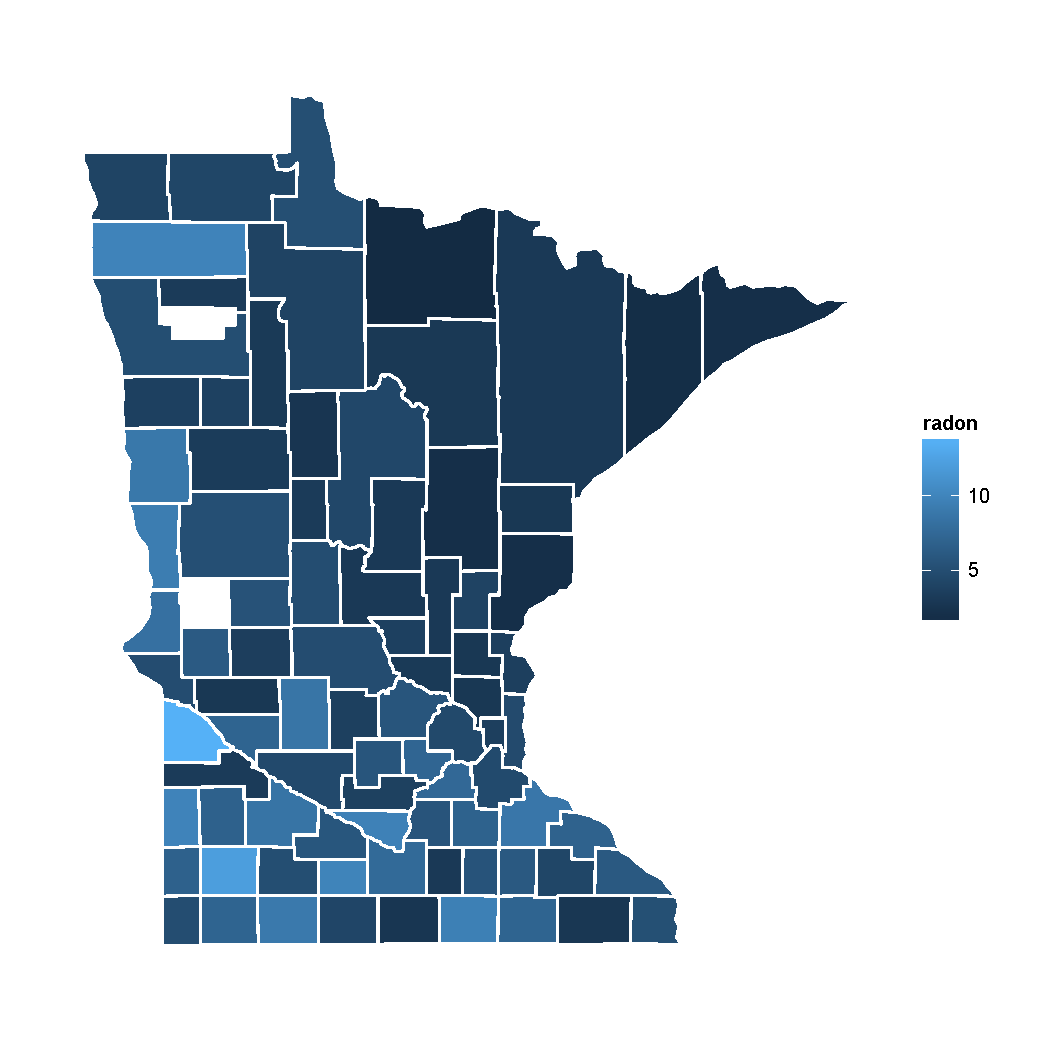
\includegraphics[width=0.5\linewidth]{figures/map.pdf}
\caption{\label{fig:map} Map of the counties in Minnesota. The color shading represents average Radon activity.}
\end{figure}
%
\begin{figure}[htb]
\centering
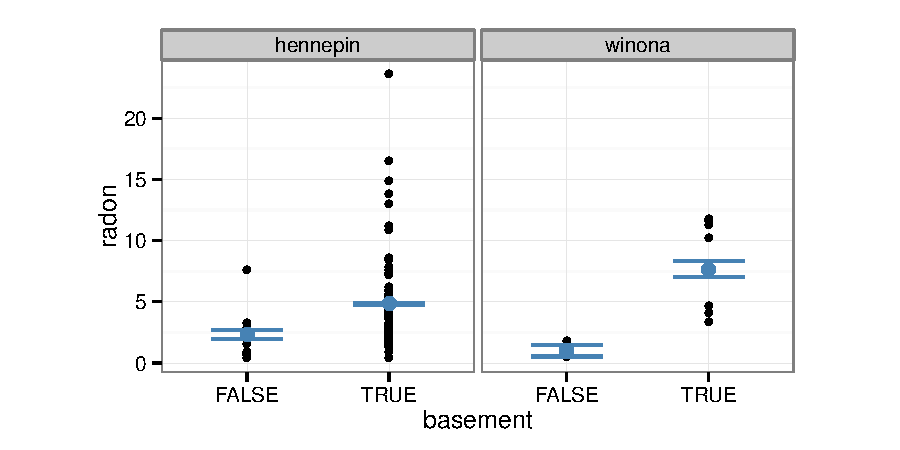
\includegraphics[width=0.7\linewidth]{figures/radon-twocounties.pdf}
\caption{\label{fig:tc} Activity of radon levels for the two counties of Hennepin and Winona at basement levels and higher. Radon levels at the basement level are usually higher.}
\end{figure}
%
The within-county sample sizes, $n_i$, are extremely unbalanced, ranging from one house to 116 houses, with 50\% of the counties having between three and ten houses. Such unbalanced designs are common in applications, and result in a high degree of pooling \al{(shrinkage)} for the predicted county-level random effects. % \citep[see][figure 3]{Gelman:2006ue}. 
This leads to dependence between  predicted random effects and  error terms (cf. eqns. \ref{eq:resid1} and \ref{eq:resid2}), which in turn can lead us to draw erroneous conclusions for corresponding residual quantities.


\begin{figure}[htb]
	\centering
	  \begin{subfigure}[b]{0.3\linewidth}
		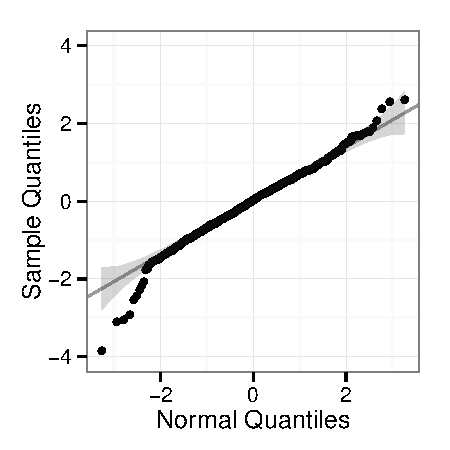
\includegraphics[width=\linewidth]{raw-lev1-qq.pdf}
		\caption{Predicted error terms}
	  \end{subfigure}	
	  \begin{subfigure}[b]{0.3\linewidth}
	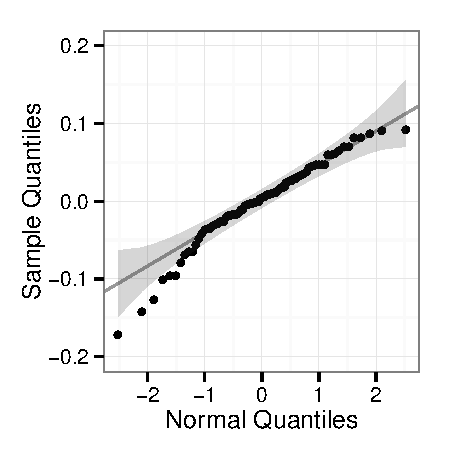
\includegraphics[width=\linewidth]{raw-intercept-qq.pdf}
		\caption{Random intercepts}
	  \end{subfigure}	
%	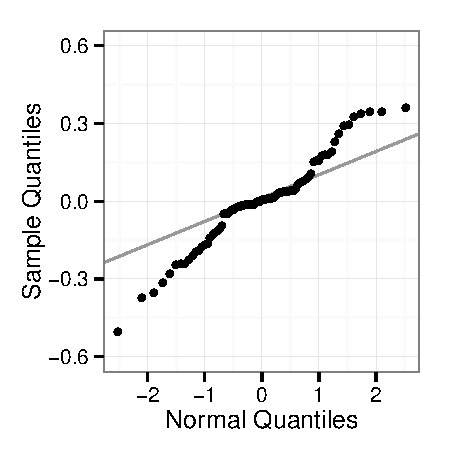
\includegraphics[width=0.32\textwidth]{raw-slope-qq.pdf}
	\caption{\label{fig:qqplots1} Q-Q plots of predict\al{ed residuals} at different levels %, and random slopes (right) 
	for model~\eqref{eq:radon}. Note that random slopes (not shown) exhibited the largest deviation from normality -- see figure~\ref{fig:lineup}. }
\end{figure}


\begin{figure}[htb]
	\centering
	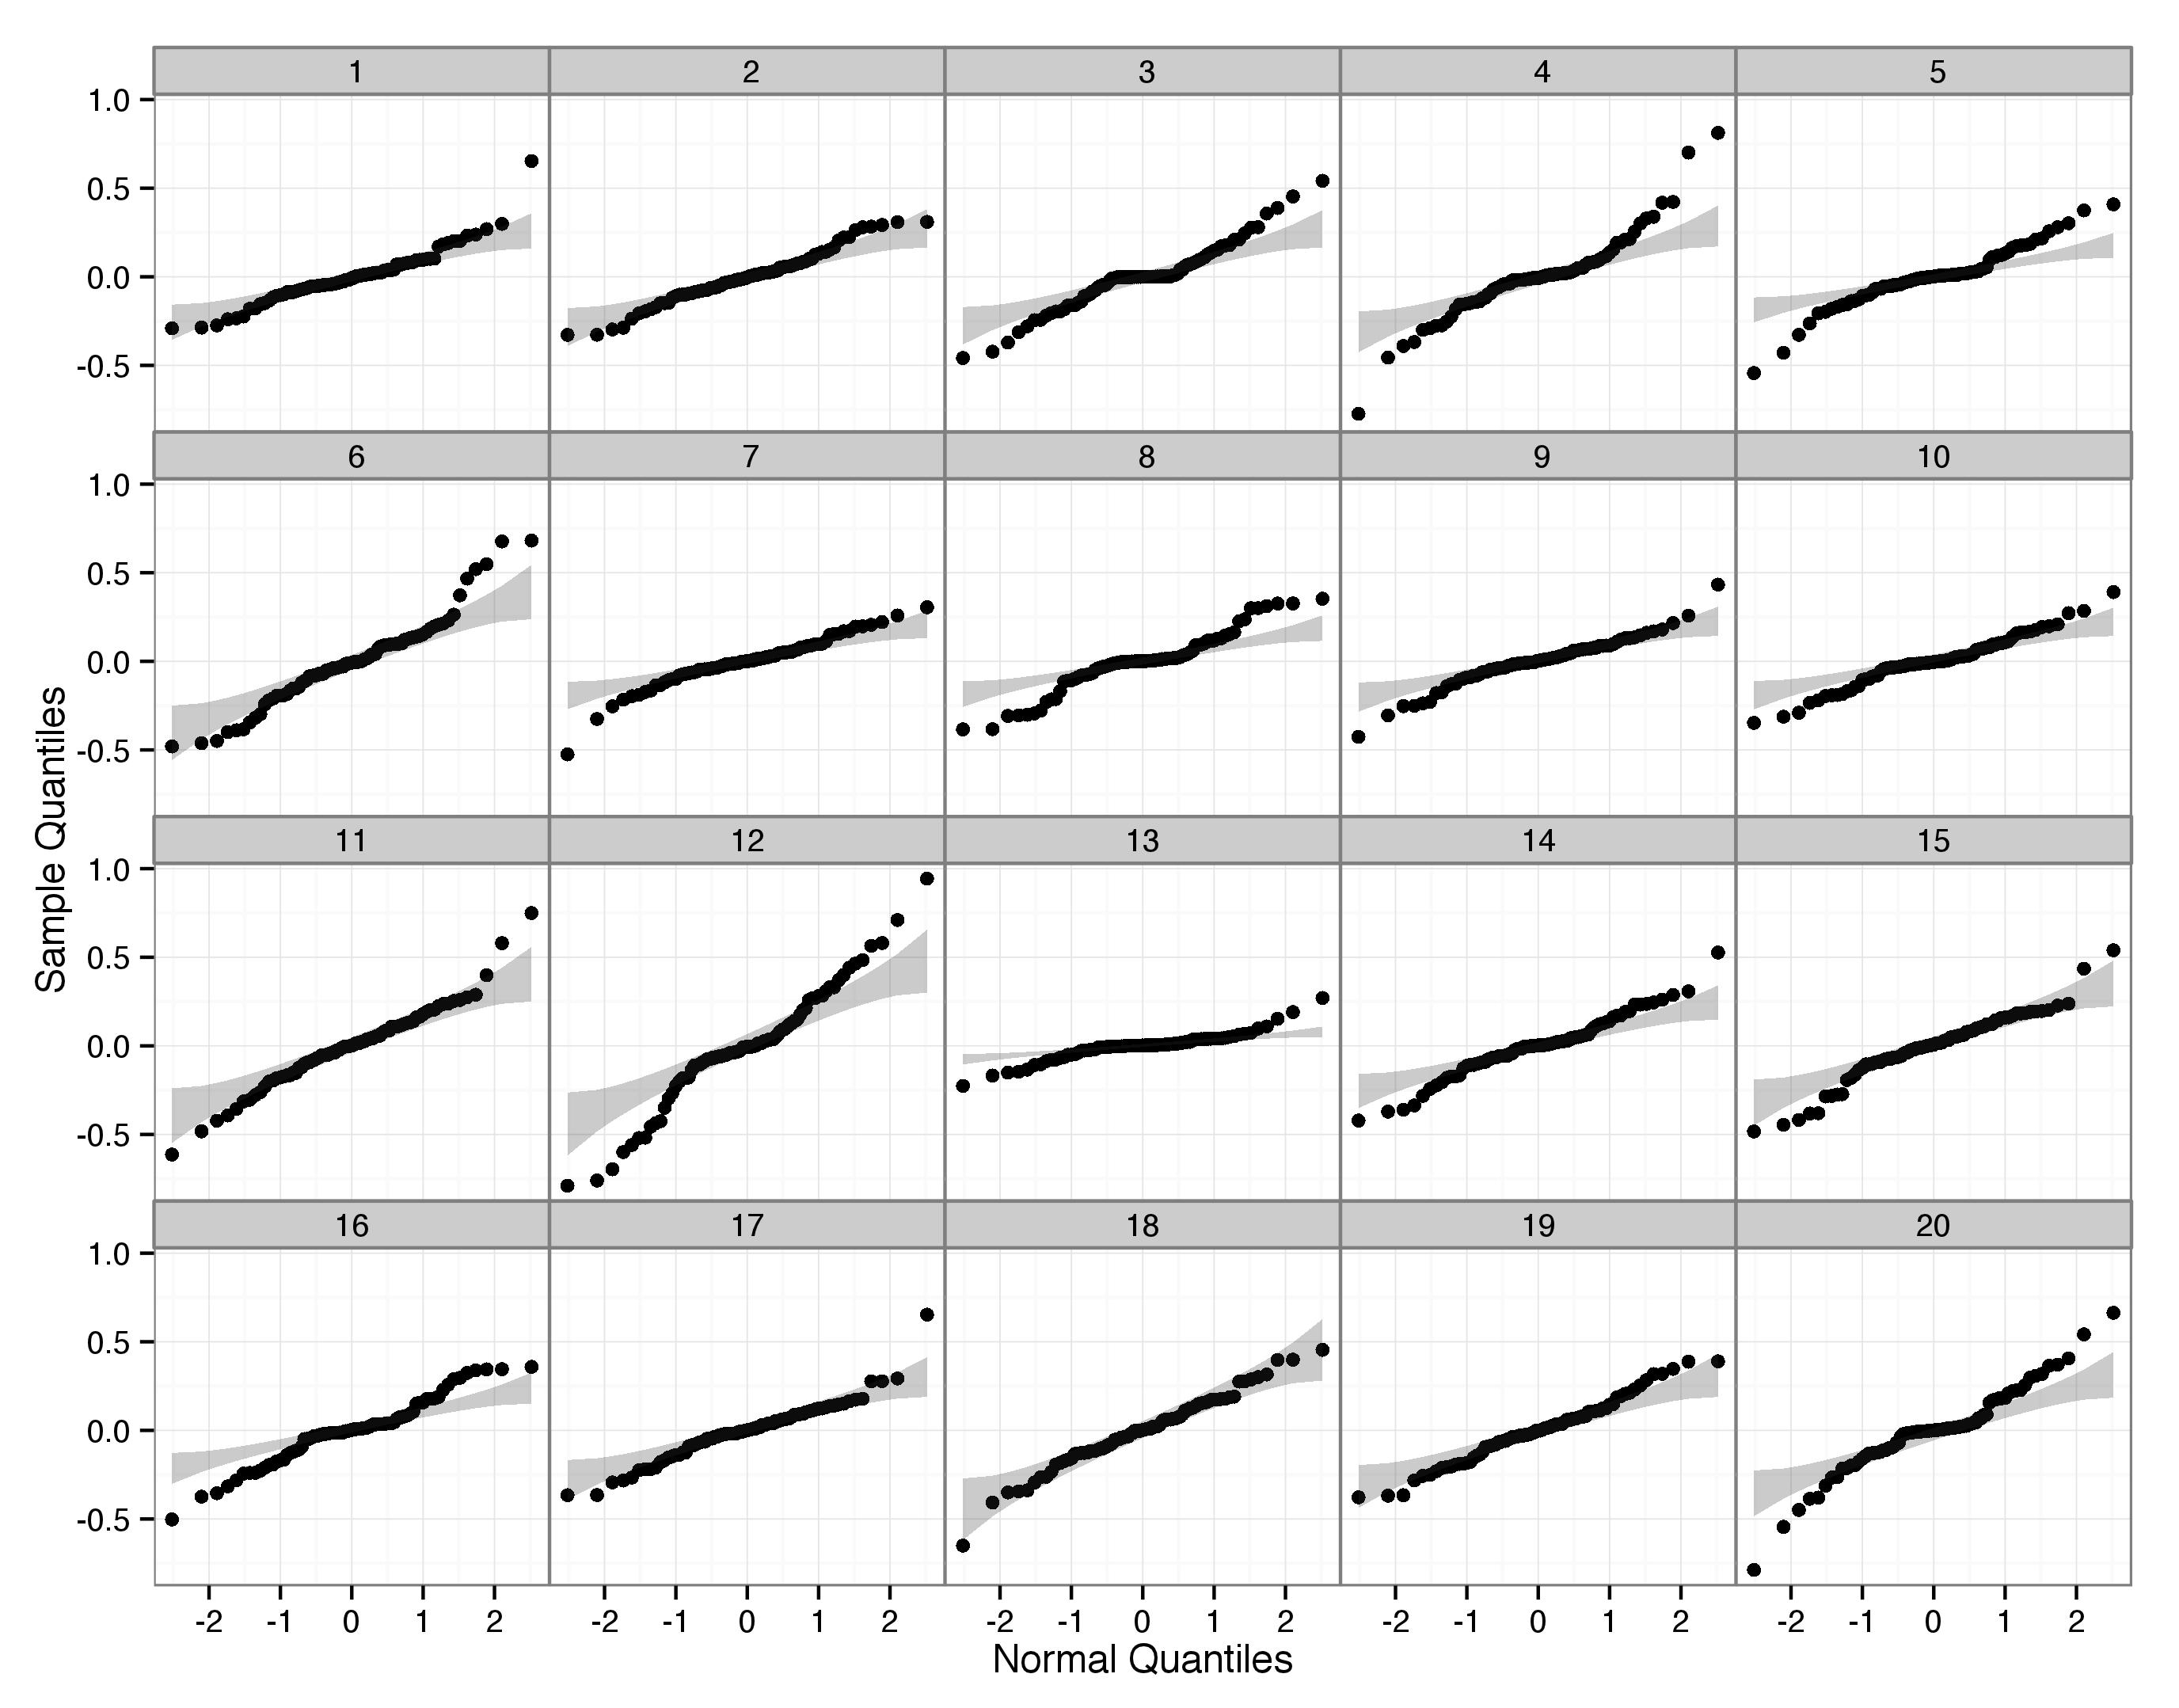
\includegraphics[width=0.9\textwidth]{test.jpeg}%lineup-rslope.pdf}
	\caption{\label{fig:lineup} Lineup of normal Q-Q plots for the random slope term in model~\eqref{eq:radon}. The 19 null plots were obtained by simulation from the model. Can you identify the observed Q-Q plot?}
\end{figure}

In this example, Q-Q plots (Figure~\ref{fig:qqplots1}) for the residuals show that normality 
seems to be violated 
for the error terms and both random effects. But is this cause for concern?
\al{Since} there is little pooling at the observation level \al{(level 1)} we expect the distributional assessment of the error terms to be reliable, but  for the random effects the high degree of pooling  casts doubt on the reliability of their Q-Q plots. 
We find our doubts increasing in a simulation-based assessment of distributions for residuals and random effects.

Figure~\ref{fig:lineup} shows a lineup \citep{buja:2009} of 20 Q-Q plots for the predicted random slope. The Q-Q plot of the observed random slopes is placed among nineteen decoy plots of parametric bootstrap samples based on model~\eqref{eq:radon} satisfying the normal distribution assumptions. The simulation parameters were set to the maximum likelihood estimates of model~\eqref{eq:radon}.
The observed Q-Q plot (panel $12+2^2$) is virtually indistinguishable from the field of null plots. This suggests that the predicted random slopes  from the data do not deviate significantly from model~\eqref{eq:radon}. 
%A lineup of the random intercepts revealed the same finding and was omitted for brevity. 
Note that in practice we must blind ourselves from the true plot for proper use of lineups. In order to not violate this, we did not show the Q-Q plot of random slopes earlier.
%
%application of the Anderson-Darling test results in the rejection of the null hypothesis of normality at the .05 significance level for the error terms and both random effects. As there is little pooling at the observation level we would expect the distributional assessment of the error terms to be reliable, but this is not the case with the random effects. 
%
%To further explore the distributional assumptions made on the random effects we create lineups \citep{buja:2009} of quantile plots were created by randomly inserting the true quantile plot for each term into a field of 19 plots generated under the null hypothesis of normality. A lineup for the random slopes is presented in Figure~\ref{fig:lineup}. The observed quantile plot (panel 16) is indistinguishable from the field of null plots, indicating that these predicted random slopes do not deviate from what would be expected under model~\eqref{eq:radon}, contradicting the results of the AD test. 

What becomes apparent from the lineup, is that, astonishingly, {\it none} of the null plots conforms to normality. Further investigation  revealed  that a  proportion far above the nominal 0.05 of distributions of random intercepts  fail the normality tests, too.


%Further evidence of the impact of this dependence is evident from a small scale simulation study. We used the design of the radon study to simulate 5000 data sets under model~\eqref{eq:radon} satisfying the assumptions discussed above. The simulation parameters were set to the maximum likelihood estimates of model~\eqref{eq:radon}. 
%%: $\widehat{\beta_0} = 1.46$, $\widehat{\beta_1} = -0.64$, $\widehat{\beta_2} = 0.77$, $\widehat{\sigma}_{\varepsilon} = 0.75$, $\widehat{\sigma}_{b_0} = 0.12$, $\widehat{\sigma}_{b_1} = 0.35$, and $\widehat{\rho} = 0.26$. 

Table~\ref{tab:edf} shows results from 1000 parametric bootstrap samples of model~\eqref{eq:radon} under normal errors.
For each simulated data set, we evaluated the assumption of normality for both the level-1 and -2 residuals using the Anderson-Darling (AD), Cram{\'e}r von Mises (CVM), and  Kolmogorov-Smirnov (KS), tests for normality.  
%Table~\ref{tab:edf} shows the proportions of the tests of the empirical distribution function rejecting the null hypothesis of normality at the .05 significance level. 
Type I error rates are hugely inflated for both random effects, making an assessment of normality based on the empirical distribution impossible.
%The inflated type I error rates for the random effects indicate that the empirical distribution of the random effects cannot be used to assess the assumption of normality. 
In the example we are able to use  the empirical distribution for assessing normality of  level-1 residuals  as  pooling is minimal at this level. In situations with higher levels of pooling, this may not be the case.

%For example, in Figure~\ref{fig:lineup} we present a lineup \citep{buja:2009} of 20 quantile plots for the predicted random slope, 19 of which were generated under the null hypothesis of normality. The observed quantile plot (panel $12+2^2$) is virtually indistinguishable from the field of null plots, indicating that these predicted random slopes do not deviate from what would be expected under model~\eqref{eq:radon}. A lineup of the random intercepts revealed the same finding and was omitted for brevity. 
%
%%An alternative approach would be the use of simultaneous simulation envelopes \todo{Is a citation needed here?}. 
%%
%%application of the Anderson-Darling test results in the rejection of the null hypothesis of normality at the .05 significance level for the error terms and both random effects. As there is little pooling at the observation level we would expect the distributional assessment of the error terms to be reliable, but this is not the case with the random effects. 
%%
%%To further explore the distributional assumptions made on the random effects we create lineups \citep{buja:2009} of quantile plots were created by randomly inserting the true quantile plot for each term into a field of 19 plots generated under the null hypothesis of normality. A lineup for the random slopes is presented in Figure~\ref{fig:lineup}. The observed quantile plot (panel 16) is indistinguishable from the field of null plots, indicating that these predicted random slopes do not deviate from what would be expected under model~\eqref{eq:radon}, contradicting the results of the AD test. 
%
%Further evidence of the impact of this dependence is evident from a small scale simulation study. We used the design of the radon study to simulate 1000 data sets under model~\eqref{eq:radon} satisfying the assumptions discussed above. The simulation parameters were set to the maximum likelihood estimates of model~\eqref{eq:radon}: $\widehat{\beta_0} = 1.46$, $\widehat{\beta_1} = -0.64$, $\widehat{\beta_2} = 0.77$, $\widehat{\sigma}_{\varepsilon} = 0.75$, $\widehat{\sigma}_{b_0} = 0.12$, $\widehat{\sigma}_{b_1} = 0.35$, and $\widehat{\rho} = 0.26$. For each simulated data set, we evaluated the assumption of normality for both the level-1 and -2 residuals using the Shapiro-Wilk (SW), Aderson-Darling (AD), Cram{\'e}r von Mises (CVM), and Kolmogorov-Smirnov (KS) tests for normality.  Table~\ref{tab:edf} shows the proportions of the tests of the empirical distribution function rejecting the null hypothesis of normality at the .05 significance level. The inflated type I error rates for the random effects indicate that the empirical distribution of the random effects cannot be used to assess the assumption of normality. In this situation, the empirical distribution of the level-1 residuals can be used to assess normality as minimal pooling is present at this level. In situations with higher levels of pooling, this will not be the case.
%

\begin{table}[!h]
\caption{\label{tab:edf} Proportions of tests rejecting the null hypothesis of normality of the predicted error terms and random effects at the nominal .05 significance level. Type I error rates are hugely inflated. \vspace{.5em}
}
\begin{center}
\begin{tabular}{l rrr} \hline
& \multicolumn{3}{c}{Test} \\ \cline{2-4}
 Residual &  AD & CVM & KS \\ \hline
Error term			 & 0.06 & 0.06 & 0.05\\
\rowcolor{gray!20} Random intercept 	& 0.48 & 0.46 & 0.35\\
\rowcolor{gray!20} Random slope 		& 0.75 & 0.75 & 0.68\\
   \hline
\end{tabular}
\end{center}
\end{table}

In the remainder of this paper we investigate the root of concern that leads to the distributional deviations, and derive residuals that address the issues introduced by pooling, allowing for a familiar graphical assessment of these distributions.


%----------------------------------------------------------------------------------
\section{Hierarchical linear models and residuals}\label{sec:resid}
%----------------------------------------------------------------------------------
The general stacked representation of the hierarchical linear model is given by
%
\begin{eqnarray}\label{eq:hlm}
 && \bm{y} = \bm{X \beta} + \bm{Z b} + \bm{\varepsilon}, \\ \nonumber
 && \E \begin{bmatrix} \bm{b} \\ \bm{\varepsilon} \end{bmatrix} = \bm{0}, 
 \ \cov \begin{bmatrix} \bm{b} \\ \bm{\varepsilon} \end{bmatrix} = 
  	\begin{bmatrix} \bm{D} & \bm{0}\\ \bm{0} & \bm{R} \end{bmatrix}
\end{eqnarray}
%
where $\bm{y}$ is an $n \times 1$ vector of observed responses, $\bm{X}$ ($n \times p$) and $\bm{Z}$ ($n \times q$) are design matrices, $\bm{\beta}$ is a $p \times 1$ vector of unknown fixed effects, $\bm{b}$ is a $q \times 1$ vector of unobserved random effects, $\bm{\varepsilon}$ is an $n \times 1$ vector of unobserved errors, and $\bm{R}$ and $\bm{D}$ are positive definite covariance matrices.

  %Additionally, it is often assumed that $\bm{\varepsilon}$ and $\bm{b}$ are normally distributed. 
Using this specification, the predicted error terms and random effects are given by 
%
\begin{align}
\widehat{\bm{\varepsilon}} &= \bm{RPy} = \bm{RPZb} + \bm{RP \varepsilon} \label{eq:resid1}\\
\widehat{\bm{b}} &= \bm{DZ}\trans \bm{Py} = \bm{DZ}\trans \bm{PZb} + \bm{DZ}\trans \bm{P \varepsilon} \label{eq:resid2}
\end{align}
%
where $\bm{P} = \bm{V}\inv( \bm{I} - \bm{X} (\bm{X}\trans \bm{V}\inv \bm{X})\inv \bm{X}\trans \bm{V}\inv)$. This  set of equations %\eqref{eq:resid1} and \eqref{eq:resid2} 
reveals the inherent dependence between the the residuals.
Additionally, it is easily seen that both \eqref{eq:resid1} and \eqref{eq:resid2} lead to the analysis of correlated and potentially heteroscedastic disturbances as $\var(\widehat{\bm{\varepsilon}}) = \bm{RPR}$ and $\var(\widehat{\bm{b}}) = \bm{DZ}\trans \bm{PZD}$.

\todo[inline]{Should we incorporate some discussion of the other simulations that I have run? If so I was thinking this section would be the place.}


%----------------------------------------------------------------------------------
\section{Rotating the random effects}\label{sec:rotate}
%----------------------------------------------------------------------------------

To combat the issues presented above, we derive a reduced set of minimally confounded residuals that are standardized, uncorrelated, and homoscedastic. \al{Our discussion focuses on the random effects, but it is straightforward to generalize the method to residuals at other levels.} \cite{HildenMinton:1995wh} presents the derivation of a similar set of minimally confounded residuals for the error terms, but did not address the random effects. The derivation is relegated to the appendix, and presents a more general method that applies to residuals at all levels of the model.

\al{
To assess the distributional assumptions made on the random effects we must evaluate the each random effect separately. To this end, when there is more than one random effect in a model we must define linear combinations $\bm{L}_k$ such that $\bm{L}_k\trans \widehat{\bm{b}}$ produces the $k$th random effect. For example, in the radon study described above, if $\bm{Z}$ is organized as a block diagonal matrix, that is $\bm{Z} = \bigoplus_{i=1}^{m} \bm{Z}_{i}$ where $\bigoplus$ denotes the direct sum \citep[page 47]{Gentle:2007}, then $\bm{L}_0 = \bm{I}_{85} \bigotimes ( 1,\ 0)$ produces the random intercepts and $\bm{L}_0 = \bm{I}_{85} \bigotimes ( 0,\ 1)$ produces the random slopes. In the following discussion we will present formulas using $\widehat{\bm{b}}$ as if there is only a single random effect in the model, but substitution of $\bm{L}_k\trans \widehat{\bm{b}}$ generalizes the expressions to more complicated models.

Next, we define the \emph{fraction of confounding} for the random effects, which is minimized in the result below. This definition generalizes the fraction of confounding proposed by \cite{HildenMinton:1995wh}.} \\

%\begin{definition}[Fraction of confounding]\label{def:fc1}
%For the $i$th element of the target residual vector, $\widehat{\bm{e}}$, the fraction of confounding is given by
%%
%\begin{equation}\label{eq:fc}
%	\text{FC}(\widehat{\bm{e}}_i) 
%	= \frac{\bm{v_i}\trans \var(\widehat{\bm{e}} | \bm{e}) \bm{v_i}}
%		{\bm{v_i}\trans \var(\widehat{\bm{e}}) \bm{v_i}}
%	= \frac{\bm{v_i}\trans \bm{A} \bm{v_i}}
%		{\bm{v_i}\trans \bm{B} \bm{v_i}}
%\end{equation}
%
%where $\bm{v_i}$ is the $i$th column of the identity matrix.
%%\todo[inline]{write this as a minimization problem}
%%This rotation is given by $\bm{M} = \bm{T_r \Lambda_r}^{-1/2} \bm{U}$ where $\bm{T_r \Lambda_r}^{-1/2}$ is the inverse square root of $\bm{B}$ found through the spectral decomposition of $\bm{B}$ and $\bm{U}$ are the eigenvectors of $(\bm{\Lambda_r}^{-1/2} \bm{T_r}\trans) \bm{A} (\bm{\Lambda_r}^{-1/2} \bm{T_r}\trans)\trans$.
%\end{definition}

%Definition~\ref{def:fc1} describes the confounding for each element in the target residual vector individually. An overall measure of the amount of confounding is given below.\\

%\begin{definition}\label{defc:fc2}
%For the target residual vector, $\widehat{\bm{e}}$, the fraction of confounding is given by
%%
%\begin{equation}\label{eq:fc2}
%FC(\widehat{\bm{e}}) = \mathrm{tr}( \var(\widehat{\bm{e}} | \bm{e} ) ) / \mathrm{tr}( \var(\widehat{\bm{e}}) ).
%\end{equation}
%\end{definition}

\begin{definition}[Fraction of confounding]
For the target residual vector, $\widehat{\bm{b}}$, the fraction of confounding is given by
%
\begin{equation}\label{eq:fc2}
\text{FC}(\widehat{\bm{e}}) = 
\frac{1}{\ell} \tr\left( \var(\widehat{\bm{b}})\ginv \  \var(\widehat{\bm{b}} | \bm{b} ) \right) = \frac{1}{\ell} \tr\left( \bm{B}\ginv\bm{A} \right)
%\dfrac{1}{\ell} \displaystyle{\sum_i} \frac{\bm{v_i}\trans \bm{A} \bm{v_i}}
%		{\bm{v_i}\trans \bm{B} \bm{v_i}}.
\end{equation}
where $\ell$ is the length of vector $\bm{b}$.
\end{definition}
The fraction of confounding measures the contribution of the non-target residual to the variance of the target residual. $\text{FC} \in [0,1]$, where 1 indicates there is no additional information on the target residual due to confounding, while 0 indicates no confounding. %An overall measure of the amount of confounding is given below.\\



In order to correct residuals for the impact of confounding, we find weights $\bm{w_i}$ to apply to each of the residual contributions. This leads to the following minimization problem:
%\[
%\bm{w}_{\ell-r} = \arg \min_{w \neq 0} \frac{\bm{w}\trans \bm{A} \bm{w}}
%		{\bm{w}\trans \bm{B} \bm{w}}.
%\]

\begin{equation}\label{eq:minimize}
\text{FC}_{\bm{W}}(\widehat{\bm{b}}) = \min_{W \in \mathbb{R}^{\ell-r \times \ell} } 
\tr\left( \left(\bm{W\trans B W} \right)\inv \left(\bm{W\trans A W}\right) \right)
%\displaystyle{\sum_i} \frac{\bm{v_i}\trans \bm{W} \bm{A} \bm{W}\trans \bm{v_i}}
%		{\bm{v_i}\trans \bm{W} \bm{B} \bm{W}\trans \bm{v_i}}
\end{equation}
where $\ell$ is the length of vector $\bm{b}$ and $r = \text{rank}(\bm{B})$, \al{which can be solved using the generalized eigenvalue decomposition.} \\


\begin{theorem}\label{thm1}
%For the target residual vector, $\widehat{\bm{e}}$, let $r = \text{rank}\ (\bm{B})$ and $\ell = $ the number of elements in $\widehat{\bm{e}}$. The minimum of \eqref{eq:fc} is attained at
%\[
%\bm{w}_{\ell-r} = \bm{T_r \Lambda_r}^{-1/2} \bm{u_r}
%\]
%where $\bm{T_r \Lambda_r}^{-1/2}$ is the full rank inverse square root of $\bm{B}$ found through the spectral decomposition of $\bm{B}$, and $\bm{u_r}$ is the eigenvector of $ \bm{A^*} = (\bm{\Lambda_r}^{-1/2} \bm{T_r}\trans) \bm{A} (\bm{\Lambda_r}^{-1/2} \bm{T_r}\trans)\trans$ corresponding to the smallest eigenvalue of $\bm{A^*}$.
The minimization problem (\ref{eq:minimize}) is solved by 
\[
\bm{W} = \bm{T_r \Lambda_r}^{-1/2} \bm{U} 
\]
where $\bm{T_r \Lambda_r}^{-1/2}$ is the full rank inverse square root of matrix $\bm{B}$ found through the spectral decomposition of $\bm{B}$, and $\bm{U}$ is the matrix of %all nonzero 
the eigenvectors of $ \bm{A^*} = (\bm{\Lambda_r}^{-1/2} \bm{T_r}\trans) \bm{A} (\bm{\Lambda_r}^{-1/2} \bm{T_r}\trans)\trans$. The resulting residuals are standardized, uncorrelated, and homoscedastic.
%$\ell - r$ set of least confounded residuals are given by $\bm{W}\trans \widehat{\bm{e}}$, for 
%%
%\begin{equation}
%  \bm{W} = \bm{T_r \Lambda_r}^{-1/2} \bm{U}
%\end{equation}
%%
%corresponding to the critical points found by setting \eqref{eq:fc} to zero,
%where $\bm{T_r \Lambda_r}^{-1/2}$ is the full rank inverse square root of $\bm{B}$ found through the spectral decomposition of $\bm{B}$ and $\bm{U}$ are the eigenvectors of $(\bm{\Lambda_r}^{-1/2} \bm{T_r}\trans) \bm{A} (\bm{\Lambda_r}^{-1/2} \bm{T_r}\trans)\trans$. 
%
%given by a rotation of the target residuals, $\bm{M}\trans \widehat{\bm{e}}$, that minimizes the contribution of the non-target residual's contribution to the variance of the target residual
%%
%\begin{equation}\label{eq:fc}
%	\text{FC}(\widehat{\bm{e}}) 
%	= \frac{\bm{w}\trans \var(\widehat{\bm{e}} | \bm{e}) \bm{w}}
%		{\bm{w}\trans \var(\widehat{\bm{e}}) \bm{w}}
%	= \frac{\bm{w}\trans \bm{A} \bm{w}}
%		{\bm{w}\trans \bm{B} \bm{w}}
%\end{equation}
%%

%This rotation is given by $\bm{M} = \bm{T_r \Lambda_r}^{-1/2} \bm{U}$ where $\bm{T_r \Lambda_r}^{-1/2}$ is the inverse square root of $\bm{B}$ found through the spectral decomposition of $\bm{B}$ and $\bm{U}$ are the eigenvectors of $(\bm{\Lambda_r}^{-1/2} \bm{T_r}\trans) \bm{A} (\bm{\Lambda_r}^{-1/2} \bm{T_r}\trans)\trans$.

\end{theorem}
A proof of theorem~\ref{thm1} is given in the appendix.

\al{
The above rotation described in theorem~\ref{thm1} results in a rotated residual vector of length $\ell - r$, where each component is a linear combination of elements of $\widehat{\bm{b}}$. As linear combinations of residuals the rotated residuals will appear more normal than the underlying distribution if it is not normal, which is often referred to as supernormality \citep{Atkinson:1985}. One approach to address this issue is to reduce the number of elements in the linear combinations, which should reduce the extent to which supernormality is a problem. To do this, we suggest using an orthogonal rotation of $\bm{W}$, which we denote $\bm{Q}$, just as we can rotate the factors in factor analysis. One rotation that produces rotated residuals comprised of a small number of raw residuals is the varimax rotation \citep{Johnson:2007}. Other orthogonal rotations could be used, but the varimax rotation is familiar to a wide range of analysts and is widely implemented in statistical software packages. A similar approach was used by \cite{Jensen:1999iu} who use the raw varimax rotation to produce recovered errors for distributional assessment for the ordinary regression model.
}

\todo[inline]{I am not sure how to work in the rotations where we add more constraints to the optimization problem into this discussion...}


%----------------------------------------------------------------------------------
\section{Simulation study}\label{sec:simulation}
%----------------------------------------------------------------------------------
\al{
We conducted a simulation study to assess the utility of the rotated residuals proposed in the previous section. Two hierarchical linear models were considered using the design matrices from the radon data as a template for realistic data generation. The first model corresponds to model \eqref{eq:radon}. The second model drops counties with only one observation to obtain a full rank $\bm{Z}$ matrix. Additionally, a house-level soil uranium measure was simulated from a normal distribution using the county-level average measure as the mean and a standard deviation of 1. This measure was included a fixed and random effect. The indicator variable for whether the measure was taken in the basement was retained in the model, but was not considered random.

Data were generated by setting the fixed effects coefficients to the maximum likelihood estimates and varying the variance components according to the following design:
%
\begin{itemize}
\item $\sigma^2_\varepsilon = 4$ and  $\sigma^2_{b_0} = \sigma^2_{b_1} = 1$
\item $\sigma^2_\varepsilon = 1$ and  $\sigma^2_{b_0} = \sigma^2_{b_1} = 4$
\item $\sigma^2_\varepsilon = 1$ and  $\sigma^2_{b_0} = \sigma^2_{b_1} = 1$
\end{itemize}
%
Additionally, we used the following distributions to generate simulated residuals $\varepsilon_{ij}^*$, $b_{0i}^*$, and $b_{1i}^*$ from which the data were generated:
%
\begin{itemize}
\item $\varepsilon_{ij}^* \overset{iid}{\sim} \mathcal{N}(0, \ \sigma^2_{\varepsilon})$, or $\varepsilon_{ij}^* \overset{iid}{\sim} (\sigma_{\varepsilon} / \sqrt{3})\, t_3$ , or $\varepsilon_{ij}^* \overset{iid}{\sim} \sigma_{\varepsilon} \, \{ \text{Exp}(1) - 1 \}$

\item $b_{0i}^* \overset{iid}{\sim} \mathcal{N}(0, \ \sigma^2_{b_{0}})$, or $b_{0i}^* \overset{iid}{\sim} (\sigma_{b_{0}} / \sqrt{3})\, t_3$ , or $b_{0i}^* \overset{iid}{\sim} \sigma_{b_{0}} \, \{ \text{Exp}(1) - 1 \}$

\item $b_{1i}^* \overset{iid}{\sim} \mathcal{N}(0, \ \sigma^2_{b_{1}})$, or $b_{1i}^* \overset{iid}{\sim} (\sigma_{b_{1}} / \sqrt{3})\, t_3$ , or $b_{1i}^* \overset{iid}{\sim} \sigma_{b_{1}} \, \{ \text{Exp}(1) - 1 \}$
\end{itemize}
%
For simplicity we required the distributions of the random effects to the be same and assumed independence between the random effects. Under each simulation setting 1000 data sets were generated for each model.

To evaluate the behavior of a Q-Q plots constructed from the rotated residuals, we calculated the Anderson-Darling (AD), Cram{\'e}r von Mises (CVM), and Kolmogorov-Smirnov (KS) test statistics for each simulation. These test statistics measure the discrepancy between the empirical and assumed distributions. For all simulation settings the proportion of tests rejecting the null hypothesis of normality was tabulated. 
}

\todo[inline]{Now summarize the results.}

%----------------------------------------------------------------------------------
\section{Radon data: Revisited}\label{sec:radon2}
%----------------------------------------------------------------------------------

\todo[inline]{Return to the radon study after the simulation study.}

%----------------------------------------------------------------------------------
\section{Discussion}\label{sec:discussion}
%----------------------------------------------------------------------------------


\clearpage
\todo[inline]{I have made edits up to here}

%\al{
%The use of $\bm{w_{\ell-r}}\trans \widehat{\bm{e}}$ does not result in a set of residuals
%To obtain a set of $\ell - r$ least confounded residuals, we expand our attention from $\bm{w_{\ell-r}}$ by considering all $\bm{w_{\ell-r}}, \ldots, \bm{w_1}$ where, $\bm{w_i} = \bm{T_r \Lambda_r}^{-1/2} \bm{u_i}$ and $\bm{u_i}$ is the eigenvector corresponding to the $i$th ordered eigenvalue of $\bm{A^*}$. Thus, the  resulting residuals are  $\bm{w_{\ell-r}}\trans  \widehat{\bm{e}}, \ldots, \bm{w_1}\trans \widehat{\bm{e}}$, or, more compactly, $\bm{W}\trans \widehat{\bm{e}}$.
%These residuals are standardized, uncorrelated, and homoscedastic. 
%}

%When there are multiple random effects in the model, such as with the radon example, there are many possible sets of least confounded residuals. One solution is to follow the suggestion of \cite{Lange:1989uu}, taking linear combinations of the random effects for use Q-Q plots. For example, $\bm{L}\trans \widehat{\bm{b}}$ can be chosen to produce the marginal random effects. The above procedure then utilizes $\bm{A} = \var(\bm{L}\trans \widehat{\bm{b}} | \bm{b})$ and $\bm{B} = \var(\bm{L}\trans \widehat{\bm{b}})$, with the solution proceeding accordingly.


\paragraph{Radon Data Revisited:}
We now use the results from Theorem 1 to assess the amount of confounding in the radon example and examine distributional assumptions for the minimally confounded case.
%Returning to the radon example from Section~\ref{sec:ex}, we use least confounded residuals to assess the distribution of the random effects using individual quantile plots rather than lineups. 
Figure~\ref{fig:lcqq} shows the marginal minimally confounded residuals for the random intercept (left) and slope (right). Neither Q-Q plot exhibits any indication of departures from normality. This agrees with the assessments based on the lineups. 

Table \ref{tab:edf2} shows the results from the previous simulations. After rotating into the space of least confounding tests for normality of the residual structures now  reject at the correct nominal level of 0.05 again.

\begin{figure}[htb]
	\centering
	  \begin{subfigure}[b]{0.3\linewidth}
		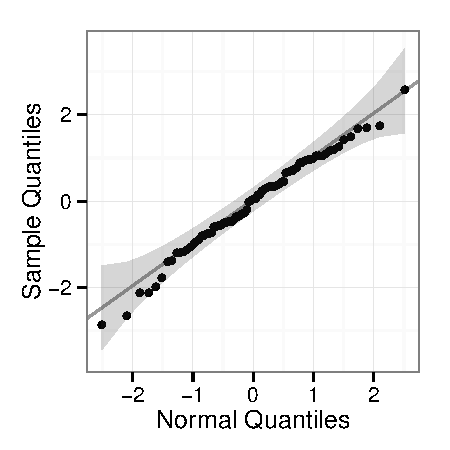
\includegraphics[width=\linewidth]{lcr-intercept-qq.pdf}
		\caption{Random intercepts}
	  \end{subfigure}	
	  \begin{subfigure}[b]{0.3\linewidth}
	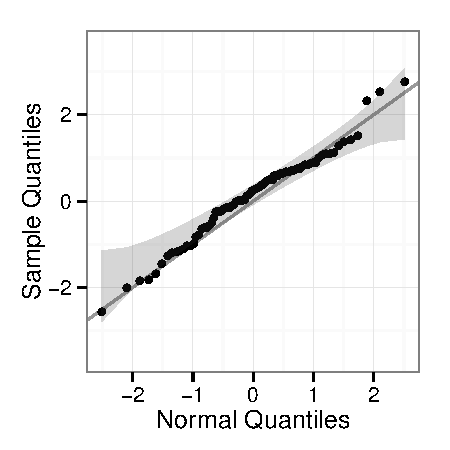
\includegraphics[width=\linewidth]{lcr-slope-qq.pdf}
		\caption{Random slopes}
	  \end{subfigure}	
%	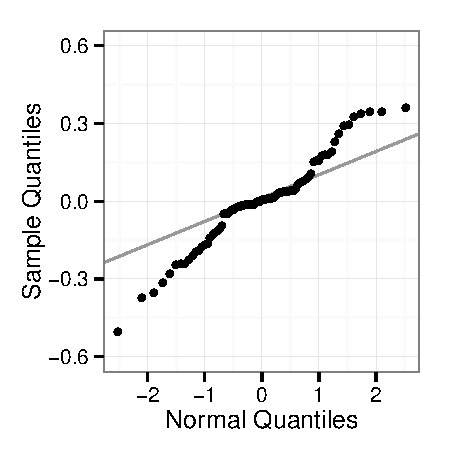
\includegraphics[width=0.32\textwidth]{raw-slope-qq.pdf}
	\caption{\label{fig:lcqq} Normal Q-Q plots of the minimally confounded random structures. The deviation from normality are much less pronounced than before -- in fact, it is questionable whether there is a significant amount of deviation; the results from the normal tests are not conclusive.}
\end{figure}

\begin{table}[ht]
\caption{\label{tab:edf2} Proportions of tests rejecting the null hypothesis of normality of the predicted error terms and random effects at the .05 significance level. 
}
\begin{center}
\begin{tabular}{l rrrr} \hline
 & \multicolumn{4}{c}{Test} \\  \cline{2-5}
 Residual & SW &  AD & CVM & KS \\ \hline
Error term			& 0.06 & 0.05 & 0.05 & 0.04 \\
Random intercept 	& \bf 0.04 & \bf 0.05 & \bf 0.05 & \bf 0.05 \\
Random slope 		& \bf 0.04 & \bf 0.04 & \bf 0.05 & \bf 0.05 \\
   \hline
\end{tabular}
\end{center}
\end{table}

\section{Exploring the Rotation Matrix}

The interpretation of minimally confounded residuals for purposes other than distributional assessment is complicated by the fact that they are linear combinations of residuals; however, the weights, $\bm{W}\trans$, are known, so interpretation is possible. Notice that the rows of $\bm{W}\trans$ give the weights specifying each linear combination and the columns give the weights assigned to each raw residual. Thus, the columns provide insight into the overall contribution of each raw residual and the rows of $\bm{W}\trans$ provide additional diagnostic information that, for example, can be used to investigate identified. In this section, each aspect will be investigated. To begin we explore the columns to better understand the rotation.

The average weights for each raw residual (column) show that residuals receiving larger weights are located in the center of the distribution of the raw residuals, while residuals receiving less weight are in the tails of the distribution. This is illustrated in Figure~\ref{fig:tailwts} for the predicted random effects using a linked histogram of average weights (right) and Q-Q plot of raw residuals (left).
%
\begin{figure}[htbp]
	\centering
	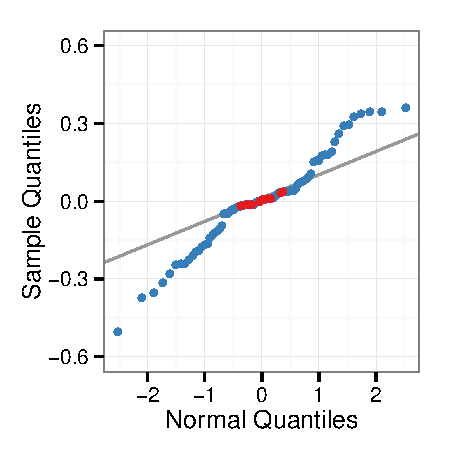
\includegraphics[width=0.4\linewidth]{qq-wts-tail.pdf}
	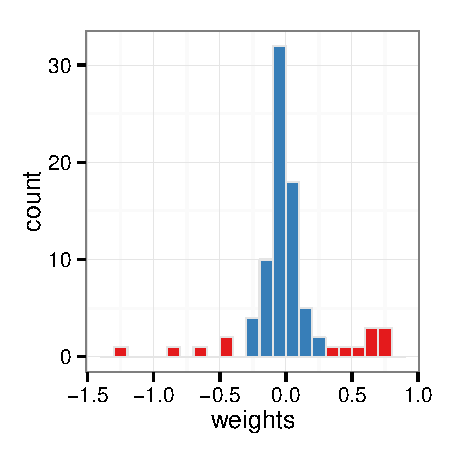
\includegraphics[width=0.4\linewidth]{hist-wts-tail.pdf}
	\caption{\label{fig:tailwts} Q-Q plot (left) and histogram (right) of the average weight for each raw residual given by $\bm{W}\trans$. The largest weights (red) correspond to residuals in the central region of the distribution of raw residuals.}
\end{figure}
%
To gain further insight, we must consider the entries of weight matrix.
%the two elements that comprise the rotation matrix: the relative precision factor of $\bm{B}$, $ \bm{\Lambda_r}^{-1/2} \bm{T_r}\trans$, and the orthogonal rotation matrix, $\bm{U}$.

\begin{figure*}[htb]
\centering
	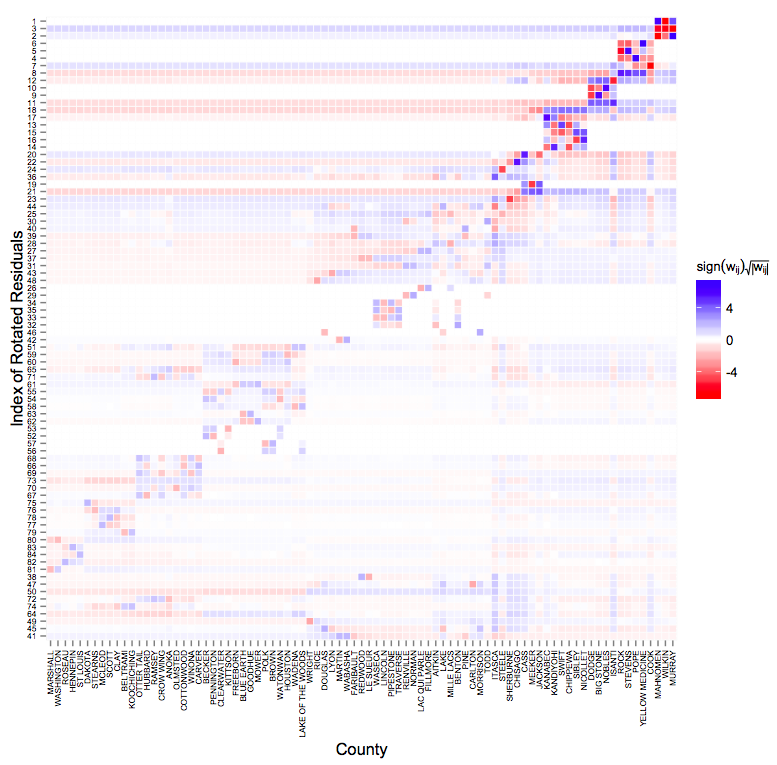
\includegraphics[width=0.9\textwidth]{tmslope-image.png}
	\caption{\label{fig:matimage} Heat map of $\bm{W}\trans$ for the predicted random slopes ordered by the variance of the predicted random effects. The entries were transformed to improve interpretability.
	}
	
\end{figure*}

Figure~\ref{fig:matimage} is a heat map of the  matrix of weights $\bm{W}$ for predicted random slopes  ordered by the variance of the predicted random slopes (with highest variance on the right).  Note that entries are scaled to their signed square root because of skewness in the weights. A block diagonal structure becomes apparent  in the heat map. This indicates  that terms with similar variances are treated similarly in the rotation to the least confounded direction. For example, Wilkin, Murray, and Mahnomen counties have the most variable predictions and are clustered together at the top right. Additionally, the horizontal lines that appear in the top portion of the heat map align with more confounded residuals, showing how information is combined to address this issue. Looking at the rows of the heat map will also aid in the interpretation of outlying points to determine whether a few observations are dominant or if many observations contribute equally.


%The relative precision factor of $\bm{B}$ performs the variance-covariance standardization of the residuals, and provides information about the relationships between residuals. Figure~\ref{fig:matimage} is a heat map of the relative precision factor for the variance of the predicted random slope that has been ordered by the variance of the predicted random slopes (with highest variance on the right). To aid interpretability, the entries were transformed into their signed square root. There is a clear block diagonal structure in this heat map that reveals counties with similar variances. For example, Wilkin, Murray, and Mahnomen counties have the most variable predictions and are clustered together at the top right. Additionally, the horizontal lines, which diminish from top right to bottom left, align with the amount of confounding in each predicted random slope. This matches expectations, since the confounding and pooling are interrelated, and estimates corresponding to highly confounded residuals will have a higher levels of pooling.

%For example, if an outlier is detected using the least confounded residuals, examination of the entries in the corresponding row of $\bm{M}\trans$ will reveal whether a few observations are dominant or if many contribute equally.



\section{Discussion}
We have shown that minimally confounded residuals are standardized, uncorrelated, homoscedastic residuals that address the concerns arising from the use of residuals for distributional assessment in the presence of pooling. The minimally confounded residuals can be used with Q-Q plots, which are familiar to analysts. While these residuals simplify the investigation of distributional assessment, they are linear combinations of residuals, and as such, are not directly applicable to the assessment of other aspects of the model, such as outlier detection; however, an investigation of the weights enables further investigation of unusual observations.
%
%however, investigation of the rotation matrix, $\bm{M}$, is itself of diagnostic interest.
%
%The rotation matrix, $\bm{M}$, is composed of the inverse square root matrix of the target residual, $ \bm{\Lambda_r}^{-1/2} \bm{T_r}\trans$,  and an orthogonal rotation matrix, $\bm{U}$. Both of these matrices are of diagnostic interest. Examination of the inverse square root matrix 
%
%\todo[inline]{I still need to figure out what to say about these matrices individually. I have been looking into them, and am still formulating what information they give us.}
%
It is important to note that goodness-of-fit tests are available for residuals at each level of the model \citep{Jiang:2001up}, but they do not lend themselves to graphical inspection, which is the focus of this paper, and the largely preferred method of distributional assessment. 

\section*{Appendix: Proof of Theorem I}

We present the proof of theorem~\ref{thm1}. To remain general we present our derivation in terms of the residual under investigation (the target residual), $\widehat{\bm{e}}$, which can refer to either $\widehat{\bm{\varepsilon}}$ or $\widehat{\bm{b}}$. 

We want to find a full rank matrix $\bm{W}$ that minimizes 
\begin{equation}\label{eq:app1}
\min_{W \in \mathbb{R}^{\ell-r \times \ell} } 
\displaystyle{\sum_i} \frac{\bm{v_i}\trans \bm{W} \var(\widehat{\bm{e}} | \bm{e}) \bm{W}\trans \bm{v_i}}
		{\bm{v_i}\trans \bm{W} \var(\widehat{\bm{e}}) \bm{W}\trans \bm{v_i}}
\end{equation}

\begin{proof}
 Let $\bm{A} = \var(\widehat{\bm{e}} | \bm{e})$, $\bm{B} = \var(\widehat{\bm{e}})$, $r = \text{rank}(\bm{B})$, and $\ell = $ the number of elements in $\widehat{\bm{e}}$. By definition $\bm{A}$ and $\bm{B}$ are symmetric and nonnegative definite. Write the spectral decomposition of $\bm{B}$ as
$\bm{B} = \bm{T_r \Lambda_r T_r}\trans$, where $\bm{ \Lambda_r}$ is a diagonal matrix of the nonzero eigenvalues and $\bm{T_r}$ is the matrix of associated eigenvectors.

Define $\bm{F} = \bm{T_r \Lambda_r}^{1/2}$, which is a full-rank decomposition of $\bm{B}$. The Moore-Penrose inverse of $\bm{F}$ is given by
\[
\bm{F}\ginv = (\bm{F}\trans\bm{F})\inv \bm{F}\trans = \bm{\Lambda_r}^{-1/2} \bm{T_r}\trans
\]
Now, notice that
\[
\bm{F}\ginv \bm{B} (\bm{F}\ginv)\trans = \bm{\Lambda_r}^{-1/2} \bm{T_r}\trans ( \bm{T_r \Lambda_r T_r}\trans ) \bm{T_r \Lambda_r}^{-1/2} =  \bm{I}
\]

If we consider $\bm{w}_i = (\bm{F}\ginv)\trans \bm{u}_i$, then we find that 
\begin{equation}\label{eq:app2}
\frac{\bm{w_i}\trans A \bm{w_i}}{\bm{w_i}\trans B \bm{w_i}} = 
\frac{\bm{u_i}\trans (\bm{F}\ginv) \bm{A} (\bm{F}\ginv)\trans \bm{u_i}}{\bm{u_i}\trans(\bm{F}\ginv) \bm{B} (\bm{F}\ginv)\trans \bm{w_i}} = 
\frac{\bm{u_i} \bm{A}^* \bm{u_i}}{\bm{u_i}\trans \bm{u_i}}
\end{equation}

which is of the form of an eigenvalue problem, which is minimized at the eigenvector corresponding to the smallest eigenvalue of  $\bm{A}^*$. Additionally, the value of \eqref{eq:app2} lies between the minimum and maximum eigenvalue of $\bm{A}^*$.

The requirement that $\bm{W}$ be of full rank results in $\bm{W} = \bm{T_r \Lambda_r}^{-1/2} \bm{U}$, where $\bm{U}$ are the eigenvectors of $\bm{A}^*$.
\end{proof}

More general proofs can be found in \cite{McDonald:1979ca} and \cite{deLeeuw:1982to}.

Next we show that the resulting residuals are standardized, uncorrelated, and homoscedastic.

\begin{proof} Carrying through the notation from above we see that
\begin{align*}
\var(\bm{W}\trans \widehat{\bm{e}}) &= \var(\bm{U}\trans \bm{\Lambda_r}^{-1/2} \bm{T_r}\trans \widehat{\bm{e}})\\
&= (\bm{U}\trans \bm{\Lambda_r}^{-1/2} \bm{T_r}\trans) \var(\widehat{\bm{e}}) (\bm{T_r \Lambda_r}^{-1/2} \bm{U})\\
&= (\bm{U}\trans \bm{\Lambda_r}^{-1/2} \bm{T_r}\trans) \bm{B} (\bm{T_r \Lambda_r}^{-1/2} \bm{U})\\
&= \bm{I}
\end{align*}

\end{proof}


%----------------------------------------------------------------------------------
%----------------------------------------------------------------------------------
\bibliographystyle{apa}
\bibliography{lcresid_bib}
%----------------------------------------------------------------------------------
%----------------------------------------------------------------------------------

\section*{Simulation results}

%----------------------------------------------------------------------------------
%----------------------------------------------------------------------------------

%------------------------------------------------
% Naive tests
%------------------------------------------------

%%% Random intercept
\begin{table}[ht]
\caption{Naive tests for normality of the random intercept using three rotations.}
\begin{scriptsize}
\begin{center}
\begin{tabular}{ll p{.1cm} c p{.1cm} rrr p{.1cm} rrr p{.1cm} rrr}
  \hline
  \multicolumn{2}{c}{Distributions}& & Nominal & &  \multicolumn{3}{c}{Rotation 1} & & \multicolumn{3}{c}{Rotation 2} & & \multicolumn{3}{c}{Rotation 3}\\ \cline{1-2} \cline{6-8} \cline{10-12} \cline{14-16}
  Random effects & Errors & & $\alpha$ & & AD & CVM & KS & & AD & CVM & KS & & AD & CVM & KS \\ 
   \hline
& && && \multicolumn{9}{c}{$\sigma_{\varepsilon}^2 = 4$, \ \ $\sigma_{b_0}^2 = \sigma_{b_1}^2 = 1$} \\ \cline{6-16}
\rowcolor{gray!20}Normal       & Normal       && 0.05 &&   0.05 & 0.05 & 0.06 && 0.08 & 0.07 & 0.07 && 0.08 & 0.07 & 0.07 \\ 
\rowcolor{gray!20}             &              && 0.10 &&   0.09 & 0.10 & 0.11 && 0.14 & 0.13 & 0.12 && 0.14 & 0.13 & 0.12 \\ 
\rowcolor{gray!20}             & Heavy tailed && 0.05 &&   0.08 & 0.07 & 0.08 && 0.12 & 0.11 & 0.10 && 0.12 & 0.11 & 0.10 \\ 
\rowcolor{gray!20}             &              && 0.10 &&   0.14 & 0.13 & 0.13 && 0.19 & 0.18 & 0.16 && 0.19 & 0.18 & 0.16 \\ 
\rowcolor{gray!20}             & Skewed       && 0.05 &&   0.05 & 0.05 & 0.04 && 0.10 & 0.09 & 0.09 && 0.10 & 0.09 & 0.09 \\ 
\rowcolor{gray!20}             &              && 0.10 &&   0.10 & 0.10 & 0.10 && 0.17 & 0.16 & 0.14 && 0.17 & 0.16 & 0.14 \\ 
             &&&&&&&&&&&&&&&\\
Heavy tailed & Normal       && 0.05 &&   0.15 & 0.14 & 0.11 && 0.23 & 0.20 & 0.16 && 0.23 & 0.20 & 0.16 \\ 
             &              && 0.10 &&   0.21 & 0.20 & 0.20 && 0.31 & 0.28 & 0.25 && 0.31 & 0.28 & 0.25 \\ 
             & Heavy tailed && 0.05 &&   0.20 & 0.18 & 0.14 && 0.33 & 0.29 & 0.23 && 0.33 & 0.29 & 0.23 \\ 
             &              && 0.10 &&   0.29 & 0.26 & 0.23 && 0.43 & 0.40 & 0.34 && 0.43 & 0.40 & 0.34 \\ 
             & Skewed       && 0.05 &&   0.19 & 0.17 & 0.14 && 0.29 & 0.26 & 0.20 && 0.29 & 0.26 & 0.20 \\ 
             &              && 0.10 &&   0.26 & 0.24 & 0.22 && 0.40 & 0.36 & 0.30 && 0.40 & 0.36 & 0.30 \\ 
             &&&&&&&&&&&&&&&\\
Skewed       & Normal       && 0.05 &&   0.10 & 0.09 & 0.07 && 0.17 & 0.14 & 0.10 && 0.17 & 0.14 & 0.10 \\ 
             &              && 0.10 &&   0.15 & 0.15 & 0.14 && 0.24 & 0.21 & 0.19 && 0.24 & 0.21 & 0.19 \\ 
             & Heavy tailed && 0.05 &&   0.17 & 0.15 & 0.13 && 0.29 & 0.26 & 0.20 && 0.29 & 0.26 & 0.20 \\ 
             &              && 0.10 &&   0.26 & 0.24 & 0.22 && 0.38 & 0.35 & 0.29 && 0.38 & 0.35 & 0.29 \\ 
             & Skewed       && 0.05 &&   0.12 & 0.10 & 0.08 && 0.20 & 0.17 & 0.13 && 0.20 & 0.17 & 0.13 \\ 
             &              && 0.10 &&   0.19 & 0.17 & 0.15 && 0.29 & 0.26 & 0.22 && 0.29 & 0.26 & 0.22 \\ 


&&&&&&&&&&&&&&&\\
& && && \multicolumn{9}{c}{$\sigma_{\varepsilon}^2 = 1$, \ \ $\sigma_{b_0}^2 = \sigma_{b_1}^2 = 1$} \\ \cline{6-16}
\rowcolor{gray!20}Normal       & Normal       && 0.05 &&   0.04 & 0.05 & 0.05 && 0.05 & 0.05 & 0.04 && 0.05 & 0.05 & 0.04 \\ 
\rowcolor{gray!20}             &              && 0.10 &&   0.09 & 0.09 & 0.09 && 0.10 & 0.10 & 0.10 && 0.10 & 0.10 & 0.10 \\ 
\rowcolor{gray!20}             & Heavy tailed && 0.05 &&   0.07 & 0.07 & 0.07 && 0.07 & 0.08 & 0.07 && 0.07 & 0.08 & 0.07 \\ 
\rowcolor{gray!20}             &              && 0.10 &&   0.12 & 0.11 & 0.11 && 0.12 & 0.11 & 0.11 && 0.12 & 0.11 & 0.11 \\ 
\rowcolor{gray!20}             & Skewed       && 0.05 &&   0.05 & 0.05 & 0.05 && 0.06 & 0.06 & 0.06 && 0.06 & 0.06 & 0.06 \\ 
\rowcolor{gray!20}             &              && 0.10 &&   0.11 & 0.11 & 0.11 && 0.12 & 0.12 & 0.11 && 0.12 & 0.12 & 0.11 \\ 
             &&&&&&&&&&&&&&&\\
Heavy tailed & Normal       && 0.05 &&   0.26 & 0.23 & 0.20 && 0.27 & 0.24 & 0.20 && 0.27 & 0.24 & 0.20 \\ 
             &              && 0.10 &&   0.33 & 0.30 & 0.28 && 0.36 & 0.33 & 0.29 && 0.36 & 0.33 & 0.29 \\ 
             & Heavy tailed && 0.05 &&   0.29 & 0.26 & 0.20 && 0.32 & 0.28 & 0.22 && 0.32 & 0.28 & 0.22 \\ 
             &              && 0.10 &&   0.37 & 0.34 & 0.30 && 0.40 & 0.38 & 0.32 && 0.40 & 0.38 & 0.32 \\ 
             & Skewed       && 0.05 &&   0.28 & 0.25 & 0.22 && 0.30 & 0.28 & 0.23 && 0.30 & 0.28 & 0.23 \\ 
             &              && 0.10 &&   0.37 & 0.33 & 0.30 && 0.39 & 0.36 & 0.32 && 0.39 & 0.36 & 0.32 \\ 
             &&&&&&&&&&&&&&&\\
Skewed       & Normal       && 0.05 &&   0.20 & 0.17 & 0.12 && 0.22 & 0.19 & 0.14 && 0.22 & 0.19 & 0.14 \\ 
             &              && 0.10 &&   0.30 & 0.27 & 0.22 && 0.31 & 0.28 & 0.23 && 0.31 & 0.28 & 0.23 \\ 
             & Heavy tailed && 0.05 &&   0.26 & 0.23 & 0.17 && 0.29 & 0.25 & 0.18 && 0.29 & 0.25 & 0.18 \\ 
             &              && 0.10 &&   0.37 & 0.32 & 0.27 && 0.38 & 0.34 & 0.28 && 0.38 & 0.34 & 0.28 \\ 
             & Skewed       && 0.05 &&   0.21 & 0.18 & 0.12 && 0.24 & 0.20 & 0.14 && 0.24 & 0.20 & 0.14 \\ 
             &              && 0.10 &&   0.28 & 0.25 & 0.21 && 0.31 & 0.28 & 0.21 && 0.31 & 0.28 & 0.21 \\ 


&&&&&&&&&&&&&&&\\
& && && \multicolumn{9}{c}{$\sigma_{\varepsilon}^2 = 1$, \ \ $\sigma_{b_0}^2 = \sigma_{b_1}^2 = 4$} \\ \cline{6-16}
\rowcolor{gray!20}Normal       & Normal       && 0.05 &&   0.05 & 0.05 & 0.07 && 0.05 & 0.04 & 0.07 && 0.05 & 0.04 & 0.07 \\ 
\rowcolor{gray!20}             &              && 0.10 &&   0.10 & 0.10 & 0.10 && 0.10 & 0.11 & 0.11 && 0.10 & 0.11 & 0.11 \\ 
\rowcolor{gray!20}             & Heavy tailed && 0.05 &&   0.06 & 0.06 & 0.06 && 0.06 & 0.06 & 0.06 && 0.06 & 0.06 & 0.06 \\ 
\rowcolor{gray!20}             &              && 0.10 &&   0.12 & 0.12 & 0.11 && 0.12 & 0.12 & 0.11 && 0.12 & 0.12 & 0.11 \\ 
\rowcolor{gray!20}             & Skewed       && 0.05 &&   0.06 & 0.06 & 0.06 && 0.06 & 0.06 & 0.06 && 0.06 & 0.06 & 0.06 \\ 
\rowcolor{gray!20}             &              && 0.10 &&   0.11 & 0.11 & 0.12 && 0.11 & 0.11 & 0.12 && 0.11 & 0.11 & 0.12 \\ 
             &&&&&&&&&&&&&&&\\
Heavy tailed & Normal       && 0.05 &&   0.38 & 0.35 & 0.30 && 0.38 & 0.35 & 0.30 && 0.38 & 0.35 & 0.30 \\ 
             &              && 0.10 &&   0.46 & 0.42 & 0.38 && 0.47 & 0.43 & 0.39 && 0.47 & 0.43 & 0.39 \\ 
             & Heavy tailed && 0.05 &&   0.38 & 0.34 & 0.28 && 0.38 & 0.35 & 0.27 && 0.38 & 0.35 & 0.27 \\ 
             &              && 0.10 &&   0.47 & 0.43 & 0.38 && 0.48 & 0.45 & 0.39 && 0.48 & 0.45 & 0.39 \\ 
             & Skewed       && 0.05 &&   0.35 & 0.32 & 0.25 && 0.35 & 0.32 & 0.26 && 0.35 & 0.32 & 0.26 \\ 
             &              && 0.10 &&   0.44 & 0.41 & 0.35 && 0.45 & 0.41 & 0.36 && 0.45 & 0.41 & 0.36 \\ 
             &&&&&&&&&&&&&&&\\
Skewed       & Normal       && 0.05 &&   0.30 & 0.27 & 0.20 && 0.30 & 0.27 & 0.20 && 0.30 & 0.27 & 0.20 \\ 
             &              && 0.10 &&   0.39 & 0.36 & 0.31 && 0.39 & 0.36 & 0.30 && 0.39 & 0.36 & 0.30 \\ 
             & Heavy tailed && 0.05 &&   0.32 & 0.28 & 0.22 && 0.32 & 0.29 & 0.21 && 0.32 & 0.29 & 0.21 \\ 
             &              && 0.10 &&   0.41 & 0.37 & 0.32 && 0.42 & 0.37 & 0.33 && 0.42 & 0.37 & 0.33 \\ 
             & Skewed       && 0.05 &&   0.27 & 0.23 & 0.17 && 0.27 & 0.23 & 0.17 && 0.27 & 0.23 & 0.17 \\ 
             &              && 0.10 &&   0.37 & 0.33 & 0.27 && 0.37 & 0.33 & 0.26 && 0.37 & 0.33 & 0.26 \\ 

   \hline
\end{tabular}
\end{center}
\end{scriptsize}
\end{table}


\begin{table}[ht]
\caption{Naive tests for normality of the random intercept using three varimax rotations.}
\begin{scriptsize}
\begin{center}
\begin{tabular}{ll p{.1cm} c p{.1cm} rrr p{.1cm} rrr p{.1cm} rrr}
  \hline
  \multicolumn{2}{c}{Distributions}& & Nominal & &  \multicolumn{3}{c}{Rotation 1} & & \multicolumn{3}{c}{Rotation 2} & & \multicolumn{3}{c}{Rotation 3}\\ \cline{1-2} \cline{6-8} \cline{10-12} \cline{14-16}
  Random effects & Errors & & $\alpha$ & & AD & CVM & KS & & AD & CVM & KS & & AD & CVM & KS \\ 
   \hline
& && && \multicolumn{9}{c}{$\sigma_{\varepsilon}^2 = 4$, \ \ $\sigma_{b_0}^2 = \sigma_{b_1}^2 = 1$} \\ \cline{6-16}
\rowcolor{gray!20}Normal       & Normal       && 0.05 &&   0.07 & 0.06 & 0.06 && 0.09 & 0.09 & 0.07 && 0.09 & 0.09 & 0.07 \\ 
\rowcolor{gray!20}             &              && 0.10 &&   0.11 & 0.11 & 0.10 && 0.14 & 0.14 & 0.13 && 0.14 & 0.14 & 0.13 \\ 
\rowcolor{gray!20}             & Heavy tailed && 0.05 &&   0.13 & 0.12 & 0.09 && 0.16 & 0.15 & 0.13 && 0.16 & 0.15 & 0.13 \\ 
\rowcolor{gray!20}             &              && 0.10 &&   0.18 & 0.18 & 0.17 && 0.26 & 0.23 & 0.22 && 0.26 & 0.23 & 0.22 \\ 
\rowcolor{gray!20}             & Skewed       && 0.05 &&   0.07 & 0.06 & 0.07 && 0.10 & 0.09 & 0.07 && 0.10 & 0.09 & 0.07 \\ 
\rowcolor{gray!20}             &              && 0.10 &&   0.13 & 0.13 & 0.12 && 0.18 & 0.15 & 0.14 && 0.18 & 0.15 & 0.14 \\ 
             &&&&&&&&&&&&&&&\\
Heavy tailed & Normal       && 0.05 &&   0.28 & 0.24 & 0.20 && 0.38 & 0.33 & 0.25 && 0.38 & 0.33 & 0.25 \\ 
             &              && 0.10 &&   0.36 & 0.33 & 0.28 && 0.47 & 0.42 & 0.36 && 0.47 & 0.42 & 0.36 \\ 
             & Heavy tailed && 0.05 &&   0.45 & 0.41 & 0.31 && 0.58 & 0.53 & 0.42 && 0.58 & 0.53 & 0.42 \\ 
             &              && 0.10 &&   0.55 & 0.48 & 0.43 && 0.68 & 0.64 & 0.53 && 0.68 & 0.64 & 0.53 \\ 
             & Skewed       && 0.05 &&   0.33 & 0.30 & 0.22 && 0.48 & 0.41 & 0.33 && 0.48 & 0.41 & 0.33 \\ 
             &              && 0.10 &&   0.44 & 0.37 & 0.32 && 0.58 & 0.53 & 0.44 && 0.58 & 0.53 & 0.44 \\
             &&&&&&&&&&&&&&&\\ 
Skewed       & Normal       && 0.05 &&   0.20 & 0.17 & 0.13 && 0.29 & 0.24 & 0.18 && 0.29 & 0.24 & 0.18 \\ 
             &              && 0.10 &&   0.29 & 0.24 & 0.20 && 0.39 & 0.34 & 0.29 && 0.39 & 0.34 & 0.29 \\ 
             & Heavy tailed && 0.05 &&   0.40 & 0.32 & 0.23 && 0.48 & 0.41 & 0.31 && 0.48 & 0.41 & 0.31 \\ 
             &              && 0.10 &&   0.51 & 0.44 & 0.35 && 0.59 & 0.52 & 0.42 && 0.59 & 0.52 & 0.42 \\ 
             & Skewed       && 0.05 &&   0.27 & 0.18 & 0.14 && 0.32 & 0.23 & 0.18 && 0.32 & 0.23 & 0.18 \\ 
             &              && 0.10 &&   0.36 & 0.29 & 0.23 && 0.44 & 0.33 & 0.27 && 0.44 & 0.33 & 0.27 \\ 

&&&&&&&&&&&&&&&\\
& && && \multicolumn{9}{c}{$\sigma_{\varepsilon}^2 = 1$, \ \ $\sigma_{b_0}^2 = \sigma_{b_1}^2 = 1$} \\ \cline{6-16}
\rowcolor{gray!20}Normal       & Normal       && 0.05 &&   0.05 & 0.05 & 0.06 && 0.05 & 0.05 & 0.06 && 0.05 & 0.05 & 0.06 \\ 
\rowcolor{gray!20}             &              && 0.10 &&   0.09 & 0.09 & 0.10 && 0.10 & 0.09 & 0.10 && 0.10 & 0.09 & 0.10 \\ 
\rowcolor{gray!20}             & Heavy tailed && 0.05 &&   0.07 & 0.07 & 0.06 && 0.08 & 0.07 & 0.06 && 0.08 & 0.07 & 0.06 \\ 
\rowcolor{gray!20}             &              && 0.10 &&   0.12 & 0.12 & 0.11 && 0.14 & 0.13 & 0.12 && 0.14 & 0.13 & 0.12 \\ 
\rowcolor{gray!20}             & Skewed       && 0.05 &&   0.07 & 0.06 & 0.05 && 0.07 & 0.06 & 0.07 && 0.07 & 0.06 & 0.07 \\ 
\rowcolor{gray!20}             &              && 0.10 &&   0.13 & 0.13 & 0.10 && 0.13 & 0.13 & 0.12 && 0.13 & 0.13 & 0.12 \\ 
             &&&&&&&&&&&&&&&\\
Heavy tailed & Normal       && 0.05 &&   0.49 & 0.45 & 0.36 && 0.52 & 0.45 & 0.40 && 0.52 & 0.45 & 0.40 \\ 
             &              && 0.10 &&   0.56 & 0.51 & 0.46 && 0.59 & 0.56 & 0.49 && 0.59 & 0.56 & 0.49 \\ 
             & Heavy tailed && 0.05 &&   0.58 & 0.54 & 0.44 && 0.60 & 0.55 & 0.45 && 0.60 & 0.55 & 0.45 \\ 
             &              && 0.10 &&   0.66 & 0.63 & 0.55 && 0.69 & 0.65 & 0.55 && 0.69 & 0.65 & 0.55 \\ 
             & Skewed       && 0.05 &&   0.54 & 0.48 & 0.41 && 0.56 & 0.50 & 0.41 && 0.56 & 0.50 & 0.41 \\ 
             &              && 0.10 &&   0.64 & 0.58 & 0.52 && 0.65 & 0.60 & 0.53 && 0.65 & 0.60 & 0.53 \\ 
             &&&&&&&&&&&&&&&\\
Skewed       & Normal       && 0.05 &&   0.43 & 0.34 & 0.24 && 0.46 & 0.35 & 0.24 && 0.46 & 0.35 & 0.24 \\ 
             &              && 0.10 &&   0.55 & 0.46 & 0.35 && 0.56 & 0.46 & 0.38 && 0.56 & 0.46 & 0.38 \\ 
             & Heavy tailed && 0.05 &&   0.50 & 0.41 & 0.33 && 0.51 & 0.41 & 0.33 && 0.51 & 0.41 & 0.33 \\ 
             &              && 0.10 &&   0.60 & 0.50 & 0.43 && 0.60 & 0.50 & 0.44 && 0.60 & 0.50 & 0.44 \\ 
             & Skewed       && 0.05 &&   0.43 & 0.31 & 0.23 && 0.46 & 0.33 & 0.24 && 0.46 & 0.33 & 0.24 \\ 
             &              && 0.10 &&   0.55 & 0.41 & 0.33 && 0.57 & 0.43 & 0.35 && 0.57 & 0.43 & 0.35 \\ 


&&&&&&&&&&&&&&&\\
& && && \multicolumn{9}{c}{$\sigma_{\varepsilon}^2 = 1$, \ \ $\sigma_{b_0}^2 = \sigma_{b_1}^2 = 4$} \\ \cline{6-16}
\rowcolor{gray!20}Normal       & Normal       && 0.05 &&   0.05 & 0.05 & 0.05 && 0.05 & 0.05 & 0.05 && 0.05 & 0.05 & 0.05 \\ 
\rowcolor{gray!20}             &              && 0.10 &&   0.09 & 0.09 & 0.10 && 0.09 & 0.09 & 0.10 && 0.09 & 0.09 & 0.10 \\ 
\rowcolor{gray!20}             & Heavy tailed && 0.05 &&   0.06 & 0.06 & 0.06 && 0.05 & 0.05 & 0.05 && 0.05 & 0.05 & 0.05 \\ 
\rowcolor{gray!20}             &              && 0.10 &&   0.10 & 0.10 & 0.11 && 0.09 & 0.10 & 0.11 && 0.09 & 0.10 & 0.11 \\ 
\rowcolor{gray!20}             & Skewed       && 0.05 &&   0.06 & 0.06 & 0.05 && 0.05 & 0.06 & 0.05 && 0.05 & 0.06 & 0.05 \\ 
\rowcolor{gray!20}             &              && 0.10 &&   0.11 & 0.10 & 0.11 && 0.11 & 0.10 & 0.11 && 0.11 & 0.10 & 0.11 \\ 
             &&&&&&&&&&&&&&&\\
Heavy tailed & Normal       && 0.05 &&   0.62 & 0.59 & 0.48 && 0.64 & 0.60 & 0.50 && 0.64 & 0.60 & 0.50 \\ 
             &              && 0.10 &&   0.71 & 0.67 & 0.58 && 0.72 & 0.68 & 0.60 && 0.72 & 0.68 & 0.60 \\ 
             & Heavy tailed && 0.05 &&   0.67 & 0.63 & 0.53 && 0.69 & 0.65 & 0.56 && 0.69 & 0.65 & 0.56 \\ 
             &              && 0.10 &&   0.74 & 0.71 & 0.63 && 0.75 & 0.73 & 0.65 && 0.75 & 0.73 & 0.65 \\ 
             & Skewed       && 0.05 &&   0.67 & 0.61 & 0.51 && 0.68 & 0.63 & 0.52 && 0.68 & 0.63 & 0.52 \\ 
             &              && 0.10 &&   0.74 & 0.69 & 0.60 && 0.75 & 0.71 & 0.61 && 0.75 & 0.71 & 0.61 \\
             &&&&&&&&&&&&&&&\\ 
Skewed       & Normal       && 0.05 &&   0.60 & 0.46 & 0.37 && 0.63 & 0.48 & 0.37 && 0.63 & 0.48 & 0.37 \\ 
             &              && 0.10 &&   0.70 & 0.59 & 0.50 && 0.73 & 0.60 & 0.50 && 0.73 & 0.60 & 0.50 \\ 
             & Heavy tailed && 0.05 &&   0.64 & 0.51 & 0.41 && 0.64 & 0.52 & 0.43 && 0.64 & 0.52 & 0.43 \\ 
             &              && 0.10 &&   0.76 & 0.63 & 0.54 && 0.75 & 0.62 & 0.54 && 0.75 & 0.62 & 0.54 \\ 
             & Skewed       && 0.05 &&   0.62 & 0.46 & 0.36 && 0.62 & 0.47 & 0.35 && 0.62 & 0.47 & 0.35 \\ 
             &              && 0.10 &&   0.73 & 0.59 & 0.49 && 0.73 & 0.59 & 0.48 && 0.73 & 0.59 & 0.48 \\ 


   \hline
\end{tabular}
\end{center}
\end{scriptsize}
\end{table}



%%% Random slope
\begin{table}[ht]
\caption{Naive tests for normality of the random slope using three rotations.}
\begin{scriptsize}
\begin{center}
\begin{tabular}{ll p{.1cm} c p{.1cm} rrr p{.1cm} rrr p{.1cm} rrr}
  \hline
  \multicolumn{2}{c}{Distributions}& & Nominal & &  \multicolumn{3}{c}{Rotation 1} & & \multicolumn{3}{c}{Rotation 2} & & \multicolumn{3}{c}{Rotation 3}\\ \cline{1-2} \cline{6-8} \cline{10-12} \cline{14-16}
  Random effects & Errors & & $\alpha$ & & AD & CVM & KS & & AD & CVM & KS & & AD & CVM & KS \\ 
   \hline
& && && \multicolumn{9}{c}{$\sigma_{\varepsilon}^2 = 4$, \ \ $\sigma_{b_0}^2 = \sigma_{b_1}^2 = 1$} \\ \cline{6-16}
\rowcolor{gray!20}Normal       & Normal       && 0.05 &&   0.04 & 0.04 & 0.04 && 0.12 & 0.10 & 0.08 && 0.12 & 0.10 & 0.08 \\ 
\rowcolor{gray!20}             &              && 0.10 &&   0.09 & 0.09 & 0.10 && 0.19 & 0.17 & 0.14 && 0.19 & 0.17 & 0.14 \\ 
\rowcolor{gray!20}             & Heavy tailed && 0.05 &&   0.14 & 0.14 & 0.12 && 0.25 & 0.23 & 0.18 && 0.25 & 0.23 & 0.18 \\ 
\rowcolor{gray!20}             &              && 0.10 &&   0.21 & 0.19 & 0.19 && 0.35 & 0.31 & 0.26 && 0.35 & 0.31 & 0.26 \\ 
\rowcolor{gray!20}             & Skewed       && 0.05 &&   0.10 & 0.10 & 0.08 && 0.19 & 0.18 & 0.13 && 0.19 & 0.18 & 0.13 \\ 
\rowcolor{gray!20}             &              && 0.10 &&   0.16 & 0.16 & 0.15 && 0.29 & 0.29 & 0.23 && 0.29 & 0.29 & 0.23 \\ 
             &&&&&&&&&&&&&&&\\
Heavy tailed & Normal       && 0.05 &&   0.07 & 0.07 & 0.05 && 0.15 & 0.13 & 0.10 && 0.15 & 0.13 & 0.10 \\ 
             &              && 0.10 &&   0.13 & 0.12 & 0.12 && 0.24 & 0.20 & 0.17 && 0.24 & 0.20 & 0.17 \\ 
             & Heavy tailed && 0.05 &&   0.21 & 0.20 & 0.17 && 0.36 & 0.33 & 0.24 && 0.36 & 0.33 & 0.24 \\ 
             &              && 0.10 &&   0.28 & 0.26 & 0.23 && 0.45 & 0.41 & 0.34 && 0.45 & 0.41 & 0.34 \\ 
             & Skewed       && 0.05 &&   0.14 & 0.13 & 0.10 && 0.25 & 0.21 & 0.17 && 0.25 & 0.21 & 0.17 \\ 
             &              && 0.10 &&   0.21 & 0.19 & 0.17 && 0.34 & 0.32 & 0.24 && 0.34 & 0.32 & 0.24 \\
             &&&&&&&&&&&&&&&\\ 
Skewed       & Normal       && 0.05 &&   0.07 & 0.06 & 0.06 && 0.15 & 0.13 & 0.11 && 0.15 & 0.13 & 0.11 \\ 
             &              && 0.10 &&   0.12 & 0.12 & 0.12 && 0.23 & 0.22 & 0.17 && 0.23 & 0.22 & 0.17 \\ 
             & Heavy tailed && 0.05 &&   0.15 & 0.13 & 0.12 && 0.29 & 0.26 & 0.20 && 0.29 & 0.26 & 0.20 \\ 
             &              && 0.10 &&   0.23 & 0.20 & 0.19 && 0.41 & 0.37 & 0.30 && 0.41 & 0.37 & 0.30 \\ 
             & Skewed       && 0.05 &&   0.10 & 0.08 & 0.07 && 0.19 & 0.16 & 0.12 && 0.19 & 0.16 & 0.12 \\ 
             &              && 0.10 &&   0.16 & 0.15 & 0.14 && 0.29 & 0.25 & 0.21 && 0.29 & 0.25 & 0.21 \\ 

&&&&&&&&&&&&&&&\\
& && && \multicolumn{9}{c}{$\sigma_{\varepsilon}^2 = 1$, \ \ $\sigma_{b_0}^2 = \sigma_{b_1}^2 = 1$} \\ \cline{6-16}
\rowcolor{gray!20}Normal       & Normal       && 0.05 &&   0.06 & 0.06 & 0.05 && 0.07 & 0.08 & 0.06 && 0.07 & 0.08 & 0.06 \\ 
\rowcolor{gray!20}             &              && 0.10 &&   0.12 & 0.12 & 0.10 && 0.14 & 0.14 & 0.13 && 0.14 & 0.14 & 0.13 \\ 
\rowcolor{gray!20}             & Heavy tailed && 0.05 &&   0.08 & 0.07 & 0.07 && 0.10 & 0.09 & 0.07 && 0.10 & 0.09 & 0.07 \\ 
\rowcolor{gray!20}             &              && 0.10 &&   0.14 & 0.13 & 0.11 && 0.16 & 0.15 & 0.12 && 0.16 & 0.15 & 0.12 \\ 
\rowcolor{gray!20}             & Skewed       && 0.05 &&   0.07 & 0.06 & 0.05 && 0.08 & 0.07 & 0.06 && 0.08 & 0.07 & 0.06 \\ 
\rowcolor{gray!20}             &              && 0.10 &&   0.12 & 0.12 & 0.10 && 0.15 & 0.14 & 0.10 && 0.15 & 0.14 & 0.10 \\ 
             &&&&&&&&&&&&&&&\\
Heavy tailed & Normal       && 0.05 &&   0.15 & 0.14 & 0.12 && 0.17 & 0.15 & 0.14 && 0.17 & 0.15 & 0.14 \\ 
             &              && 0.10 &&   0.22 & 0.20 & 0.20 && 0.25 & 0.23 & 0.21 && 0.25 & 0.23 & 0.21 \\ 
             & Heavy tailed && 0.05 &&   0.22 & 0.21 & 0.17 && 0.28 & 0.26 & 0.19 && 0.28 & 0.26 & 0.19 \\ 
             &              && 0.10 &&   0.31 & 0.28 & 0.24 && 0.35 & 0.32 & 0.29 && 0.35 & 0.32 & 0.29 \\ 
             & Skewed       && 0.05 &&   0.16 & 0.15 & 0.11 && 0.21 & 0.19 & 0.15 && 0.21 & 0.19 & 0.15 \\ 
             &              && 0.10 &&   0.25 & 0.23 & 0.20 && 0.29 & 0.26 & 0.23 && 0.29 & 0.26 & 0.23 \\ 
             &&&&&&&&&&&&&&&\\
Skewed       & Normal       && 0.05 &&   0.10 & 0.09 & 0.08 && 0.14 & 0.11 & 0.10 && 0.14 & 0.11 & 0.10 \\ 
             &              && 0.10 &&   0.17 & 0.16 & 0.15 && 0.22 & 0.20 & 0.17 && 0.22 & 0.20 & 0.17 \\ 
             & Heavy tailed && 0.05 &&   0.16 & 0.14 & 0.11 && 0.20 & 0.19 & 0.13 && 0.20 & 0.19 & 0.13 \\ 
             &              && 0.10 &&   0.24 & 0.21 & 0.17 && 0.29 & 0.25 & 0.21 && 0.29 & 0.25 & 0.21 \\ 
             & Skewed       && 0.05 &&   0.13 & 0.11 & 0.09 && 0.15 & 0.13 & 0.10 && 0.15 & 0.13 & 0.10 \\ 
             &              && 0.10 &&   0.19 & 0.18 & 0.14 && 0.23 & 0.21 & 0.17 && 0.23 & 0.21 & 0.17 \\ 


&&&&&&&&&&&&&&&\\
& && && \multicolumn{9}{c}{$\sigma_{\varepsilon}^2 = 1$, \ \ $\sigma_{b_0}^2 = \sigma_{b_1}^2 = 4$} \\ \cline{6-16}
\rowcolor{gray!20}Normal       & Normal       && 0.05 &&   0.05 & 0.05 & 0.04 && 0.05 & 0.05 & 0.04 && 0.05 & 0.05 & 0.04 \\ 
\rowcolor{gray!20}             &              && 0.10 &&   0.10 & 0.10 & 0.10 && 0.11 & 0.11 & 0.10 && 0.11 & 0.11 & 0.10 \\ 
\rowcolor{gray!20}             & Heavy tailed && 0.05 &&   0.07 & 0.07 & 0.07 && 0.07 & 0.07 & 0.07 && 0.07 & 0.07 & 0.07 \\ 
\rowcolor{gray!20}             &              && 0.10 &&   0.13 & 0.11 & 0.12 && 0.12 & 0.12 & 0.12 && 0.12 & 0.12 & 0.12 \\ 
\rowcolor{gray!20}             & Skewed       && 0.05 &&   0.05 & 0.05 & 0.05 && 0.06 & 0.06 & 0.05 && 0.06 & 0.06 & 0.05 \\ 
\rowcolor{gray!20}             &              && 0.10 &&   0.11 & 0.11 & 0.10 && 0.11 & 0.10 & 0.10 && 0.11 & 0.10 & 0.10 \\ 
             &&&&&&&&&&&&&&&\\
Heavy tailed & Normal       && 0.05 &&   0.25 & 0.22 & 0.17 && 0.26 & 0.22 & 0.17 && 0.26 & 0.22 & 0.17 \\ 
             &              && 0.10 &&   0.33 & 0.30 & 0.26 && 0.34 & 0.31 & 0.27 && 0.34 & 0.31 & 0.27 \\ 
             & Heavy tailed && 0.05 &&   0.30 & 0.28 & 0.22 && 0.31 & 0.29 & 0.23 && 0.31 & 0.29 & 0.23 \\ 
             &              && 0.10 &&   0.39 & 0.36 & 0.32 && 0.40 & 0.37 & 0.33 && 0.40 & 0.37 & 0.33 \\ 
             & Skewed       && 0.05 &&   0.25 & 0.22 & 0.19 && 0.25 & 0.23 & 0.19 && 0.25 & 0.23 & 0.19 \\ 
             &              && 0.10 &&   0.35 & 0.31 & 0.28 && 0.35 & 0.32 & 0.28 && 0.35 & 0.32 & 0.28 \\ 
             &&&&&&&&&&&&&&&\\
Skewed       & Normal       && 0.05 &&   0.20 & 0.16 & 0.14 && 0.20 & 0.17 & 0.15 && 0.20 & 0.17 & 0.15 \\ 
             &              && 0.10 &&   0.28 & 0.24 & 0.22 && 0.29 & 0.25 & 0.23 && 0.29 & 0.25 & 0.23 \\ 
             & Heavy tailed && 0.05 &&   0.20 & 0.17 & 0.14 && 0.21 & 0.18 & 0.14 && 0.21 & 0.18 & 0.14 \\ 
             &              && 0.10 &&   0.29 & 0.25 & 0.21 && 0.30 & 0.26 & 0.21 && 0.30 & 0.26 & 0.21 \\ 
             & Skewed       && 0.05 &&   0.20 & 0.17 & 0.13 && 0.20 & 0.17 & 0.14 && 0.20 & 0.17 & 0.14 \\ 
             &              && 0.10 &&   0.28 & 0.25 & 0.20 && 0.29 & 0.25 & 0.20 && 0.29 & 0.25 & 0.20 \\ 


   \hline
\end{tabular}
\end{center}
\end{scriptsize}
\end{table}


%%% Random slope
\begin{table}[ht]
\caption{Naive tests for normality of the random slope using three varimax rotations.}
\begin{scriptsize}
\begin{center}
\begin{tabular}{ll p{.1cm} c p{.1cm} rrr p{.1cm} rrr p{.1cm} rrr}
  \hline
  \multicolumn{2}{c}{Distributions}& & Nominal & &  \multicolumn{3}{c}{Rotation 1} & & \multicolumn{3}{c}{Rotation 2} & & \multicolumn{3}{c}{Rotation 3}\\ \cline{1-2} \cline{6-8} \cline{10-12} \cline{14-16}
  Random effects & Errors & & $\alpha$ & & AD & CVM & KS & & AD & CVM & KS & & AD & CVM & KS \\ 
   \hline
& && && \multicolumn{9}{c}{$\sigma_{\varepsilon}^2 = 4$, \ \ $\sigma_{b_0}^2 = \sigma_{b_1}^2 = 1$} \\ \cline{6-16}
\rowcolor{gray!20}Normal       & Normal       && 0.05 &&   0.05 & 0.05 & 0.05 && 0.11 & 0.11 & 0.07 && 0.11 & 0.11 & 0.07 \\ 
\rowcolor{gray!20}             &              && 0.10 &&   0.09 & 0.09 & 0.10 && 0.18 & 0.16 & 0.15 && 0.18 & 0.16 & 0.15 \\ 
\rowcolor{gray!20}             & Heavy tailed && 0.05 &&   0.24 & 0.22 & 0.18 && 0.40 & 0.35 & 0.28 && 0.40 & 0.35 & 0.28 \\ 
\rowcolor{gray!20}             &              && 0.10 &&   0.32 & 0.30 & 0.26 && 0.51 & 0.47 & 0.40 && 0.51 & 0.47 & 0.40 \\ 
\rowcolor{gray!20}             & Skewed       && 0.05 &&   0.17 & 0.15 & 0.11 && 0.27 & 0.23 & 0.16 && 0.27 & 0.23 & 0.16 \\ 
\rowcolor{gray!20}             &              && 0.10 &&   0.26 & 0.22 & 0.20 && 0.37 & 0.34 & 0.28 && 0.37 & 0.34 & 0.28 \\
             &&&&&&&&&&&&&&&\\ 
Heavy tailed & Normal       && 0.05 &&   0.12 & 0.11 & 0.09 && 0.23 & 0.20 & 0.15 && 0.23 & 0.20 & 0.15 \\ 
             &              && 0.10 &&   0.19 & 0.17 & 0.15 && 0.31 & 0.28 & 0.24 && 0.31 & 0.28 & 0.24 \\ 
             & Heavy tailed && 0.05 &&   0.37 & 0.35 & 0.29 && 0.57 & 0.54 & 0.43 && 0.57 & 0.54 & 0.43 \\ 
             &              && 0.10 &&   0.48 & 0.44 & 0.40 && 0.66 & 0.62 & 0.54 && 0.66 & 0.62 & 0.54 \\ 
             & Skewed       && 0.05 &&   0.28 & 0.23 & 0.19 && 0.41 & 0.36 & 0.27 && 0.41 & 0.36 & 0.27 \\ 
             &              && 0.10 &&   0.37 & 0.34 & 0.25 && 0.52 & 0.48 & 0.39 && 0.52 & 0.48 & 0.39 \\ 
             &&&&&&&&&&&&&&&\\
Skewed       & Normal       && 0.05 &&   0.08 & 0.07 & 0.07 && 0.19 & 0.16 & 0.12 && 0.19 & 0.16 & 0.12 \\ 
             &              && 0.10 &&   0.15 & 0.14 & 0.12 && 0.28 & 0.24 & 0.20 && 0.28 & 0.24 & 0.20 \\ 
             & Heavy tailed && 0.05 &&   0.32 & 0.27 & 0.20 && 0.49 & 0.43 & 0.35 && 0.49 & 0.43 & 0.35 \\ 
             &              && 0.10 &&   0.42 & 0.36 & 0.30 && 0.59 & 0.54 & 0.45 && 0.59 & 0.54 & 0.45 \\ 
             & Skewed       && 0.05 &&   0.20 & 0.15 & 0.11 && 0.30 & 0.25 & 0.18 && 0.30 & 0.25 & 0.18 \\ 
             &              && 0.10 &&   0.30 & 0.23 & 0.19 && 0.41 & 0.35 & 0.28 && 0.41 & 0.35 & 0.28 \\ 


&&&&&&&&&&&&&&&\\
& && && \multicolumn{9}{c}{$\sigma_{\varepsilon}^2 = 1$, \ \ $\sigma_{b_0}^2 = \sigma_{b_1}^2 = 1$} \\ \cline{6-16}
\rowcolor{gray!20}Normal       & Normal       && 0.05 &&   0.04 & 0.05 & 0.04 && 0.06 & 0.06 & 0.06 && 0.06 & 0.06 & 0.06 \\ 
\rowcolor{gray!20}             &              && 0.10 &&   0.10 & 0.10 & 0.09 && 0.11 & 0.10 & 0.11 && 0.11 & 0.10 & 0.11 \\ 
\rowcolor{gray!20}             & Heavy tailed && 0.05 &&   0.14 & 0.13 & 0.10 && 0.16 & 0.14 & 0.11 && 0.16 & 0.14 & 0.11 \\ 
\rowcolor{gray!20}             &              && 0.10 &&   0.21 & 0.19 & 0.17 && 0.25 & 0.22 & 0.19 && 0.25 & 0.22 & 0.19 \\ 
\rowcolor{gray!20}             & Skewed       && 0.05 &&   0.08 & 0.07 & 0.07 && 0.11 & 0.10 & 0.08 && 0.11 & 0.10 & 0.08 \\ 
\rowcolor{gray!20}             &              && 0.10 &&   0.16 & 0.14 & 0.14 && 0.19 & 0.17 & 0.15 && 0.19 & 0.17 & 0.15 \\ 
             &&&&&&&&&&&&&&&\\
Heavy tailed & Normal       && 0.05 &&   0.23 & 0.21 & 0.18 && 0.28 & 0.24 & 0.20 && 0.28 & 0.24 & 0.20 \\ 
             &              && 0.10 &&   0.31 & 0.28 & 0.25 && 0.37 & 0.32 & 0.27 && 0.37 & 0.32 & 0.27 \\ 
             & Heavy tailed && 0.05 &&   0.41 & 0.38 & 0.33 && 0.48 & 0.44 & 0.37 && 0.48 & 0.44 & 0.37 \\ 
             &              && 0.10 &&   0.51 & 0.48 & 0.41 && 0.57 & 0.53 & 0.48 && 0.57 & 0.53 & 0.48 \\ 
             & Skewed       && 0.05 &&   0.33 & 0.30 & 0.23 && 0.39 & 0.34 & 0.28 && 0.39 & 0.34 & 0.28 \\ 
             &              && 0.10 &&   0.42 & 0.37 & 0.32 && 0.49 & 0.45 & 0.38 && 0.49 & 0.45 & 0.38 \\ 
             &&&&&&&&&&&&&&&\\
Skewed       & Normal       && 0.05 &&   0.20 & 0.16 & 0.12 && 0.24 & 0.19 & 0.15 && 0.24 & 0.19 & 0.15 \\ 
             &              && 0.10 &&   0.29 & 0.25 & 0.22 && 0.33 & 0.28 & 0.24 && 0.33 & 0.28 & 0.24 \\ 
             & Heavy tailed && 0.05 &&   0.32 & 0.27 & 0.20 && 0.35 & 0.29 & 0.22 && 0.35 & 0.29 & 0.22 \\ 
             &              && 0.10 &&   0.41 & 0.35 & 0.29 && 0.46 & 0.40 & 0.32 && 0.46 & 0.39 & 0.32 \\ 
             & Skewed       && 0.05 &&   0.23 & 0.18 & 0.14 && 0.24 & 0.19 & 0.14 && 0.24 & 0.19 & 0.14 \\ 
             &              && 0.10 &&   0.35 & 0.29 & 0.23 && 0.35 & 0.29 & 0.23 && 0.35 & 0.29 & 0.23 \\ 


&&&&&&&&&&&&&&&\\
& && && \multicolumn{9}{c}{$\sigma_{\varepsilon}^2 = 1$, \ \ $\sigma_{b_0}^2 = \sigma_{b_1}^2 = 4$} \\ \cline{6-16}
\rowcolor{gray!20}Normal       & Normal       && 0.05 &&   0.04 & 0.04 & 0.05 && 0.05 & 0.05 & 0.05 && 0.05 & 0.05 & 0.05 \\ 
\rowcolor{gray!20}             &              && 0.10 &&   0.09 & 0.10 & 0.11 && 0.10 & 0.10 & 0.10 && 0.10 & 0.10 & 0.10 \\ 
\rowcolor{gray!20}             & Heavy tailed && 0.05 &&   0.07 & 0.08 & 0.06 && 0.07 & 0.07 & 0.07 && 0.07 & 0.07 & 0.07 \\ 
\rowcolor{gray!20}             &              && 0.10 &&   0.13 & 0.11 & 0.12 && 0.12 & 0.11 & 0.12 && 0.12 & 0.11 & 0.12 \\ 
\rowcolor{gray!20}             & Skewed       && 0.05 &&   0.05 & 0.05 & 0.05 && 0.06 & 0.06 & 0.05 && 0.06 & 0.06 & 0.05 \\ 
\rowcolor{gray!20}             &              && 0.10 &&   0.10 & 0.12 & 0.10 && 0.11 & 0.11 & 0.10 && 0.11 & 0.11 & 0.10 \\ 
             &&&&&&&&&&&&&&&\\
Heavy tailed & Normal       && 0.05 &&   0.43 & 0.38 & 0.31 && 0.44 & 0.40 & 0.33 && 0.44 & 0.40 & 0.33 \\ 
             &              && 0.10 &&   0.52 & 0.47 & 0.40 && 0.53 & 0.49 & 0.42 && 0.53 & 0.49 & 0.42 \\ 
             & Heavy tailed && 0.05 &&   0.52 & 0.48 & 0.41 && 0.53 & 0.49 & 0.39 && 0.53 & 0.49 & 0.39 \\ 
             &              && 0.10 &&   0.60 & 0.56 & 0.49 && 0.61 & 0.57 & 0.50 && 0.61 & 0.57 & 0.50 \\ 
             & Skewed       && 0.05 &&   0.45 & 0.41 & 0.33 && 0.46 & 0.41 & 0.33 && 0.46 & 0.41 & 0.33 \\ 
             &              && 0.10 &&   0.53 & 0.50 & 0.43 && 0.55 & 0.49 & 0.42 && 0.55 & 0.49 & 0.42 \\ 
             &&&&&&&&&&&&&&&\\
Skewed       & Normal       && 0.05 &&   0.40 & 0.31 & 0.23 && 0.40 & 0.32 & 0.24 && 0.40 & 0.32 & 0.24 \\ 
             &              && 0.10 &&   0.51 & 0.42 & 0.33 && 0.52 & 0.42 & 0.33 && 0.52 & 0.42 & 0.33 \\ 
             & Heavy tailed && 0.05 &&   0.43 & 0.35 & 0.27 && 0.45 & 0.35 & 0.26 && 0.45 & 0.35 & 0.26 \\ 
             &              && 0.10 &&   0.54 & 0.44 & 0.38 && 0.53 & 0.45 & 0.37 && 0.53 & 0.45 & 0.37 \\ 
             & Skewed       && 0.05 &&   0.38 & 0.26 & 0.20 && 0.38 & 0.27 & 0.20 && 0.38 & 0.27 & 0.20 \\ 
             &              && 0.10 &&   0.49 & 0.38 & 0.29 && 0.49 & 0.40 & 0.30 && 0.49 & 0.40 & 0.30 \\ 



   \hline
\end{tabular}
\end{center}
\end{scriptsize}
\end{table}

%------------------------------------------------
% Bootstrap
%------------------------------------------------

%%% Random intercept
\begin{table}[ht]
\caption{Bootstrap tests for normality of the random intercept using three rotations.}
\begin{scriptsize}
\begin{center}
\begin{tabular}{ll p{.1cm} c p{.1cm} rrr p{.1cm} rrr p{.1cm} rrr}
  \hline
  \multicolumn{2}{c}{Distributions}& & Nominal & &  \multicolumn{3}{c}{Rotation 1} & & \multicolumn{3}{c}{Rotation 2} & & \multicolumn{3}{c}{Rotation 3}\\ \cline{1-2} \cline{6-8} \cline{10-12} \cline{14-16}
  Random effects & Errors & & $\alpha$ & & AD & CVM & KS & & AD & CVM & KS & & AD & CVM & KS \\ 
   \hline
& && && \multicolumn{9}{c}{$\sigma_{\varepsilon}^2 = 4$, \ \ $\sigma_{b_0}^2 = \sigma_{b_1}^2 = 1$} \\ \cline{6-16}
\rowcolor{gray!20}Normal       & Normal       && 0.05 &&   0.05 & 0.05 & 0.06 && 0.05 & 0.05 & 0.05 && 0.05 & 0.05 & 0.05 \\ 
\rowcolor{gray!20}             &              && 0.10 &&   0.09 & 0.10 & 0.11 && 0.10 & 0.10 & 0.09 && 0.10 & 0.10 & 0.09 \\ 
\rowcolor{gray!20}             & Heavy tailed && 0.05 &&   0.09 & 0.08 & 0.08 && 0.09 & 0.09 & 0.08 && 0.09 & 0.09 & 0.08 \\ 
\rowcolor{gray!20}             &              && 0.10 &&   0.14 & 0.13 & 0.13 && 0.15 & 0.13 & 0.14 && 0.15 & 0.13 & 0.14 \\ 
\rowcolor{gray!20}             & Skewed       && 0.05 &&   0.06 & 0.05 & 0.04 && 0.07 & 0.06 & 0.07 && 0.07 & 0.06 & 0.07 \\ 
\rowcolor{gray!20}             &              && 0.10 &&   0.10 & 0.10 & 0.10 && 0.13 & 0.12 & 0.12 && 0.13 & 0.12 & 0.12 \\ 
             &&&&&&&&&&&&&&&\\
Heavy tailed & Normal       && 0.05 &&   0.15 & 0.14 & 0.11 && 0.17 & 0.16 & 0.13 && 0.17 & 0.16 & 0.13 \\ 
             &              && 0.10 &&   0.21 & 0.20 & 0.20 && 0.27 & 0.24 & 0.21 && 0.27 & 0.24 & 0.21 \\ 
             & Heavy tailed && 0.05 &&   0.20 & 0.18 & 0.15 && 0.27 & 0.26 & 0.20 && 0.27 & 0.26 & 0.20 \\ 
             &              && 0.10 &&   0.29 & 0.26 & 0.23 && 0.38 & 0.35 & 0.29 && 0.38 & 0.35 & 0.29 \\ 
             & Skewed       && 0.05 &&   0.19 & 0.17 & 0.14 && 0.24 & 0.22 & 0.18 && 0.24 & 0.22 & 0.18 \\ 
             &              && 0.10 &&   0.27 & 0.24 & 0.22 && 0.34 & 0.32 & 0.26 && 0.34 & 0.32 & 0.26 \\ 
             &&&&&&&&&&&&&&&\\
Skewed       & Normal       && 0.05 &&   0.10 & 0.09 & 0.07 && 0.12 & 0.11 & 0.08 && 0.12 & 0.11 & 0.08 \\ 
             &              && 0.10 &&   0.16 & 0.15 & 0.14 && 0.20 & 0.17 & 0.15 && 0.20 & 0.17 & 0.15 \\ 
             & Heavy tailed && 0.05 &&   0.18 & 0.15 & 0.13 && 0.23 & 0.21 & 0.16 && 0.23 & 0.21 & 0.16 \\ 
             &              && 0.10 &&   0.27 & 0.24 & 0.22 && 0.32 & 0.30 & 0.25 && 0.32 & 0.30 & 0.25 \\ 
             & Skewed       && 0.05 &&   0.13 & 0.10 & 0.08 && 0.15 & 0.14 & 0.11 && 0.15 & 0.14 & 0.11 \\ 
             &              && 0.10 &&   0.20 & 0.18 & 0.15 && 0.23 & 0.20 & 0.18 && 0.23 & 0.20 & 0.18 \\ 


&&&&&&&&&&&&&&&\\
& && && \multicolumn{9}{c}{$\sigma_{\varepsilon}^2 = 1$, \ \ $\sigma_{b_0}^2 = \sigma_{b_1}^2 = 1$} \\ \cline{6-16}
\rowcolor{gray!20}Normal       & Normal       && 0.05 &&   0.05 & 0.05 & 0.05 && 0.05 & 0.05 & 0.04 && 0.05 & 0.05 & 0.04 \\ 
\rowcolor{gray!20}             &              && 0.10 &&   0.10 & 0.10 & 0.09 && 0.10 & 0.09 & 0.10 && 0.10 & 0.09 & 0.10 \\ 
\rowcolor{gray!20}             & Heavy tailed && 0.05 &&   0.08 & 0.07 & 0.07 && 0.07 & 0.08 & 0.07 && 0.07 & 0.08 & 0.07 \\ 
\rowcolor{gray!20}             &              && 0.10 &&   0.12 & 0.12 & 0.11 && 0.12 & 0.11 & 0.10 && 0.12 & 0.11 & 0.10 \\ 
\rowcolor{gray!20}             & Skewed       && 0.05 &&   0.06 & 0.06 & 0.06 && 0.06 & 0.06 & 0.06 && 0.06 & 0.06 & 0.06 \\ 
\rowcolor{gray!20}             &              && 0.10 &&   0.12 & 0.11 & 0.11 && 0.11 & 0.11 & 0.10 && 0.11 & 0.11 & 0.10 \\ 
             &&&&&&&&&&&&&&&\\
Heavy tailed & Normal       && 0.05 &&   0.27 & 0.23 & 0.20 && 0.28 & 0.25 & 0.20 && 0.28 & 0.25 & 0.20 \\ 
             &              && 0.10 &&   0.33 & 0.31 & 0.29 && 0.35 & 0.32 & 0.28 && 0.35 & 0.32 & 0.28 \\ 
             & Heavy tailed && 0.05 &&   0.30 & 0.26 & 0.21 && 0.32 & 0.28 & 0.22 && 0.32 & 0.28 & 0.22 \\ 
             &              && 0.10 &&   0.37 & 0.34 & 0.30 && 0.39 & 0.37 & 0.31 && 0.39 & 0.37 & 0.31 \\ 
             & Skewed       && 0.05 &&   0.29 & 0.25 & 0.22 && 0.31 & 0.28 & 0.23 && 0.31 & 0.28 & 0.23 \\ 
             &              && 0.10 &&   0.37 & 0.34 & 0.31 && 0.38 & 0.35 & 0.31 && 0.38 & 0.35 & 0.31 \\ 
             &&&&&&&&&&&&&&&\\
Skewed       & Normal       && 0.05 &&   0.21 & 0.18 & 0.13 && 0.23 & 0.19 & 0.13 && 0.23 & 0.19 & 0.13 \\ 
             &              && 0.10 &&   0.30 & 0.27 & 0.22 && 0.30 & 0.27 & 0.23 && 0.30 & 0.27 & 0.23 \\ 
             & Heavy tailed && 0.05 &&   0.26 & 0.23 & 0.17 && 0.29 & 0.26 & 0.18 && 0.29 & 0.26 & 0.18 \\ 
             &              && 0.10 &&   0.37 & 0.32 & 0.27 && 0.37 & 0.34 & 0.27 && 0.37 & 0.34 & 0.27 \\ 
             & Skewed       && 0.05 &&   0.22 & 0.18 & 0.13 && 0.24 & 0.20 & 0.14 && 0.24 & 0.20 & 0.14 \\ 
             &              && 0.10 &&   0.28 & 0.25 & 0.21 && 0.30 & 0.28 & 0.21 && 0.30 & 0.28 & 0.21 \\ 


&&&&&&&&&&&&&&&\\
& && && \multicolumn{9}{c}{$\sigma_{\varepsilon}^2 = 1$, \ \ $\sigma_{b_0}^2 = \sigma_{b_1}^2 = 4$} \\ \cline{6-16}
\rowcolor{gray!20}Normal       & Normal       && 0.05 &&   0.05 & 0.05 & 0.06 && 0.05 & 0.04 & 0.07 && 0.05 & 0.04 & 0.07 \\ 
\rowcolor{gray!20}             &              && 0.10 &&   0.10 & 0.10 & 0.10 && 0.10 & 0.10 & 0.10 && 0.10 & 0.10 & 0.10 \\ 
\rowcolor{gray!20}             & Heavy tailed && 0.05 &&   0.06 & 0.05 & 0.06 && 0.06 & 0.05 & 0.06 && 0.06 & 0.05 & 0.06 \\ 
\rowcolor{gray!20}             &              && 0.10 &&   0.12 & 0.12 & 0.10 && 0.12 & 0.12 & 0.11 && 0.12 & 0.12 & 0.11 \\ 
\rowcolor{gray!20}             & Skewed       && 0.05 &&   0.06 & 0.05 & 0.06 && 0.06 & 0.06 & 0.06 && 0.06 & 0.06 & 0.06 \\ 
\rowcolor{gray!20}             &              && 0.10 &&   0.11 & 0.11 & 0.11 && 0.11 & 0.11 & 0.11 && 0.11 & 0.11 & 0.11 \\ 
             &&&&&&&&&&&&&&&\\
Heavy tailed & Normal       && 0.05 &&   0.37 & 0.34 & 0.29 && 0.38 & 0.35 & 0.30 && 0.38 & 0.35 & 0.30 \\ 
             &              && 0.10 &&   0.47 & 0.42 & 0.38 && 0.47 & 0.43 & 0.38 && 0.47 & 0.43 & 0.38 \\ 
             & Heavy tailed && 0.05 &&   0.37 & 0.33 & 0.27 && 0.38 & 0.33 & 0.28 && 0.38 & 0.33 & 0.28 \\ 
             &              && 0.10 &&   0.47 & 0.43 & 0.38 && 0.48 & 0.44 & 0.38 && 0.48 & 0.44 & 0.38 \\ 
             & Skewed       && 0.05 &&   0.34 & 0.31 & 0.25 && 0.34 & 0.31 & 0.26 && 0.34 & 0.31 & 0.26 \\ 
             &              && 0.10 &&   0.44 & 0.41 & 0.34 && 0.45 & 0.41 & 0.35 && 0.45 & 0.41 & 0.35 \\ 
             &&&&&&&&&&&&&&&\\
Skewed       & Normal       && 0.05 &&   0.29 & 0.26 & 0.19 && 0.29 & 0.26 & 0.20 && 0.29 & 0.26 & 0.20 \\ 
             &              && 0.10 &&   0.39 & 0.36 & 0.30 && 0.39 & 0.36 & 0.29 && 0.39 & 0.36 & 0.29 \\ 
             & Heavy tailed && 0.05 &&   0.31 & 0.27 & 0.21 && 0.31 & 0.27 & 0.21 && 0.31 & 0.27 & 0.21 \\ 
             &              && 0.10 &&   0.42 & 0.38 & 0.31 && 0.42 & 0.37 & 0.32 && 0.42 & 0.37 & 0.32 \\ 
             & Skewed       && 0.05 &&   0.26 & 0.22 & 0.17 && 0.26 & 0.23 & 0.17 && 0.26 & 0.23 & 0.17 \\ 
             &              && 0.10 &&   0.38 & 0.33 & 0.26 && 0.37 & 0.33 & 0.26 && 0.37 & 0.33 & 0.26 \\ 


   \hline
\end{tabular}
\end{center}
\end{scriptsize}
\end{table}

\begin{table}[ht]
\caption{Bootstrap tests for normality of the random intercept using three varimax rotations.}
\begin{scriptsize}
\begin{center}
\begin{tabular}{ll p{.1cm} c p{.1cm} rrr p{.1cm} rrr p{.1cm} rrr}
  \hline
  \multicolumn{2}{c}{Distributions}& & Nominal & &  \multicolumn{3}{c}{Rotation 1} & & \multicolumn{3}{c}{Rotation 2} & & \multicolumn{3}{c}{Rotation 3}\\ \cline{1-2} \cline{6-8} \cline{10-12} \cline{14-16}
  Random effects & Errors & & $\alpha$ & & AD & CVM & KS & & AD & CVM & KS & & AD & CVM & KS \\ 
   \hline
& && && \multicolumn{9}{c}{$\sigma_{\varepsilon}^2 = 4$, \ \ $\sigma_{b_0}^2 = \sigma_{b_1}^2 = 1$} \\ \cline{6-16}
\rowcolor{gray!20}Normal       & Normal       && 0.05 &&   0.07 & 0.06 & 0.05 && 0.07 & 0.07 & 0.06 && 0.07 & 0.07 & 0.06 \\ 
\rowcolor{gray!20}             &              && 0.10 &&   0.12 & 0.11 & 0.10 && 0.11 & 0.11 & 0.11 && 0.11 & 0.11 & 0.11 \\ 
\rowcolor{gray!20}             & Heavy tailed && 0.05 &&   0.13 & 0.12 & 0.09 && 0.14 & 0.13 & 0.12 && 0.14 & 0.13 & 0.12 \\ 
\rowcolor{gray!20}             &              && 0.10 &&   0.19 & 0.19 & 0.16 && 0.19 & 0.19 & 0.19 && 0.19 & 0.19 & 0.19 \\ 
\rowcolor{gray!20}             & Skewed       && 0.05 &&   0.07 & 0.06 & 0.07 && 0.07 & 0.07 & 0.05 && 0.07 & 0.07 & 0.05 \\ 
\rowcolor{gray!20}             &              && 0.10 &&   0.14 & 0.13 & 0.12 && 0.14 & 0.12 & 0.10 && 0.14 & 0.12 & 0.10 \\ 
             &&&&&&&&&&&&&&&\\
Heavy tailed & Normal       && 0.05 &&   0.28 & 0.24 & 0.19 && 0.31 & 0.28 & 0.23 && 0.31 & 0.28 & 0.23 \\ 
             &              && 0.10 &&   0.36 & 0.33 & 0.27 && 0.42 & 0.38 & 0.31 && 0.42 & 0.38 & 0.31 \\ 
             & Heavy tailed && 0.05 &&   0.45 & 0.41 & 0.30 && 0.52 & 0.49 & 0.39 && 0.52 & 0.49 & 0.39 \\ 
             &              && 0.10 &&   0.55 & 0.49 & 0.41 && 0.63 & 0.59 & 0.50 && 0.63 & 0.59 & 0.50 \\ 
             & Skewed       && 0.05 &&   0.34 & 0.30 & 0.21 && 0.41 & 0.37 & 0.30 && 0.41 & 0.37 & 0.30 \\ 
             &              && 0.10 &&   0.44 & 0.37 & 0.32 && 0.51 & 0.48 & 0.40 && 0.51 & 0.48 & 0.40 \\ 
             &&&&&&&&&&&&&&&\\
Skewed       & Normal       && 0.05 &&   0.21 & 0.17 & 0.12 && 0.24 & 0.20 & 0.15 && 0.24 & 0.20 & 0.15 \\ 
             &              && 0.10 &&   0.29 & 0.24 & 0.19 && 0.34 & 0.29 & 0.26 && 0.34 & 0.29 & 0.26 \\ 
             & Heavy tailed && 0.05 &&   0.41 & 0.32 & 0.22 && 0.43 & 0.37 & 0.28 && 0.43 & 0.37 & 0.28 \\ 
             &              && 0.10 &&   0.52 & 0.45 & 0.34 && 0.52 & 0.47 & 0.38 && 0.52 & 0.47 & 0.38 \\ 
             & Skewed       && 0.05 &&   0.27 & 0.18 & 0.14 && 0.25 & 0.19 & 0.15 && 0.25 & 0.19 & 0.15 \\ 
             &              && 0.10 &&   0.37 & 0.29 & 0.22 && 0.38 & 0.29 & 0.23 && 0.38 & 0.29 & 0.23 \\ 



&&&&&&&&&&&&&&&\\
& && && \multicolumn{9}{c}{$\sigma_{\varepsilon}^2 = 1$, \ \ $\sigma_{b_0}^2 = \sigma_{b_1}^2 = 1$} \\ \cline{6-16}
\rowcolor{gray!20}Normal       & Normal       && 0.05 &&   0.05 & 0.05 & 0.05 && 0.05 & 0.05 & 0.06 && 0.05 & 0.05 & 0.06 \\ 
\rowcolor{gray!20}             &              && 0.10 &&   0.09 & 0.09 & 0.10 && 0.10 & 0.09 & 0.10 && 0.10 & 0.09 & 0.10 \\ 
\rowcolor{gray!20}             & Heavy tailed && 0.05 &&   0.07 & 0.07 & 0.06 && 0.08 & 0.07 & 0.06 && 0.08 & 0.07 & 0.06 \\ 
\rowcolor{gray!20}             &              && 0.10 &&   0.13 & 0.12 & 0.11 && 0.13 & 0.12 & 0.12 && 0.13 & 0.12 & 0.12 \\ 
\rowcolor{gray!20}             & Skewed       && 0.05 &&   0.07 & 0.06 & 0.05 && 0.06 & 0.06 & 0.06 && 0.06 & 0.06 & 0.06 \\ 
\rowcolor{gray!20}             &              && 0.10 &&   0.13 & 0.13 & 0.10 && 0.12 & 0.12 & 0.12 && 0.12 & 0.12 & 0.12 \\ 
             &&&&&&&&&&&&&&&\\
Heavy tailed & Normal       && 0.05 &&   0.49 & 0.45 & 0.35 && 0.51 & 0.45 & 0.38 && 0.51 & 0.45 & 0.38 \\ 
             &              && 0.10 &&   0.56 & 0.51 & 0.46 && 0.59 & 0.55 & 0.49 && 0.59 & 0.55 & 0.49 \\ 
             & Heavy tailed && 0.05 &&   0.58 & 0.54 & 0.42 && 0.60 & 0.55 & 0.44 && 0.60 & 0.55 & 0.44 \\ 
             &              && 0.10 &&   0.67 & 0.63 & 0.54 && 0.68 & 0.65 & 0.55 && 0.68 & 0.65 & 0.55 \\ 
             & Skewed       && 0.05 &&   0.54 & 0.48 & 0.40 && 0.56 & 0.50 & 0.40 && 0.56 & 0.50 & 0.40 \\ 
             &              && 0.10 &&   0.65 & 0.58 & 0.52 && 0.65 & 0.59 & 0.52 && 0.65 & 0.59 & 0.52 \\ 
             &&&&&&&&&&&&&&&\\
Skewed       & Normal       && 0.05 &&   0.43 & 0.34 & 0.23 && 0.45 & 0.35 & 0.23 && 0.45 & 0.35 & 0.23 \\ 
             &              && 0.10 &&   0.56 & 0.46 & 0.35 && 0.56 & 0.45 & 0.38 && 0.56 & 0.45 & 0.38 \\ 
             & Heavy tailed && 0.05 &&   0.50 & 0.41 & 0.32 && 0.51 & 0.41 & 0.32 && 0.51 & 0.41 & 0.32 \\ 
             &              && 0.10 &&   0.60 & 0.50 & 0.43 && 0.59 & 0.49 & 0.43 && 0.59 & 0.49 & 0.43 \\ 
             & Skewed       && 0.05 &&   0.43 & 0.30 & 0.21 && 0.45 & 0.33 & 0.23 && 0.45 & 0.33 & 0.23 \\ 
             &              && 0.10 &&   0.56 & 0.41 & 0.32 && 0.56 & 0.42 & 0.34 && 0.56 & 0.42 & 0.34 \\ 


&&&&&&&&&&&&&&&\\
& && && \multicolumn{9}{c}{$\sigma_{\varepsilon}^2 = 1$, \ \ $\sigma_{b_0}^2 = \sigma_{b_1}^2 = 4$} \\ \cline{6-16}
\rowcolor{gray!20}Normal       & Normal       && 0.05 &&   0.05 & 0.05 & 0.05 && 0.05 & 0.04 & 0.05 && 0.05 & 0.04 & 0.05 \\ 
\rowcolor{gray!20}             &              && 0.10 &&   0.10 & 0.10 & 0.10 && 0.09 & 0.10 & 0.10 && 0.09 & 0.10 & 0.10 \\ 
\rowcolor{gray!20}             & Heavy tailed && 0.05 &&   0.06 & 0.05 & 0.06 && 0.05 & 0.05 & 0.05 && 0.05 & 0.05 & 0.05 \\ 
\rowcolor{gray!20}             &              && 0.10 &&   0.10 & 0.11 & 0.11 && 0.10 & 0.10 & 0.10 && 0.10 & 0.10 & 0.10 \\ 
\rowcolor{gray!20}             & Skewed       && 0.05 &&   0.06 & 0.05 & 0.05 && 0.05 & 0.05 & 0.05 && 0.05 & 0.05 & 0.05 \\ 
\rowcolor{gray!20}             &              && 0.10 &&   0.11 & 0.10 & 0.11 && 0.11 & 0.11 & 0.10 && 0.11 & 0.11 & 0.10 \\ 
             &&&&&&&&&&&&&&&\\
Heavy tailed & Normal       && 0.05 &&   0.62 & 0.58 & 0.48 && 0.64 & 0.60 & 0.50 && 0.64 & 0.60 & 0.50 \\ 
             &              && 0.10 &&   0.71 & 0.68 & 0.58 && 0.72 & 0.69 & 0.58 && 0.72 & 0.69 & 0.58 \\ 
             & Heavy tailed && 0.05 &&   0.67 & 0.62 & 0.53 && 0.69 & 0.64 & 0.56 && 0.69 & 0.64 & 0.56 \\ 
             &              && 0.10 &&   0.74 & 0.71 & 0.62 && 0.76 & 0.73 & 0.64 && 0.76 & 0.73 & 0.64 \\ 
             & Skewed       && 0.05 &&   0.67 & 0.61 & 0.50 && 0.68 & 0.62 & 0.52 && 0.68 & 0.62 & 0.52 \\ 
             &              && 0.10 &&   0.74 & 0.70 & 0.60 && 0.75 & 0.71 & 0.61 && 0.75 & 0.71 & 0.61 \\ 
             &&&&&&&&&&&&&&&\\
Skewed       & Normal       && 0.05 &&   0.60 & 0.45 & 0.37 && 0.62 & 0.47 & 0.36 && 0.62 & 0.47 & 0.36 \\ 
             &              && 0.10 &&   0.71 & 0.60 & 0.49 && 0.73 & 0.61 & 0.49 && 0.73 & 0.61 & 0.49 \\ 
             & Heavy tailed && 0.05 &&   0.64 & 0.51 & 0.41 && 0.64 & 0.51 & 0.42 && 0.64 & 0.51 & 0.42 \\ 
             &              && 0.10 &&   0.76 & 0.64 & 0.54 && 0.75 & 0.63 & 0.53 && 0.75 & 0.63 & 0.53 \\ 
             & Skewed       && 0.05 &&   0.62 & 0.46 & 0.36 && 0.62 & 0.46 & 0.34 && 0.62 & 0.46 & 0.34 \\ 
             &              && 0.10 &&   0.73 & 0.59 & 0.48 && 0.74 & 0.60 & 0.46 && 0.74 & 0.60 & 0.46 \\ 

   \hline
\end{tabular}
\end{center}
\end{scriptsize}
\end{table}

%%% Random slope
\begin{table}[ht]
\caption{Bootstrap tests for normality of the random slope using three rotations.}
\begin{scriptsize}
\begin{center}
\begin{tabular}{ll p{.1cm} c p{.1cm} rrr p{.1cm} rrr p{.1cm} rrr}
  \hline
  \multicolumn{2}{c}{Distributions}& & Nominal & &  \multicolumn{3}{c}{Rotation 1} & & \multicolumn{3}{c}{Rotation 2} & & \multicolumn{3}{c}{Rotation 3}\\ \cline{1-2} \cline{6-8} \cline{10-12} \cline{14-16}
  Random effects & Errors & & $\alpha$ & & AD & CVM & KS & & AD & CVM & KS & & AD & CVM & KS \\ 
   \hline
& && && \multicolumn{9}{c}{$\sigma_{\varepsilon}^2 = 4$, \ \ $\sigma_{b_0}^2 = \sigma_{b_1}^2 = 1$} \\ \cline{6-16}
\rowcolor{gray!20}Normal       & Normal       && 0.05 &&   0.04 & 0.04 & 0.05 && 0.05 & 0.04 & 0.04 && 0.05 & 0.04 & 0.04 \\ 
\rowcolor{gray!20}             &              && 0.10 &&   0.09 & 0.10 & 0.10 && 0.11 & 0.11 & 0.11 && 0.11 & 0.11 & 0.11 \\ 
\rowcolor{gray!20}             & Heavy tailed && 0.05 &&   0.15 & 0.14 & 0.13 && 0.17 & 0.15 & 0.13 && 0.17 & 0.15 & 0.13 \\ 
\rowcolor{gray!20}             &              && 0.10 &&   0.21 & 0.20 & 0.18 && 0.24 & 0.23 & 0.21 && 0.24 & 0.23 & 0.21 \\ 
\rowcolor{gray!20}             & Skewed       && 0.05 &&   0.10 & 0.10 & 0.08 && 0.10 & 0.10 & 0.10 && 0.10 & 0.10 & 0.10 \\ 
\rowcolor{gray!20}             &              && 0.10 &&   0.16 & 0.16 & 0.15 && 0.18 & 0.18 & 0.17 && 0.18 & 0.18 & 0.17 \\ 
             &&&&&&&&&&&&&&&\\
Heavy tailed & Normal       && 0.05 &&   0.07 & 0.07 & 0.06 && 0.09 & 0.08 & 0.07 && 0.09 & 0.08 & 0.07 \\ 
             &              && 0.10 &&   0.13 & 0.12 & 0.11 && 0.14 & 0.13 & 0.13 && 0.14 & 0.13 & 0.13 \\ 
             & Heavy tailed && 0.05 &&   0.22 & 0.20 & 0.18 && 0.25 & 0.25 & 0.19 && 0.25 & 0.25 & 0.19 \\ 
             &              && 0.10 &&   0.28 & 0.27 & 0.23 && 0.36 & 0.33 & 0.29 && 0.36 & 0.33 & 0.29 \\ 
             & Skewed       && 0.05 &&   0.14 & 0.13 & 0.11 && 0.15 & 0.15 & 0.12 && 0.15 & 0.15 & 0.12 \\ 
             &              && 0.10 &&   0.21 & 0.20 & 0.17 && 0.23 & 0.21 & 0.20 && 0.23 & 0.21 & 0.20 \\ 
             &&&&&&&&&&&&&&&\\
Skewed       & Normal       && 0.05 &&   0.07 & 0.06 & 0.07 && 0.08 & 0.07 & 0.08 && 0.08 & 0.07 & 0.08 \\ 
             &              && 0.10 &&   0.12 & 0.13 & 0.11 && 0.14 & 0.13 & 0.13 && 0.14 & 0.13 & 0.13 \\ 
             & Heavy tailed && 0.05 &&   0.16 & 0.13 & 0.13 && 0.19 & 0.17 & 0.16 && 0.19 & 0.17 & 0.16 \\ 
             &              && 0.10 &&   0.23 & 0.21 & 0.19 && 0.28 & 0.27 & 0.24 && 0.28 & 0.27 & 0.24 \\ 
             & Skewed       && 0.05 &&   0.10 & 0.08 & 0.07 && 0.10 & 0.10 & 0.08 && 0.10 & 0.10 & 0.08 \\ 
             &              && 0.10 &&   0.16 & 0.16 & 0.13 && 0.17 & 0.17 & 0.16 && 0.17 & 0.17 & 0.16 \\ 

&&&&&&&&&&&&&&&\\
& && && \multicolumn{9}{c}{$\sigma_{\varepsilon}^2 = 1$, \ \ $\sigma_{b_0}^2 = \sigma_{b_1}^2 = 1$} \\ \cline{6-16}
\rowcolor{gray!20}Normal       & Normal       && 0.05 &&   0.06 & 0.06 & 0.04 && 0.07 & 0.07 & 0.06 && 0.07 & 0.07 & 0.06 \\ 
\rowcolor{gray!20}             &              && 0.10 &&   0.12 & 0.12 & 0.10 && 0.12 & 0.12 & 0.11 && 0.12 & 0.12 & 0.11 \\ 
\rowcolor{gray!20}             & Heavy tailed && 0.05 &&   0.08 & 0.07 & 0.06 && 0.09 & 0.08 & 0.07 && 0.09 & 0.08 & 0.07 \\ 
\rowcolor{gray!20}             &              && 0.10 &&   0.14 & 0.12 & 0.11 && 0.14 & 0.13 & 0.10 && 0.14 & 0.13 & 0.10 \\ 
\rowcolor{gray!20}             & Skewed       && 0.05 &&   0.07 & 0.06 & 0.05 && 0.07 & 0.06 & 0.05 && 0.07 & 0.06 & 0.05 \\ 
\rowcolor{gray!20}             &              && 0.10 &&   0.12 & 0.12 & 0.10 && 0.12 & 0.11 & 0.09 && 0.12 & 0.11 & 0.09 \\ 
             &&&&&&&&&&&&&&&\\
Heavy tailed & Normal       && 0.05 &&   0.16 & 0.13 & 0.11 && 0.16 & 0.14 & 0.13 && 0.16 & 0.14 & 0.13 \\ 
             &              && 0.10 &&   0.22 & 0.19 & 0.20 && 0.23 & 0.21 & 0.19 && 0.23 & 0.21 & 0.19 \\ 
             & Heavy tailed && 0.05 &&   0.23 & 0.20 & 0.17 && 0.27 & 0.24 & 0.18 && 0.27 & 0.24 & 0.18 \\ 
             &              && 0.10 &&   0.31 & 0.27 & 0.24 && 0.33 & 0.30 & 0.27 && 0.33 & 0.30 & 0.27 \\ 
             & Skewed       && 0.05 &&   0.16 & 0.14 & 0.11 && 0.19 & 0.17 & 0.13 && 0.19 & 0.17 & 0.13 \\ 
             &              && 0.10 &&   0.25 & 0.23 & 0.19 && 0.26 & 0.25 & 0.21 && 0.26 & 0.25 & 0.21 \\ 
             &&&&&&&&&&&&&&&\\
Skewed       & Normal       && 0.05 &&   0.10 & 0.09 & 0.08 && 0.12 & 0.10 & 0.09 && 0.12 & 0.10 & 0.09 \\ 
             &              && 0.10 &&   0.17 & 0.15 & 0.14 && 0.20 & 0.18 & 0.15 && 0.20 & 0.18 & 0.15 \\ 
             & Heavy tailed && 0.05 &&   0.16 & 0.14 & 0.10 && 0.19 & 0.16 & 0.12 && 0.19 & 0.16 & 0.12 \\ 
             &              && 0.10 &&   0.24 & 0.21 & 0.17 && 0.25 & 0.24 & 0.19 && 0.25 & 0.24 & 0.19 \\ 
             & Skewed       && 0.05 &&   0.13 & 0.11 & 0.09 && 0.14 & 0.12 & 0.09 && 0.14 & 0.12 & 0.09 \\ 
             &              && 0.10 &&   0.19 & 0.17 & 0.14 && 0.21 & 0.19 & 0.16 && 0.21 & 0.19 & 0.16 \\ 


&&&&&&&&&&&&&&&\\
& && && \multicolumn{9}{c}{$\sigma_{\varepsilon}^2 = 1$, \ \ $\sigma_{b_0}^2 = \sigma_{b_1}^2 = 4$} \\ \cline{6-16}
\rowcolor{gray!20}Normal       & Normal       && 0.05 &&   0.04 & 0.05 & 0.04 && 0.04 & 0.04 & 0.04 && 0.04 & 0.04 & 0.04 \\ 
\rowcolor{gray!20}             &              && 0.10 &&   0.09 & 0.10 & 0.10 && 0.10 & 0.10 & 0.10 && 0.10 & 0.10 & 0.10 \\ 
\rowcolor{gray!20}             & Heavy tailed && 0.05 &&   0.06 & 0.06 & 0.07 && 0.06 & 0.05 & 0.06 && 0.06 & 0.05 & 0.06 \\ 
\rowcolor{gray!20}             &              && 0.10 &&   0.12 & 0.11 & 0.12 && 0.12 & 0.11 & 0.12 && 0.12 & 0.11 & 0.12 \\ 
\rowcolor{gray!20}             & Skewed       && 0.05 &&   0.04 & 0.04 & 0.05 && 0.05 & 0.04 & 0.05 && 0.05 & 0.04 & 0.05 \\ 
\rowcolor{gray!20}             &              && 0.10 &&   0.11 & 0.10 & 0.09 && 0.10 & 0.10 & 0.09 && 0.10 & 0.10 & 0.09 \\ 
             &&&&&&&&&&&&&&&\\
Heavy tailed & Normal       && 0.05 &&   0.23 & 0.21 & 0.17 && 0.24 & 0.21 & 0.16 && 0.24 & 0.21 & 0.16 \\ 
             &              && 0.10 &&   0.33 & 0.30 & 0.26 && 0.34 & 0.30 & 0.27 && 0.34 & 0.30 & 0.27 \\ 
             & Heavy tailed && 0.05 &&   0.29 & 0.27 & 0.22 && 0.30 & 0.28 & 0.23 && 0.30 & 0.28 & 0.23 \\ 
             &              && 0.10 &&   0.38 & 0.36 & 0.32 && 0.38 & 0.36 & 0.32 && 0.38 & 0.36 & 0.32 \\ 
             & Skewed       && 0.05 &&   0.22 & 0.21 & 0.19 && 0.23 & 0.21 & 0.19 && 0.23 & 0.21 & 0.19 \\ 
             &              && 0.10 &&   0.34 & 0.30 & 0.27 && 0.35 & 0.31 & 0.27 && 0.35 & 0.31 & 0.27 \\ 
             &&&&&&&&&&&&&&&\\
Skewed       & Normal       && 0.05 &&   0.19 & 0.15 & 0.14 && 0.19 & 0.15 & 0.15 && 0.19 & 0.15 & 0.15 \\ 
             &              && 0.10 &&   0.27 & 0.24 & 0.22 && 0.28 & 0.24 & 0.23 && 0.28 & 0.24 & 0.23 \\ 
             & Heavy tailed && 0.05 &&   0.18 & 0.17 & 0.14 && 0.19 & 0.17 & 0.13 && 0.19 & 0.17 & 0.13 \\ 
             &              && 0.10 &&   0.28 & 0.24 & 0.21 && 0.29 & 0.25 & 0.21 && 0.29 & 0.25 & 0.21 \\ 
             & Skewed       && 0.05 &&   0.19 & 0.16 & 0.13 && 0.18 & 0.16 & 0.13 && 0.18 & 0.16 & 0.13 \\ 
             &              && 0.10 &&   0.27 & 0.25 & 0.20 && 0.28 & 0.24 & 0.20 && 0.28 & 0.24 & 0.20 \\ 


   \hline
\end{tabular}
\end{center}
\end{scriptsize}
\end{table}

\begin{table}[ht]
\caption{Bootstrap tests for normality of the random slope using three varimax rotations.}
\begin{scriptsize}
\begin{center}
\begin{tabular}{ll p{.1cm} c p{.1cm} rrr p{.1cm} rrr p{.1cm} rrr}
  \hline
  \multicolumn{2}{c}{Distributions}& & Nominal & &  \multicolumn{3}{c}{Rotation 1} & & \multicolumn{3}{c}{Rotation 2} & & \multicolumn{3}{c}{Rotation 3}\\ \cline{1-2} \cline{6-8} \cline{10-12} \cline{14-16}
  Random effects & Errors & & $\alpha$ & & AD & CVM & KS & & AD & CVM & KS & & AD & CVM & KS \\ 
   \hline
& && && \multicolumn{9}{c}{$\sigma_{\varepsilon}^2 = 4$, \ \ $\sigma_{b_0}^2 = \sigma_{b_1}^2 = 1$} \\ \cline{6-16}
\rowcolor{gray!20}Normal       & Normal       && 0.05 &&   0.05 & 0.05 & 0.05 && 0.05 & 0.04 & 0.05 && 0.05 & 0.04 & 0.05 \\ 
\rowcolor{gray!20}             &              && 0.10 &&   0.09 & 0.09 & 0.10 && 0.10 & 0.11 & 0.09 && 0.10 & 0.11 & 0.09 \\ 
\rowcolor{gray!20}             & Heavy tailed && 0.05 &&   0.24 & 0.22 & 0.18 && 0.28 & 0.26 & 0.22 && 0.28 & 0.26 & 0.22 \\ 
\rowcolor{gray!20}             &              && 0.10 &&   0.32 & 0.29 & 0.26 && 0.38 & 0.36 & 0.31 && 0.37 & 0.36 & 0.31 \\ 
\rowcolor{gray!20}             & Skewed       && 0.05 &&   0.17 & 0.15 & 0.11 && 0.15 & 0.14 & 0.12 && 0.14 & 0.14 & 0.12 \\ 
\rowcolor{gray!20}             &              && 0.10 &&   0.26 & 0.22 & 0.20 && 0.25 & 0.23 & 0.19 && 0.25 & 0.23 & 0.19 \\ 
             &&&&&&&&&&&&&&&\\
Heavy tailed & Normal       && 0.05 &&   0.12 & 0.11 & 0.08 && 0.13 & 0.12 & 0.10 && 0.13 & 0.12 & 0.10 \\ 
             &              && 0.10 &&   0.19 & 0.18 & 0.14 && 0.21 & 0.20 & 0.17 && 0.21 & 0.20 & 0.17 \\ 
             & Heavy tailed && 0.05 &&   0.38 & 0.35 & 0.29 && 0.44 & 0.43 & 0.37 && 0.44 & 0.43 & 0.37 \\ 
             &              && 0.10 &&   0.48 & 0.43 & 0.40 && 0.55 & 0.54 & 0.46 && 0.55 & 0.54 & 0.46 \\ 
             & Skewed       && 0.05 &&   0.28 & 0.23 & 0.19 && 0.27 & 0.25 & 0.22 && 0.27 & 0.25 & 0.22 \\ 
             &              && 0.10 &&   0.37 & 0.33 & 0.25 && 0.39 & 0.36 & 0.30 && 0.38 & 0.36 & 0.30 \\ 
             &&&&&&&&&&&&&&&\\
Skewed       & Normal       && 0.05 &&   0.08 & 0.07 & 0.06 && 0.09 & 0.08 & 0.08 && 0.09 & 0.08 & 0.08 \\ 
             &              && 0.10 &&   0.15 & 0.14 & 0.12 && 0.17 & 0.16 & 0.14 && 0.16 & 0.16 & 0.14 \\ 
             & Heavy tailed && 0.05 &&   0.32 & 0.27 & 0.20 && 0.35 & 0.33 & 0.27 && 0.35 & 0.33 & 0.27 \\ 
             &              && 0.10 &&   0.42 & 0.36 & 0.30 && 0.46 & 0.43 & 0.38 && 0.46 & 0.43 & 0.38 \\ 
             & Skewed       && 0.05 &&   0.21 & 0.15 & 0.11 && 0.19 & 0.16 & 0.12 && 0.19 & 0.16 & 0.12 \\ 
             &              && 0.10 &&   0.31 & 0.23 & 0.19 && 0.28 & 0.25 & 0.20 && 0.28 & 0.25 & 0.20 \\ 


&&&&&&&&&&&&&&&\\
& && && \multicolumn{9}{c}{$\sigma_{\varepsilon}^2 = 1$, \ \ $\sigma_{b_0}^2 = \sigma_{b_1}^2 = 1$} \\ \cline{6-16}
\rowcolor{gray!20}Normal       & Normal       && 0.05 &&   0.04 & 0.05 & 0.04 && 0.05 & 0.05 & 0.05 && 0.05 & 0.05 & 0.05 \\ 
\rowcolor{gray!20}             &              && 0.10 &&   0.11 & 0.10 & 0.08 && 0.10 & 0.10 & 0.09 && 0.10 & 0.10 & 0.09 \\ 
\rowcolor{gray!20}             & Heavy tailed && 0.05 &&   0.14 & 0.12 & 0.11 && 0.14 & 0.13 & 0.11 && 0.14 & 0.13 & 0.11 \\ 
\rowcolor{gray!20}             &              && 0.10 &&   0.21 & 0.19 & 0.16 && 0.23 & 0.21 & 0.18 && 0.23 & 0.21 & 0.18 \\ 
\rowcolor{gray!20}             & Skewed       && 0.05 &&   0.09 & 0.07 & 0.07 && 0.10 & 0.09 & 0.08 && 0.10 & 0.09 & 0.08 \\ 
\rowcolor{gray!20}             &              && 0.10 &&   0.16 & 0.14 & 0.13 && 0.17 & 0.16 & 0.15 && 0.17 & 0.16 & 0.15 \\ 
             &&&&&&&&&&&&&&&\\
Heavy tailed & Normal       && 0.05 &&   0.24 & 0.20 & 0.19 && 0.27 & 0.23 & 0.20 && 0.27 & 0.23 & 0.20 \\ 
             &              && 0.10 &&   0.31 & 0.28 & 0.24 && 0.35 & 0.32 & 0.26 && 0.35 & 0.32 & 0.26 \\ 
             & Heavy tailed && 0.05 &&   0.42 & 0.38 & 0.33 && 0.47 & 0.42 & 0.36 && 0.47 & 0.42 & 0.36 \\ 
             &              && 0.10 &&   0.52 & 0.48 & 0.40 && 0.56 & 0.53 & 0.47 && 0.56 & 0.53 & 0.47 \\ 
             & Skewed       && 0.05 &&   0.34 & 0.29 & 0.24 && 0.38 & 0.32 & 0.26 && 0.38 & 0.32 & 0.26 \\ 
             &              && 0.10 &&   0.43 & 0.37 & 0.32 && 0.48 & 0.44 & 0.37 && 0.48 & 0.44 & 0.37 \\ 
             &&&&&&&&&&&&&&&\\
Skewed       & Normal       && 0.05 &&   0.21 & 0.16 & 0.12 && 0.22 & 0.17 & 0.14 && 0.22 & 0.17 & 0.14 \\ 
             &              && 0.10 &&   0.29 & 0.25 & 0.21 && 0.31 & 0.27 & 0.23 && 0.31 & 0.27 & 0.23 \\ 
             & Heavy tailed && 0.05 &&   0.32 & 0.27 & 0.21 && 0.34 & 0.27 & 0.22 && 0.34 & 0.27 & 0.22 \\ 
             &              && 0.10 &&   0.41 & 0.35 & 0.27 && 0.44 & 0.39 & 0.31 && 0.44 & 0.39 & 0.31 \\ 
             & Skewed       && 0.05 &&   0.24 & 0.18 & 0.14 && 0.23 & 0.18 & 0.14 && 0.23 & 0.18 & 0.14 \\ 
             &              && 0.10 &&   0.35 & 0.29 & 0.21 && 0.33 & 0.28 & 0.22 && 0.33 & 0.28 & 0.22 \\ 


&&&&&&&&&&&&&&&\\
& && && \multicolumn{9}{c}{$\sigma_{\varepsilon}^2 = 1$, \ \ $\sigma_{b_0}^2 = \sigma_{b_1}^2 = 4$} \\ \cline{6-16}
\rowcolor{gray!20}Normal       & Normal       && 0.05 &&   0.04 & 0.04 & 0.05 && 0.05 & 0.04 & 0.04 && 0.05 & 0.04 & 0.04 \\ 
\rowcolor{gray!20}             &              && 0.10 &&   0.09 & 0.09 & 0.11 && 0.09 & 0.09 & 0.09 && 0.09 & 0.09 & 0.09 \\ 
\rowcolor{gray!20}             & Heavy tailed && 0.05 &&   0.07 & 0.07 & 0.06 && 0.07 & 0.06 & 0.06 && 0.07 & 0.06 & 0.06 \\ 
\rowcolor{gray!20}             &              && 0.10 &&   0.12 & 0.10 & 0.11 && 0.12 & 0.11 & 0.11 && 0.12 & 0.11 & 0.11 \\ 
\rowcolor{gray!20}             & Skewed       && 0.05 &&   0.05 & 0.05 & 0.05 && 0.06 & 0.05 & 0.04 && 0.06 & 0.05 & 0.04 \\ 
\rowcolor{gray!20}             &              && 0.10 &&   0.10 & 0.10 & 0.09 && 0.11 & 0.10 & 0.09 && 0.11 & 0.10 & 0.09 \\ 
             &&&&&&&&&&&&&&&\\
Heavy tailed & Normal       && 0.05 &&   0.43 & 0.37 & 0.31 && 0.44 & 0.38 & 0.32 && 0.44 & 0.38 & 0.32 \\ 
             &              && 0.10 &&   0.51 & 0.46 & 0.40 && 0.52 & 0.48 & 0.41 && 0.52 & 0.48 & 0.41 \\ 
             & Heavy tailed && 0.05 &&   0.52 & 0.47 & 0.41 && 0.53 & 0.48 & 0.39 && 0.53 & 0.48 & 0.39 \\ 
             &              && 0.10 &&   0.59 & 0.54 & 0.49 && 0.60 & 0.56 & 0.49 && 0.60 & 0.56 & 0.49 \\ 
             & Skewed       && 0.05 &&   0.45 & 0.40 & 0.33 && 0.45 & 0.39 & 0.32 && 0.45 & 0.39 & 0.32 \\ 
             &              && 0.10 &&   0.52 & 0.48 & 0.43 && 0.54 & 0.49 & 0.42 && 0.54 & 0.49 & 0.42 \\ 
             &&&&&&&&&&&&&&&\\
Skewed       & Normal       && 0.05 &&   0.40 & 0.30 & 0.23 && 0.40 & 0.30 & 0.23 && 0.40 & 0.30 & 0.23 \\ 
             &              && 0.10 &&   0.50 & 0.40 & 0.33 && 0.51 & 0.41 & 0.32 && 0.51 & 0.41 & 0.32 \\ 
             & Heavy tailed && 0.05 &&   0.43 & 0.35 & 0.27 && 0.44 & 0.33 & 0.25 && 0.44 & 0.33 & 0.25 \\ 
             &              && 0.10 &&   0.52 & 0.42 & 0.37 && 0.53 & 0.45 & 0.36 && 0.53 & 0.45 & 0.36 \\ 
             & Skewed       && 0.05 &&   0.38 & 0.26 & 0.20 && 0.37 & 0.26 & 0.19 && 0.37 & 0.26 & 0.19 \\ 
             &              && 0.10 &&   0.48 & 0.36 & 0.29 && 0.48 & 0.38 & 0.29 && 0.48 & 0.38 & 0.29 \\ 


   \hline
\end{tabular}
\end{center}
\end{scriptsize}
\end{table}

%&&&&&&&&&&&&&&&&&&&&&&&&&&&&&&&&&&&&&&&&&&&&&&&&&&&&&&&&&&&&&&&&&&&&&&&&&&&&&&
% Continuous (simulated) variable for random slope
%&&&&&&&&&&&&&&&&&&&&&&&&&&&&&&&&&&&&&&&&&&&&&&&&&&&&&&&&&&&&&&&&&&&&&&&&&&&&&&

\clearpage
\todo[inline]{The next set of tables is using the model with a continuous variable as a random effect}


%------------------------------------------------
% Naive tests
%------------------------------------------------

%%% Random intercept
\begin{table}[ht]
\caption{Naive tests for normality of the random intercept using three rotations.}
\begin{scriptsize}
\begin{center}
\begin{tabular}{ll p{.1cm} c p{.1cm} rrr p{.1cm} rrr p{.1cm} rrr}
  \hline
  \multicolumn{2}{c}{Distributions}& & Nominal & &  \multicolumn{3}{c}{Rotation 1} & & \multicolumn{3}{c}{Rotation 2} & & \multicolumn{3}{c}{Rotation 3}\\ \cline{1-2} \cline{6-8} \cline{10-12} \cline{14-16}
  Random effects & Errors & & $\alpha$ & & AD & CVM & KS & & AD & CVM & KS & & AD & CVM & KS \\ 
   \hline
& && && \multicolumn{9}{c}{$\sigma_{\varepsilon}^2 = 4$, \ \ $\sigma_{b_0}^2 = \sigma_{b_1}^2 = 1$} \\ \cline{6-16}
\rowcolor{gray!20}Normal       & Normal       && 0.05 &&   0.05 & 0.05 & 0.05 && 0.07 & 0.06 & 0.05 && 0.08 & 0.06 & 0.06 \\ 
\rowcolor{gray!20}             &              && 0.10 &&   0.10 & 0.09 & 0.10 && 0.14 & 0.13 & 0.12 && 0.13 & 0.13 & 0.12 \\ 
\rowcolor{gray!20}             & Heavy tailed && 0.05 &&   0.09 & 0.08 & 0.08 && 0.12 & 0.11 & 0.09 && 0.12 & 0.10 & 0.09 \\ 
\rowcolor{gray!20}             &              && 0.10 &&   0.15 & 0.14 & 0.14 && 0.21 & 0.19 & 0.17 && 0.18 & 0.17 & 0.17 \\ 
\rowcolor{gray!20}             & Skewed       && 0.05 &&   0.07 & 0.07 & 0.07 && 0.09 & 0.09 & 0.09 && 0.10 & 0.09 & 0.08 \\ 
\rowcolor{gray!20}             &              && 0.10 &&   0.13 & 0.13 & 0.13 && 0.18 & 0.17 & 0.15 && 0.16 & 0.16 & 0.14 \\ 
             &&&&&&&&&&&&&&&\\
Heavy tailed & Normal       && 0.05 &&   0.16 & 0.15 & 0.12 && 0.24 & 0.22 & 0.17 &&  0.26 & 0.23 & 0.18 \\
             &              && 0.10 &&   0.23 & 0.21 & 0.19 && 0.34 & 0.30 & 0.27 &&  0.33 & 0.31 & 0.28 \\
             & Heavy tailed && 0.05 &&   0.23 & 0.20 & 0.18 && 0.32 & 0.29 & 0.23 &&  0.32 & 0.28 & 0.24 \\
             &              && 0.10 &&   0.31 & 0.30 & 0.25 && 0.41 & 0.38 & 0.32 &&  0.41 & 0.37 & 0.33 \\
             & Skewed       && 0.05 &&   0.16 & 0.15 & 0.13 && 0.23 & 0.20 & 0.17 &&  0.24 & 0.21 & 0.17 \\
             &              && 0.10 &&   0.24 & 0.22 & 0.19 && 0.34 & 0.30 & 0.26 &&  0.32 & 0.29 & 0.26 \\
             &&&&&&&&&&&&&&&\\ 
Skewed       & Normal       && 0.05 &&   0.09 & 0.07 & 0.06 && 0.16 & 0.13 & 0.10 && 0.17 & 0.13 & 0.11 \\ 
             &              && 0.10 &&   0.16 & 0.14 & 0.13 && 0.25 & 0.21 & 0.18 && 0.26 & 0.22 & 0.20 \\ 
             & Heavy tailed && 0.05 &&   0.17 & 0.14 & 0.12 && 0.26 & 0.22 & 0.18 && 0.25 & 0.23 & 0.18 \\ 
             &              && 0.10 &&   0.25 & 0.22 & 0.18 && 0.34 & 0.31 & 0.27 && 0.34 & 0.31 & 0.27 \\ 
             & Skewed       && 0.05 &&   0.12 & 0.11 & 0.08 && 0.21 & 0.18 & 0.13 && 0.21 & 0.18 & 0.13 \\ 
             &              && 0.10 &&   0.19 & 0.17 & 0.14 && 0.31 & 0.25 & 0.20 && 0.30 & 0.26 & 0.23 \\ 


&&&&&&&&&&&&&&&\\
& && && \multicolumn{9}{c}{$\sigma_{\varepsilon}^2 = 1$, \ \ $\sigma_{b_0}^2 = \sigma_{b_1}^2 = 1$} \\ \cline{6-16}
\rowcolor{gray!20}Normal       & Normal       && 0.05 &&   0.05 & 0.05 & 0.05 && 0.06 & 0.06 & 0.05 &&  0.06 & 0.06 & 0.06 \\
\rowcolor{gray!20}             &              && 0.10 &&   0.11 & 0.11 & 0.10 && 0.11 & 0.11 & 0.11 &&  0.12 & 0.11 & 0.10 \\
\rowcolor{gray!20}             & Heavy tailed && 0.05 &&   0.07 & 0.07 & 0.07 && 0.08 & 0.07 & 0.07 &&  0.08 & 0.07 & 0.08 \\
\rowcolor{gray!20}             &              && 0.10 &&   0.12 & 0.12 & 0.13 && 0.13 & 0.12 & 0.13 &&  0.13 & 0.13 & 0.13 \\
\rowcolor{gray!20}             & Skewed       && 0.05 &&   0.05 & 0.05 & 0.05 && 0.06 & 0.05 & 0.05 &&  0.07 & 0.07 & 0.06 \\
\rowcolor{gray!20}             &              && 0.10 &&   0.09 & 0.09 & 0.09 && 0.11 & 0.11 & 0.10 &&  0.12 & 0.12 & 0.12 \\
             &&&&&&&&&&&&&&&\\
Heavy tailed & Normal       && 0.05 &&   0.25 & 0.23 & 0.18 && 0.27 & 0.24 & 0.20 &&  0.26 & 0.24 & 0.20 \\
             &              && 0.10 &&   0.32 & 0.29 & 0.26 && 0.36 & 0.32 & 0.28 &&  0.34 & 0.31 & 0.28 \\
             & Heavy tailed && 0.05 &&   0.30 & 0.28 & 0.22 && 0.34 & 0.31 & 0.24 &&  0.32 & 0.29 & 0.23 \\
             &              && 0.10 &&   0.40 & 0.36 & 0.31 && 0.44 & 0.41 & 0.33 &&  0.42 & 0.38 & 0.32 \\
             & Skewed       && 0.05 &&   0.25 & 0.23 & 0.18 && 0.29 & 0.25 & 0.19 &&  0.30 & 0.27 & 0.21 \\
             &              && 0.10 &&   0.33 & 0.31 & 0.28 && 0.38 & 0.34 & 0.29 &&  0.40 & 0.36 & 0.31 \\
             &&&&&&&&&&&&&&&\\
Skewed       & Normal       && 0.05 &&   0.19 & 0.16 & 0.12 && 0.21 & 0.18 & 0.13 && 0.23 & 0.19 & 0.14 \\
             &              && 0.10 &&   0.26 & 0.23 & 0.20 && 0.30 & 0.27 & 0.22 && 0.30 & 0.27 & 0.23 \\
             & Heavy tailed && 0.05 &&   0.23 & 0.20 & 0.16 && 0.28 & 0.23 & 0.18 && 0.28 & 0.22 & 0.16 \\
             &              && 0.10 &&   0.33 & 0.28 & 0.25 && 0.36 & 0.33 & 0.26 && 0.37 & 0.33 & 0.27 \\
             & Skewed       && 0.05 &&   0.20 & 0.16 & 0.14 && 0.22 & 0.18 & 0.15 && 0.22 & 0.18 & 0.15 \\
             &              && 0.10 &&   0.28 & 0.24 & 0.21 && 0.32 & 0.28 & 0.22 && 0.32 & 0.28 & 0.23 \\


&&&&&&&&&&&&&&&\\
& && && \multicolumn{9}{c}{$\sigma_{\varepsilon}^2 = 1$, \ \ $\sigma_{b_0}^2 = \sigma_{b_1}^2 = 4$} \\ \cline{6-16}
\rowcolor{gray!20}Normal       & Normal       && 0.05 &&   0.05 & 0.05 & 0.06 && 0.05 & 0.05 & 0.06 &&  0.05 & 0.05 & 0.05 \\
\rowcolor{gray!20}             &              && 0.10 &&   0.10 & 0.11 & 0.12 && 0.10 & 0.10 & 0.12 &&  0.10 & 0.10 & 0.10 \\
\rowcolor{gray!20}             & Heavy tailed && 0.05 &&   0.07 & 0.06 & 0.06 && 0.07 & 0.06 & 0.06 &&  0.06 & 0.07 & 0.06 \\
\rowcolor{gray!20}             &              && 0.10 &&   0.12 & 0.13 & 0.11 && 0.13 & 0.13 & 0.12 &&  0.13 & 0.12 & 0.11 \\
\rowcolor{gray!20}             & Skewed       && 0.05 &&   0.05 & 0.05 & 0.05 && 0.05 & 0.05 & 0.06 &&  0.07 & 0.07 & 0.06 \\
\rowcolor{gray!20}             &              && 0.10 &&   0.11 & 0.10 & 0.11 && 0.11 & 0.11 & 0.11 &&  0.11 & 0.12 & 0.10 \\
             &&&&&&&&&&&&&&&\\
Heavy tailed & Normal       && 0.05 &&   0.35 & 0.33 & 0.24 && 0.36 & 0.33 & 0.25 && 0.34 & 0.32 & 0.23 \\
             &              && 0.10 &&   0.44 & 0.40 & 0.35 && 0.43 & 0.40 & 0.34 && 0.43 & 0.40 & 0.34 \\
             & Heavy tailed && 0.05 &&   0.36 & 0.32 & 0.25 && 0.37 & 0.33 & 0.26 && 0.38 & 0.34 & 0.25 \\
             &              && 0.10 &&   0.45 & 0.41 & 0.36 && 0.46 & 0.43 & 0.36 && 0.46 & 0.42 & 0.36 \\
             & Skewed       && 0.05 &&   0.35 & 0.32 & 0.25 && 0.35 & 0.32 & 0.26 && 0.36 & 0.33 & 0.26 \\
             &              && 0.10 &&   0.43 & 0.40 & 0.35 && 0.45 & 0.42 & 0.35 && 0.45 & 0.41 & 0.36 \\
             &&&&&&&&&&&&&&&\\
Skewed       & Normal       && 0.05 &&   0.27 & 0.23 & 0.16 && 0.28 & 0.24 & 0.17 && 0.30 & 0.25 & 0.19 \\
             &              && 0.10 &&   0.36 & 0.31 & 0.26 && 0.38 & 0.33 & 0.28 && 0.39 & 0.36 & 0.29 \\
             & Heavy tailed && 0.05 &&   0.28 & 0.25 & 0.19 && 0.30 & 0.26 & 0.21 && 0.29 & 0.25 & 0.19 \\
             &              && 0.10 &&   0.38 & 0.33 & 0.28 && 0.39 & 0.35 & 0.30 && 0.39 & 0.35 & 0.27 \\
             & Skewed       && 0.05 &&   0.26 & 0.23 & 0.18 && 0.27 & 0.24 & 0.20 && 0.30 & 0.26 & 0.18 \\
             &              && 0.10 &&   0.35 & 0.31 & 0.27 && 0.36 & 0.32 & 0.28 && 0.39 & 0.34 & 0.29 \\

   \hline
\end{tabular}
\end{center}
\end{scriptsize}
\end{table}


\begin{table}[ht]
\caption{Naive tests for normality of the random intercept using three varimax rotations.}
\begin{scriptsize}
\begin{center}
\begin{tabular}{ll p{.1cm} c p{.1cm} rrr p{.1cm} rrr p{.1cm} rrr}
  \hline
  \multicolumn{2}{c}{Distributions}& & Nominal & &  \multicolumn{3}{c}{Rotation 1} & & \multicolumn{3}{c}{Rotation 2} & & \multicolumn{3}{c}{Rotation 3}\\ \cline{1-2} \cline{6-8} \cline{10-12} \cline{14-16}
  Random effects & Errors & & $\alpha$ & & AD & CVM & KS & & AD & CVM & KS & & AD & CVM & KS \\ 
   \hline
& && && \multicolumn{9}{c}{$\sigma_{\varepsilon}^2 = 4$, \ \ $\sigma_{b_0}^2 = \sigma_{b_1}^2 = 1$} \\ \cline{6-16}
\rowcolor{gray!20}Normal       & Normal       && 0.05 &&   0.05 & 0.05 & 0.04 && 0.08 & 0.07 & 0.08 &&  0.07 & 0.07 & 0.07 \\
\rowcolor{gray!20}             &              && 0.10 &&   0.09 & 0.10 & 0.10 && 0.14 & 0.13 & 0.13 &&  0.13 & 0.12 & 0.12 \\
\rowcolor{gray!20}             & Heavy tailed && 0.05 &&   0.12 & 0.11 & 0.10 && 0.18 & 0.15 & 0.13 &&  0.18 & 0.16 & 0.14 \\
\rowcolor{gray!20}             &              && 0.10 &&   0.19 & 0.18 & 0.17 && 0.27 & 0.23 & 0.20 &&  0.26 & 0.24 & 0.22 \\
\rowcolor{gray!20}             & Skewed       && 0.05 &&   0.07 & 0.07 & 0.06 && 0.11 & 0.10 & 0.10 &&  0.11 & 0.11 & 0.08 \\
\rowcolor{gray!20}             &              && 0.10 &&   0.14 & 0.14 & 0.13 && 0.20 & 0.18 & 0.18 &&  0.18 & 0.17 & 0.16 \\
             &&&&&&&&&&&&&&&\\
Heavy tailed & Normal       && 0.05 &&   0.30 & 0.26 & 0.21 && 0.41 & 0.36 & 0.28 &&  0.41 & 0.35 & 0.28 \\
             &              && 0.10 &&   0.38 & 0.35 & 0.31 && 0.51 & 0.45 & 0.38 &&  0.51 & 0.47 & 0.38 \\
             & Heavy tailed && 0.05 &&   0.45 & 0.40 & 0.33 && 0.55 & 0.51 & 0.42 &&  0.53 & 0.51 & 0.40 \\
             &              && 0.10 &&   0.53 & 0.50 & 0.42 && 0.65 & 0.60 & 0.53 &&  0.64 & 0.59 & 0.50 \\
             & Skewed       && 0.05 &&   0.33 & 0.28 & 0.21 && 0.43 & 0.37 & 0.30 &&  0.42 & 0.36 & 0.28 \\
             &              && 0.10 &&   0.43 & 0.38 & 0.31 && 0.52 & 0.47 & 0.39 &&  0.55 & 0.48 & 0.39 \\
             &&&&&&&&&&&&&&&\\
Skewed       & Normal       && 0.05 &&   0.18 & 0.14 & 0.11 && 0.28 & 0.23 & 0.16 && 0.27 & 0.20 & 0.14 \\ 
             &              && 0.10 &&   0.26 & 0.22 & 0.19 && 0.36 & 0.32 & 0.25 && 0.38 & 0.30 & 0.24 \\ 
             & Heavy tailed && 0.05 &&   0.36 & 0.30 & 0.23 && 0.45 & 0.38 & 0.28 && 0.44 & 0.38 & 0.30 \\ 
             &              && 0.10 &&   0.44 & 0.39 & 0.33 && 0.54 & 0.46 & 0.40 && 0.55 & 0.48 & 0.39 \\ 
             & Skewed       && 0.05 &&   0.27 & 0.20 & 0.14 && 0.35 & 0.26 & 0.18 && 0.35 & 0.28 & 0.20 \\ 
             &              && 0.10 &&   0.36 & 0.29 & 0.22 && 0.47 & 0.37 & 0.29 && 0.45 & 0.36 & 0.31 \\ 


&&&&&&&&&&&&&&&\\
& && && \multicolumn{9}{c}{$\sigma_{\varepsilon}^2 = 1$, \ \ $\sigma_{b_0}^2 = \sigma_{b_1}^2 = 1$} \\ \cline{6-16}
\rowcolor{gray!20}Normal       & Normal       && 0.05 &&   0.04 & 0.05 & 0.05 && 0.06 & 0.05 & 0.05 &&  0.06 & 0.05 & 0.06 \\
\rowcolor{gray!20}             &              && 0.10 &&   0.10 & 0.10 & 0.11 && 0.10 & 0.11 & 0.11 &&  0.11 & 0.11 & 0.10 \\
\rowcolor{gray!20}             & Heavy tailed && 0.05 &&   0.08 & 0.07 & 0.06 && 0.09 & 0.09 & 0.07 &&  0.10 & 0.10 & 0.09 \\
\rowcolor{gray!20}             &              && 0.10 &&   0.12 & 0.13 & 0.12 && 0.16 & 0.14 & 0.13 &&  0.15 & 0.15 & 0.15 \\
\rowcolor{gray!20}             & Skewed       && 0.05 &&   0.06 & 0.06 & 0.05 && 0.06 & 0.06 & 0.05 &&  0.06 & 0.06 & 0.05 \\
\rowcolor{gray!20}             &              && 0.10 &&   0.12 & 0.12 & 0.12 && 0.11 & 0.11 & 0.12 &&  0.12 & 0.12 & 0.11 \\
             &&&&&&&&&&&&&&&\\
Heavy tailed & Normal       && 0.05 &&   0.46 & 0.41 & 0.35 && 0.50 & 0.46 & 0.37 &&  0.51 & 0.48 & 0.38 \\
             &              && 0.10 &&   0.55 & 0.50 & 0.44 && 0.58 & 0.53 & 0.48 &&  0.59 & 0.55 & 0.48 \\
             & Heavy tailed && 0.05 &&   0.57 & 0.53 & 0.41 && 0.62 & 0.58 & 0.47 &&  0.61 & 0.56 & 0.46 \\
             &              && 0.10 &&   0.66 & 0.62 & 0.54 && 0.70 & 0.67 & 0.58 &&  0.69 & 0.65 & 0.56 \\
             & Skewed       && 0.05 &&   0.49 & 0.45 & 0.36 && 0.54 & 0.49 & 0.41 &&  0.57 & 0.51 & 0.43 \\
             &              && 0.10 &&   0.58 & 0.54 & 0.46 && 0.64 & 0.59 & 0.51 &&  0.65 & 0.61 & 0.54 \\
             &&&&&&&&&&&&&&&\\ 
Skewed       & Normal       && 0.05 &&   0.39 & 0.29 & 0.19 && 0.41 & 0.31 & 0.22 &&  0.42 & 0.32 & 0.23 \\
             &              && 0.10 &&   0.50 & 0.41 & 0.33 && 0.51 & 0.41 & 0.32 &&  0.52 & 0.41 & 0.33 \\
             & Heavy tailed && 0.05 &&   0.48 & 0.37 & 0.27 && 0.50 & 0.39 & 0.28 &&  0.49 & 0.39 & 0.27 \\
             &              && 0.10 &&   0.57 & 0.48 & 0.39 && 0.59 & 0.49 & 0.40 &&  0.58 & 0.49 & 0.40 \\
             & Skewed       && 0.05 &&   0.43 & 0.30 & 0.22 && 0.45 & 0.31 & 0.23 &&  0.46 & 0.32 & 0.23 \\
             &              && 0.10 &&   0.54 & 0.41 & 0.35 && 0.57 & 0.43 & 0.35 &&  0.58 & 0.42 & 0.33 \\


&&&&&&&&&&&&&&&\\
& && && \multicolumn{9}{c}{$\sigma_{\varepsilon}^2 = 1$, \ \ $\sigma_{b_0}^2 = \sigma_{b_1}^2 = 4$} \\ \cline{6-16}
\rowcolor{gray!20}Normal       & Normal       && 0.05 &&   0.05 & 0.05 & 0.04 && 0.05 & 0.05 & 0.05 &&  0.05 & 0.05 & 0.05 \\
\rowcolor{gray!20}             &              && 0.10 &&   0.10 & 0.10 & 0.10 && 0.10 & 0.10 & 0.09 &&  0.09 & 0.10 & 0.10 \\
\rowcolor{gray!20}             & Heavy tailed && 0.05 &&   0.06 & 0.06 & 0.06 && 0.06 & 0.06 & 0.06 &&  0.07 & 0.08 & 0.07 \\
\rowcolor{gray!20}             &              && 0.10 &&   0.12 & 0.11 & 0.11 && 0.11 & 0.11 & 0.13 &&  0.13 & 0.13 & 0.14 \\
\rowcolor{gray!20}             & Skewed       && 0.05 &&   0.05 & 0.05 & 0.06 && 0.05 & 0.05 & 0.05 &&  0.06 & 0.06 & 0.07 \\
\rowcolor{gray!20}             &              && 0.10 &&   0.10 & 0.10 & 0.12 && 0.10 & 0.11 & 0.13 &&  0.12 & 0.12 & 0.12 \\
             &&&&&&&&&&&&&&&\\
Heavy tailed & Normal       && 0.05 &&   0.61 & 0.57 & 0.49 && 0.62 & 0.59 & 0.50 &&  0.63 & 0.60 & 0.51 \\
             &              && 0.10 &&   0.68 & 0.65 & 0.57 && 0.70 & 0.67 & 0.60 &&  0.73 & 0.69 & 0.61 \\
             & Heavy tailed && 0.05 &&   0.66 & 0.61 & 0.53 && 0.68 & 0.63 & 0.54 &&  0.66 & 0.61 & 0.54 \\
             &              && 0.10 &&   0.74 & 0.70 & 0.62 && 0.75 & 0.71 & 0.63 &&  0.74 & 0.69 & 0.64 \\
             & Skewed       && 0.05 &&   0.62 & 0.58 & 0.47 && 0.64 & 0.60 & 0.48 &&  0.65 & 0.61 & 0.50 \\
             &              && 0.10 &&   0.69 & 0.65 & 0.59 && 0.71 & 0.67 & 0.58 &&  0.72 & 0.69 & 0.61 \\
             &&&&&&&&&&&&&&&\\
Skewed       & Normal       && 0.05 &&   0.56 & 0.44 & 0.34 && 0.57 & 0.45 & 0.34 &&  0.59 & 0.47 & 0.37 \\
             &              && 0.10 &&   0.66 & 0.56 & 0.46 && 0.68 & 0.56 & 0.47 &&  0.69 & 0.58 & 0.48 \\
             & Heavy tailed && 0.05 &&   0.58 & 0.46 & 0.36 && 0.60 & 0.46 & 0.37 &&  0.64 & 0.50 & 0.38 \\
             &              && 0.10 &&   0.70 & 0.56 & 0.49 && 0.70 & 0.56 & 0.49 &&  0.75 & 0.62 & 0.51 \\
             & Skewed       && 0.05 &&   0.58 & 0.45 & 0.34 && 0.60 & 0.45 & 0.34 &&  0.64 & 0.48 & 0.38 \\
             &              && 0.10 &&   0.69 & 0.55 & 0.46 && 0.70 & 0.57 & 0.47 &&  0.72 & 0.60 & 0.51 \\

   \hline
\end{tabular}
\end{center}
\end{scriptsize}
\end{table}



%%% Random slope
\begin{table}[ht]
\caption{Naive tests for normality of the random slope using three rotations.}
\begin{scriptsize}
\begin{center}
\begin{tabular}{ll p{.1cm} c p{.1cm} rrr p{.1cm} rrr p{.1cm} rrr}
  \hline
  \multicolumn{2}{c}{Distributions}& & Nominal & &  \multicolumn{3}{c}{Rotation 1} & & \multicolumn{3}{c}{Rotation 2} & & \multicolumn{3}{c}{Rotation 3}\\ \cline{1-2} \cline{6-8} \cline{10-12} \cline{14-16}
  Random effects & Errors & & $\alpha$ & & AD & CVM & KS & & AD & CVM & KS & & AD & CVM & KS \\ 
   \hline
& && && \multicolumn{9}{c}{$\sigma_{\varepsilon}^2 = 4$, \ \ $\sigma_{b_0}^2 = \sigma_{b_1}^2 = 1$} \\ \cline{6-16}
\rowcolor{gray!20}Normal       & Normal       && 0.05 &&   0.05 & 0.04 & 0.05 && 0.10 & 0.09 & 0.08 && 0.11 & 0.10 & 0.09 \\
\rowcolor{gray!20}             &              && 0.10 &&   0.09 & 0.09 & 0.10 && 0.18 & 0.17 & 0.15 && 0.18 & 0.17 & 0.14 \\
\rowcolor{gray!20}             & Heavy tailed && 0.05 &&   0.10 & 0.09 & 0.09 && 0.19 & 0.17 & 0.14 && 0.18 & 0.16 & 0.13 \\
\rowcolor{gray!20}             &              && 0.10 &&   0.16 & 0.16 & 0.14 && 0.28 & 0.26 & 0.22 && 0.27 & 0.26 & 0.22 \\
\rowcolor{gray!20}             & Skewed       && 0.05 &&   0.06 & 0.06 & 0.06 && 0.13 & 0.11 & 0.10 && 0.14 & 0.12 & 0.11 \\
\rowcolor{gray!20}             &              && 0.10 &&   0.11 & 0.11 & 0.12 && 0.23 & 0.21 & 0.17 && 0.21 & 0.20 & 0.19 \\
             &&&&&&&&&&&&&&&\\
Heavy tailed & Normal       && 0.05 &&   0.17 & 0.15 & 0.13 && 0.34 & 0.31 & 0.23 &&  0.33 & 0.29 & 0.23 \\
             &              && 0.10 &&   0.26 & 0.22 & 0.21 && 0.44 & 0.40 & 0.34 &&  0.43 & 0.39 & 0.34 \\
             & Heavy tailed && 0.05 &&   0.28 & 0.25 & 0.20 && 0.44 & 0.40 & 0.30 &&  0.43 & 0.40 & 0.32 \\
             &              && 0.10 &&   0.39 & 0.35 & 0.31 && 0.55 & 0.51 & 0.43 &&  0.53 & 0.50 & 0.43 \\
             & Skewed       && 0.05 &&   0.22 & 0.21 & 0.17 && 0.38 & 0.35 & 0.28 &&  0.39 & 0.36 & 0.29 \\
             &              && 0.10 &&   0.30 & 0.28 & 0.25 && 0.49 & 0.45 & 0.37 &&  0.50 & 0.47 & 0.39 \\
             &&&&&&&&&&&&&&&\\
Skewed       & Normal       && 0.05 &&   0.14 & 0.12 & 0.08 && 0.27 & 0.23 & 0.16 &&  0.26 & 0.23 & 0.17 \\
             &              && 0.10 &&   0.21 & 0.18 & 0.17 && 0.38 & 0.34 & 0.27 &&  0.38 & 0.33 & 0.29 \\
             & Heavy tailed && 0.05 &&   0.22 & 0.18 & 0.15 && 0.37 & 0.35 & 0.26 &&  0.37 & 0.35 & 0.27 \\
             &              && 0.10 &&   0.30 & 0.27 & 0.25 && 0.49 & 0.45 & 0.37 &&  0.49 & 0.46 & 0.37 \\
             & Skewed       && 0.05 &&   0.16 & 0.14 & 0.11 && 0.32 & 0.29 & 0.22 &&  0.30 & 0.28 & 0.21 \\
             &              && 0.10 &&   0.24 & 0.21 & 0.18 && 0.43 & 0.39 & 0.32 &&  0.41 & 0.38 & 0.31 \\


&&&&&&&&&&&&&&&\\
& && && \multicolumn{9}{c}{$\sigma_{\varepsilon}^2 = 1$, \ \ $\sigma_{b_0}^2 = \sigma_{b_1}^2 = 1$} \\ \cline{6-16}
\rowcolor{gray!20}Normal       & Normal       && 0.05 &&   0.05 & 0.05 & 0.05 && 0.06 & 0.05 & 0.05 &&  0.06 & 0.06 & 0.06 \\
\rowcolor{gray!20}             &              && 0.10 &&   0.09 & 0.09 & 0.09 && 0.11 & 0.11 & 0.11 &&  0.12 & 0.12 & 0.10 \\
\rowcolor{gray!20}             & Heavy tailed && 0.05 &&   0.07 & 0.07 & 0.07 && 0.09 & 0.08 & 0.07 &&  0.09 & 0.09 & 0.07 \\
\rowcolor{gray!20}             &              && 0.10 &&   0.13 & 0.13 & 0.14 && 0.14 & 0.15 & 0.15 &&  0.15 & 0.15 & 0.13 \\
\rowcolor{gray!20}             & Skewed       && 0.05 &&   0.06 & 0.07 & 0.06 && 0.08 & 0.08 & 0.07 &&  0.08 & 0.07 & 0.06 \\
\rowcolor{gray!20}             &              && 0.10 &&   0.12 & 0.12 & 0.12 && 0.14 & 0.13 & 0.13 &&  0.12 & 0.12 & 0.12 \\
             &&&&&&&&&&&&&&&\\
Heavy tailed & Normal       && 0.05 &&   0.30 & 0.27 & 0.20 && 0.36 & 0.32 & 0.26 && 0.36 & 0.33 & 0.24 \\ 
             &              && 0.10 &&   0.39 & 0.35 & 0.29 && 0.45 & 0.43 & 0.36 && 0.45 & 0.41 & 0.36 \\ 
             & Heavy tailed && 0.05 &&   0.35 & 0.32 & 0.25 && 0.42 & 0.39 & 0.32 && 0.42 & 0.39 & 0.32 \\ 
             &              && 0.10 &&   0.45 & 0.41 & 0.35 && 0.52 & 0.48 & 0.42 && 0.52 & 0.49 & 0.43 \\ 
             & Skewed       && 0.05 &&   0.32 & 0.30 & 0.24 && 0.38 & 0.35 & 0.28 && 0.37 & 0.34 & 0.27 \\ 
             &              && 0.10 &&   0.39 & 0.36 & 0.33 && 0.47 & 0.43 & 0.38 && 0.47 & 0.42 & 0.38 \\ 
             &&&&&&&&&&&&&&&\\
Skewed       & Normal       && 0.05 &&   0.22 & 0.18 & 0.15 && 0.29 & 0.25 & 0.19 && 0.31 & 0.26 & 0.20 \\ 
             &              && 0.10 &&   0.31 & 0.28 & 0.23 && 0.40 & 0.35 & 0.29 && 0.41 & 0.37 & 0.30 \\ 
             & Heavy tailed && 0.05 &&   0.27 & 0.24 & 0.19 && 0.35 & 0.32 & 0.23 && 0.35 & 0.31 & 0.23 \\ 
             &              && 0.10 &&   0.38 & 0.34 & 0.28 && 0.44 & 0.42 & 0.34 && 0.46 & 0.41 & 0.35 \\ 
             & Skewed       && 0.05 &&   0.21 & 0.18 & 0.14 && 0.29 & 0.25 & 0.18 && 0.30 & 0.27 & 0.19 \\ 
             &              && 0.10 &&   0.31 & 0.26 & 0.23 && 0.39 & 0.35 & 0.28 && 0.40 & 0.37 & 0.28 \\ 


&&&&&&&&&&&&&&&\\
& && && \multicolumn{9}{c}{$\sigma_{\varepsilon}^2 = 1$, \ \ $\sigma_{b_0}^2 = \sigma_{b_1}^2 = 4$} \\ \cline{6-16}
\rowcolor{gray!20}Normal       & Normal       && 0.05 &&   0.05 & 0.04 & 0.05 && 0.05 & 0.04 & 0.04 && 0.05 & 0.05 & 0.05 \\ 
\rowcolor{gray!20}             &              && 0.10 &&   0.10 & 0.10 & 0.11 && 0.10 & 0.10 & 0.10 && 0.10 & 0.10 & 0.09 \\ 
\rowcolor{gray!20}             & Heavy tailed && 0.05 &&   0.05 & 0.05 & 0.05 && 0.06 & 0.05 & 0.06 && 0.06 & 0.06 & 0.06 \\ 
\rowcolor{gray!20}             &              && 0.10 &&   0.12 & 0.10 & 0.11 && 0.12 & 0.11 & 0.11 && 0.10 & 0.11 & 0.12 \\ 
\rowcolor{gray!20}             & Skewed       && 0.05 &&   0.04 & 0.05 & 0.05 && 0.05 & 0.04 & 0.05 && 0.05 & 0.06 & 0.05 \\ 
\rowcolor{gray!20}             &              && 0.10 &&   0.10 & 0.09 & 0.10 && 0.10 & 0.11 & 0.11 && 0.10 & 0.11 & 0.12 \\ 
             &&&&&&&&&&&&&&&\\
Heavy tailed & Normal       && 0.05 &&   0.39 & 0.35 & 0.28 && 0.44 & 0.39 & 0.31 && 0.42 & 0.40 & 0.31 \\ 
             &              && 0.10 &&   0.49 & 0.43 & 0.39 && 0.53 & 0.48 & 0.41 && 0.52 & 0.47 & 0.42 \\ 
             & Heavy tailed && 0.05 &&   0.42 & 0.38 & 0.30 && 0.47 & 0.43 & 0.34 && 0.48 & 0.43 & 0.35 \\ 
             &              && 0.10 &&   0.51 & 0.47 & 0.41 && 0.56 & 0.53 & 0.45 && 0.56 & 0.53 & 0.45 \\ 
             & Skewed       && 0.05 &&   0.38 & 0.34 & 0.28 && 0.41 & 0.37 & 0.30 && 0.41 & 0.38 & 0.31 \\ 
             &              && 0.10 &&   0.48 & 0.43 & 0.37 && 0.52 & 0.46 & 0.41 && 0.52 & 0.47 & 0.41 \\ 
             &&&&&&&&&&&&&&&\\
Skewed       & Normal       && 0.05 &&   0.33 & 0.28 & 0.20 && 0.39 & 0.33 & 0.23 && 0.40 & 0.35 & 0.28 \\  
             &              && 0.10 &&   0.43 & 0.39 & 0.30 && 0.48 & 0.43 & 0.34 && 0.51 & 0.46 & 0.39 \\  
             & Heavy tailed && 0.05 &&   0.34 & 0.29 & 0.20 && 0.38 & 0.34 & 0.22 && 0.40 & 0.35 & 0.28 \\  
             &              && 0.10 &&   0.42 & 0.37 & 0.32 && 0.47 & 0.42 & 0.35 && 0.52 & 0.46 & 0.39 \\  
             & Skewed       && 0.05 &&   0.29 & 0.25 & 0.18 && 0.34 & 0.30 & 0.21 && 0.38 & 0.35 & 0.26 \\  
             &              && 0.10 &&   0.39 & 0.35 & 0.28 && 0.45 & 0.39 & 0.34 && 0.49 & 0.44 & 0.37 \\  


   \hline
\end{tabular}
\end{center}
\end{scriptsize}
\end{table}


%%% Random slope
\begin{table}[ht]
\caption{Naive tests for normality of the random slope using three varimax rotations.}
\begin{scriptsize}
\begin{center}
\begin{tabular}{ll p{.1cm} c p{.1cm} rrr p{.1cm} rrr p{.1cm} rrr}
  \hline
  \multicolumn{2}{c}{Distributions}& & Nominal & &  \multicolumn{3}{c}{Rotation 1} & & \multicolumn{3}{c}{Rotation 2} & & \multicolumn{3}{c}{Rotation 3}\\ \cline{1-2} \cline{6-8} \cline{10-12} \cline{14-16}
  Random effects & Errors & & $\alpha$ & & AD & CVM & KS & & AD & CVM & KS & & AD & CVM & KS \\ 
   \hline
& && && \multicolumn{9}{c}{$\sigma_{\varepsilon}^2 = 4$, \ \ $\sigma_{b_0}^2 = \sigma_{b_1}^2 = 1$} \\ \cline{6-16}
\rowcolor{gray!20}Normal       & Normal       && 0.05 &&   0.06 & 0.06 & 0.05 && 0.12 & 0.12 & 0.08 && 0.15 & 0.13 & 0.11 \\ 
\rowcolor{gray!20}             &              && 0.10 &&   0.11 & 0.11 & 0.11 && 0.20 & 0.20 & 0.17 && 0.22 & 0.21 & 0.18 \\ 
\rowcolor{gray!20}             & Heavy tailed && 0.05 &&   0.13 & 0.12 & 0.09 && 0.25 & 0.23 & 0.19 && 0.24 & 0.23 & 0.17 \\ 
\rowcolor{gray!20}             &              && 0.10 &&   0.19 & 0.18 & 0.16 && 0.33 & 0.32 & 0.28 && 0.34 & 0.32 & 0.28 \\ 
\rowcolor{gray!20}             & Skewed       && 0.05 &&   0.08 & 0.07 & 0.07 && 0.15 & 0.14 & 0.12 && 0.17 & 0.16 & 0.11 \\ 
\rowcolor{gray!20}             &              && 0.10 &&   0.14 & 0.13 & 0.11 && 0.23 & 0.20 & 0.21 && 0.24 & 0.23 & 0.20 \\ 
             &&&&&&&&&&&&&&&\\
Heavy tailed & Normal       && 0.05 &&   0.29 & 0.25 & 0.19 && 0.49 & 0.45 & 0.34 &&  0.50 & 0.46 & 0.37 \\
             &              && 0.10 &&   0.37 & 0.34 & 0.29 && 0.61 & 0.56 & 0.47 &&  0.59 & 0.55 & 0.48 \\
             & Heavy tailed && 0.05 &&   0.52 & 0.47 & 0.38 && 0.72 & 0.69 & 0.56 &&  0.71 & 0.67 & 0.55 \\
             &              && 0.10 &&   0.62 & 0.56 & 0.48 && 0.79 & 0.76 & 0.68 &&  0.78 & 0.76 & 0.67 \\
             & Skewed       && 0.05 &&   0.41 & 0.38 & 0.31 && 0.62 & 0.57 & 0.47 &&  0.61 & 0.57 & 0.47 \\
             &              && 0.10 &&   0.50 & 0.46 & 0.42 && 0.71 & 0.68 & 0.58 &&  0.70 & 0.67 & 0.58 \\
             &&&&&&&&&&&&&&&\\
Skewed       & Normal       && 0.05 &&   0.25 & 0.20 & 0.16 && 0.39 & 0.32 & 0.25 && 0.41 & 0.35 & 0.24 \\
             &              && 0.10 &&   0.34 & 0.30 & 0.24 && 0.49 & 0.42 & 0.35 && 0.51 & 0.45 & 0.35 \\
             & Heavy tailed && 0.05 &&   0.39 & 0.32 & 0.25 && 0.55 & 0.49 & 0.38 && 0.57 & 0.52 & 0.39 \\
             &              && 0.10 &&   0.50 & 0.42 & 0.36 && 0.66 & 0.61 & 0.52 && 0.67 & 0.61 & 0.52 \\
             & Skewed       && 0.05 &&   0.34 & 0.28 & 0.20 && 0.49 & 0.42 & 0.32 && 0.48 & 0.42 & 0.31 \\
             &              && 0.10 &&   0.44 & 0.37 & 0.30 && 0.59 & 0.53 & 0.44 && 0.59 & 0.53 & 0.44 \\


&&&&&&&&&&&&&&&\\
& && && \multicolumn{9}{c}{$\sigma_{\varepsilon}^2 = 1$, \ \ $\sigma_{b_0}^2 = \sigma_{b_1}^2 = 1$} \\ \cline{6-16}
\rowcolor{gray!20}Normal       & Normal       && 0.05 &&   0.05 & 0.04 & 0.04 && 0.07 & 0.07 & 0.07 && 0.07 & 0.07 & 0.06 \\  
\rowcolor{gray!20}             &              && 0.10 &&   0.09 & 0.09 & 0.10 && 0.13 & 0.12 & 0.12 && 0.14 & 0.14 & 0.13 \\  
\rowcolor{gray!20}             & Heavy tailed && 0.05 &&   0.08 & 0.08 & 0.07 && 0.11 & 0.10 & 0.09 && 0.09 & 0.09 & 0.07 \\  
\rowcolor{gray!20}             &              && 0.10 &&   0.14 & 0.13 & 0.12 && 0.18 & 0.17 & 0.16 && 0.17 & 0.15 & 0.14 \\  
\rowcolor{gray!20}             & Skewed       && 0.05 &&   0.06 & 0.06 & 0.06 && 0.07 & 0.07 & 0.06 && 0.07 & 0.07 & 0.06 \\  
\rowcolor{gray!20}             &              && 0.10 &&   0.10 & 0.11 & 0.11 && 0.13 & 0.14 & 0.12 && 0.13 & 0.13 & 0.14 \\  
             &&&&&&&&&&&&&&&\\
Heavy tailed & Normal       && 0.05 &&   0.49 & 0.45 & 0.38 && 0.58 & 0.53 & 0.45 && 0.59 & 0.55 & 0.44 \\ 
             &              && 0.10 &&   0.59 & 0.53 & 0.47 && 0.67 & 0.64 & 0.54 && 0.67 & 0.64 & 0.54 \\ 
             & Heavy tailed && 0.05 &&   0.59 & 0.55 & 0.46 && 0.69 & 0.65 & 0.56 && 0.70 & 0.66 & 0.57 \\ 
             &              && 0.10 &&   0.67 & 0.64 & 0.55 && 0.76 & 0.74 & 0.65 && 0.77 & 0.75 & 0.68 \\ 
             & Skewed       && 0.05 &&   0.55 & 0.48 & 0.42 && 0.63 & 0.59 & 0.48 && 0.62 & 0.59 & 0.47 \\ 
             &              && 0.10 &&   0.64 & 0.59 & 0.51 && 0.71 & 0.68 & 0.61 && 0.72 & 0.69 & 0.59 \\ 
             &&&&&&&&&&&&&&&\\
Skewed       & Normal       && 0.05 &&   0.47 & 0.35 & 0.26 && 0.52 & 0.40 & 0.30 && 0.52 & 0.42 & 0.31 \\
             &              && 0.10 &&   0.56 & 0.46 & 0.38 && 0.61 & 0.50 & 0.42 && 0.64 & 0.52 & 0.43 \\
             & Heavy tailed && 0.05 &&   0.53 & 0.39 & 0.29 && 0.56 & 0.46 & 0.34 && 0.61 & 0.51 & 0.36 \\
             &              && 0.10 &&   0.63 & 0.53 & 0.42 && 0.67 & 0.56 & 0.46 && 0.71 & 0.62 & 0.51 \\
             & Skewed       && 0.05 &&   0.47 & 0.34 & 0.26 && 0.51 & 0.41 & 0.31 && 0.57 & 0.45 & 0.32 \\
             &              && 0.10 &&   0.57 & 0.44 & 0.36 && 0.64 & 0.50 & 0.42 && 0.66 & 0.56 & 0.46 \\


&&&&&&&&&&&&&&&\\
& && && \multicolumn{9}{c}{$\sigma_{\varepsilon}^2 = 1$, \ \ $\sigma_{b_0}^2 = \sigma_{b_1}^2 = 4$} \\ \cline{6-16}
\rowcolor{gray!20}Normal       & Normal       && 0.05 &&   0.04 & 0.05 & 0.05 && 0.05 & 0.05 & 0.06 && 0.06 & 0.05 & 0.06 \\ 
\rowcolor{gray!20}             &              && 0.10 &&   0.10 & 0.10 & 0.10 && 0.12 & 0.12 & 0.12 && 0.11 & 0.12 & 0.11 \\ 
\rowcolor{gray!20}             & Heavy tailed && 0.05 &&   0.04 & 0.05 & 0.06 && 0.05 & 0.06 & 0.05 && 0.07 & 0.07 & 0.06 \\ 
\rowcolor{gray!20}             &              && 0.10 &&   0.10 & 0.10 & 0.10 && 0.11 & 0.10 & 0.11 && 0.12 & 0.13 & 0.12 \\ 
\rowcolor{gray!20}             & Skewed       && 0.05 &&   0.06 & 0.06 & 0.05 && 0.07 & 0.07 & 0.06 && 0.06 & 0.06 & 0.06 \\ 
\rowcolor{gray!20}             &              && 0.10 &&   0.11 & 0.10 & 0.11 && 0.12 & 0.12 & 0.11 && 0.11 & 0.12 & 0.12 \\ 
             &&&&&&&&&&&&&&&\\
Heavy tailed & Normal       && 0.05 &&   0.63 & 0.58 & 0.48 && 0.68 & 0.64 & 0.53 && 0.69 & 0.64 & 0.54 \\
             &              && 0.10 &&   0.71 & 0.66 & 0.59 && 0.75 & 0.72 & 0.64 && 0.76 & 0.72 & 0.64 \\
             & Heavy tailed && 0.05 &&   0.69 & 0.65 & 0.55 && 0.74 & 0.70 & 0.62 && 0.74 & 0.70 & 0.61 \\
             &              && 0.10 &&   0.76 & 0.72 & 0.65 && 0.81 & 0.79 & 0.70 && 0.81 & 0.78 & 0.70 \\
             & Skewed       && 0.05 &&   0.64 & 0.61 & 0.51 && 0.70 & 0.67 & 0.56 && 0.69 & 0.66 & 0.55 \\
             &              && 0.10 &&   0.73 & 0.68 & 0.62 && 0.77 & 0.74 & 0.67 && 0.77 & 0.73 & 0.66 \\
             &&&&&&&&&&&&&&&\\
Skewed       & Normal       && 0.05 &&   0.63 & 0.48 & 0.37 && 0.65 & 0.50 & 0.40 && 0.70 & 0.56 & 0.44 \\ 
             &              && 0.10 &&   0.71 & 0.58 & 0.50 && 0.74 & 0.61 & 0.51 && 0.78 & 0.69 & 0.58 \\ 
             & Heavy tailed && 0.05 &&   0.63 & 0.49 & 0.39 && 0.65 & 0.51 & 0.41 && 0.73 & 0.61 & 0.48 \\ 
             &              && 0.10 &&   0.74 & 0.60 & 0.52 && 0.75 & 0.61 & 0.53 && 0.81 & 0.71 & 0.61 \\ 
             & Skewed       && 0.05 &&   0.62 & 0.46 & 0.37 && 0.64 & 0.48 & 0.37 && 0.68 & 0.58 & 0.46 \\ 
             &              && 0.10 &&   0.75 & 0.59 & 0.51 && 0.75 & 0.61 & 0.51 && 0.80 & 0.67 & 0.59 \\ 


   \hline
\end{tabular}
\end{center}
\end{scriptsize}
\end{table}

%------------------------------------------------
% Bootstrap
%------------------------------------------------

%%% Random intercept
\begin{table}[ht]
\caption{Bootstrap tests for normality of the random intercept using three rotations.}
\begin{scriptsize}
\begin{center}
\begin{tabular}{ll p{.1cm} c p{.1cm} rrr p{.1cm} rrr p{.1cm} rrr}
  \hline
  \multicolumn{2}{c}{Distributions}& & Nominal & &  \multicolumn{3}{c}{Rotation 1} & & \multicolumn{3}{c}{Rotation 2} & & \multicolumn{3}{c}{Rotation 3}\\ \cline{1-2} \cline{6-8} \cline{10-12} \cline{14-16}
  Random effects & Errors & & $\alpha$ & & AD & CVM & KS & & AD & CVM & KS & & AD & CVM & KS \\ 
   \hline
& && && \multicolumn{9}{c}{$\sigma_{\varepsilon}^2 = 4$, \ \ $\sigma_{b_0}^2 = \sigma_{b_1}^2 = 1$} \\ \cline{6-16}
\rowcolor{gray!20}Normal       & Normal       && 0.05 &&   0.05 & 0.05 & 0.06 && 0.05 & 0.04 & 0.04 &&  0.06 & 0.05 & 0.05 \\ 
\rowcolor{gray!20}             &              && 0.10 &&   0.10 & 0.09 & 0.10 && 0.10 & 0.10 & 0.09 &&  0.11 & 0.11 & 0.10 \\ 
\rowcolor{gray!20}             & Heavy tailed && 0.05 &&   0.09 & 0.09 & 0.08 && 0.10 & 0.08 & 0.08 &&  0.09 & 0.08 & 0.08 \\ 
\rowcolor{gray!20}             &              && 0.10 &&   0.16 & 0.15 & 0.14 && 0.17 & 0.16 & 0.14 &&  0.14 & 0.13 & 0.14 \\ 
\rowcolor{gray!20}             & Skewed       && 0.05 &&   0.07 & 0.07 & 0.07 && 0.06 & 0.06 & 0.07 &&  0.08 & 0.07 & 0.07 \\ 
\rowcolor{gray!20}             &              && 0.10 &&   0.15 & 0.13 & 0.13 && 0.13 & 0.14 & 0.13 &&  0.13 & 0.13 & 0.11 \\ 
             &&&&&&&&&&&&&&&\\
Heavy tailed & Normal       && 0.05 &&   0.16 & 0.16 & 0.12 && 0.19 & 0.17 & 0.14 &&  0.22 & 0.19 & 0.16 \\
             &              && 0.10 &&   0.24 & 0.21 & 0.19 && 0.29 & 0.27 & 0.23 &&  0.29 & 0.27 & 0.24 \\
             & Heavy tailed && 0.05 &&   0.23 & 0.21 & 0.18 && 0.28 & 0.25 & 0.20 &&  0.28 & 0.27 & 0.22 \\
             &              && 0.10 &&   0.33 & 0.31 & 0.25 && 0.37 & 0.34 & 0.29 &&  0.36 & 0.33 & 0.30 \\
             & Skewed       && 0.05 &&   0.17 & 0.16 & 0.13 && 0.18 & 0.17 & 0.14 &&  0.20 & 0.19 & 0.14 \\
             &              && 0.10 &&   0.25 & 0.22 & 0.19 && 0.29 & 0.25 & 0.23 &&  0.27 & 0.26 & 0.22 \\
             &&&&&&&&&&&&&&&\\
Skewed       & Normal       && 0.05 &&   0.09 & 0.07 & 0.07 && 0.12 & 0.09 & 0.08 &&  0.13 & 0.10 & 0.09 \\ 
             &              && 0.10 &&   0.17 & 0.15 & 0.13 && 0.20 & 0.18 & 0.16 &&  0.20 & 0.18 & 0.16 \\ 
             & Heavy tailed && 0.05 &&   0.17 & 0.14 & 0.12 && 0.21 & 0.19 & 0.16 &&  0.22 & 0.19 & 0.15 \\ 
             &              && 0.10 &&   0.26 & 0.22 & 0.18 && 0.30 & 0.28 & 0.24 &&  0.30 & 0.28 & 0.23 \\ 
             & Skewed       && 0.05 &&   0.12 & 0.11 & 0.08 && 0.17 & 0.14 & 0.12 &&  0.17 & 0.14 & 0.12 \\ 
             &              && 0.10 &&   0.20 & 0.18 & 0.14 && 0.25 & 0.21 & 0.18 &&  0.25 & 0.23 & 0.19 \\ 


&&&&&&&&&&&&&&&\\
& && && \multicolumn{9}{c}{$\sigma_{\varepsilon}^2 = 1$, \ \ $\sigma_{b_0}^2 = \sigma_{b_1}^2 = 1$} \\ \cline{6-16}
\rowcolor{gray!20}Normal       & Normal       && 0.05 &&   0.05 & 0.05 & 0.05 && 0.06 & 0.05 & 0.05 &&  0.06 & 0.06 & 0.06 \\
\rowcolor{gray!20}             &              && 0.10 &&   0.11 & 0.10 & 0.10 && 0.10 & 0.10 & 0.11 &&  0.12 & 0.11 & 0.10 \\
\rowcolor{gray!20}             & Heavy tailed && 0.05 &&   0.06 & 0.06 & 0.07 && 0.07 & 0.07 & 0.07 &&  0.07 & 0.07 & 0.08 \\
\rowcolor{gray!20}             &              && 0.10 &&   0.12 & 0.12 & 0.13 && 0.12 & 0.11 & 0.13 &&  0.12 & 0.13 & 0.13 \\
\rowcolor{gray!20}             & Skewed       && 0.05 &&   0.05 & 0.05 & 0.05 && 0.05 & 0.05 & 0.05 &&  0.07 & 0.07 & 0.06 \\
\rowcolor{gray!20}             &              && 0.10 &&   0.09 & 0.09 & 0.09 && 0.10 & 0.10 & 0.10 &&  0.12 & 0.12 & 0.12 \\
             &&&&&&&&&&&&&&&\\
Heavy tailed & Normal       && 0.05 &&   0.24 & 0.23 & 0.18 && 0.26 & 0.23 & 0.19 &&  0.25 & 0.23 & 0.20 \\
             &              && 0.10 &&   0.32 & 0.29 & 0.26 && 0.34 & 0.30 & 0.27 &&  0.34 & 0.31 & 0.27 \\
             & Heavy tailed && 0.05 &&   0.30 & 0.27 & 0.22 && 0.32 & 0.29 & 0.24 &&  0.31 & 0.28 & 0.23 \\
             &              && 0.10 &&   0.40 & 0.36 & 0.31 && 0.42 & 0.39 & 0.33 &&  0.41 & 0.38 & 0.32 \\
             & Skewed       && 0.05 &&   0.25 & 0.23 & 0.18 && 0.28 & 0.24 & 0.19 &&  0.29 & 0.26 & 0.21 \\
             &              && 0.10 &&   0.33 & 0.31 & 0.28 && 0.37 & 0.33 & 0.28 &&  0.40 & 0.36 & 0.30 \\
             &&&&&&&&&&&&&&&\\
Skewed       & Normal       && 0.05 &&   0.18 & 0.16 & 0.12 && 0.19 & 0.16 & 0.13 &&  0.22 & 0.19 & 0.14 \\
             &              && 0.10 &&   0.26 & 0.23 & 0.20 && 0.29 & 0.25 & 0.22 &&  0.29 & 0.27 & 0.22 \\
             & Heavy tailed && 0.05 &&   0.22 & 0.19 & 0.16 && 0.25 & 0.21 & 0.17 &&  0.27 & 0.22 & 0.16 \\
             &              && 0.10 &&   0.33 & 0.28 & 0.25 && 0.34 & 0.32 & 0.25 &&  0.36 & 0.33 & 0.27 \\
             & Skewed       && 0.05 &&   0.19 & 0.16 & 0.14 && 0.21 & 0.16 & 0.15 &&  0.22 & 0.17 & 0.15 \\
             &              && 0.10 &&   0.29 & 0.24 & 0.21 && 0.30 & 0.26 & 0.22 &&  0.31 & 0.28 & 0.23 \\


&&&&&&&&&&&&&&&\\
& && && \multicolumn{9}{c}{$\sigma_{\varepsilon}^2 = 1$, \ \ $\sigma_{b_0}^2 = \sigma_{b_1}^2 = 4$} \\ \cline{6-16}
\rowcolor{gray!20}Normal       & Normal       && 0.05 &&   0.05 & 0.05 & 0.06 && 0.05 & 0.04 & 0.06 && 0.05 & 0.05 & 0.05 \\
\rowcolor{gray!20}             &              && 0.10 &&   0.09 & 0.11 & 0.12 && 0.10 & 0.10 & 0.11 && 0.10 & 0.09 & 0.10 \\
\rowcolor{gray!20}             & Heavy tailed && 0.05 &&   0.07 & 0.06 & 0.06 && 0.06 & 0.06 & 0.06 && 0.06 & 0.06 & 0.06 \\
\rowcolor{gray!20}             &              && 0.10 &&   0.12 & 0.13 & 0.11 && 0.13 & 0.12 & 0.11 && 0.12 & 0.12 & 0.11 \\
\rowcolor{gray!20}             & Skewed       && 0.05 &&   0.05 & 0.05 & 0.04 && 0.05 & 0.05 & 0.05 && 0.06 & 0.06 & 0.06 \\
\rowcolor{gray!20}             &              && 0.10 &&   0.10 & 0.10 & 0.11 && 0.11 & 0.11 & 0.10 && 0.10 & 0.12 & 0.10 \\
             &&&&&&&&&&&&&&&\\
Heavy tailed & Normal       && 0.05 &&   0.35 & 0.32 & 0.23 && 0.36 & 0.32 & 0.24 &&  0.34 & 0.31 & 0.23 \\
             &              && 0.10 &&   0.44 & 0.40 & 0.34 && 0.43 & 0.40 & 0.34 &&  0.43 & 0.39 & 0.33 \\
             & Heavy tailed && 0.05 &&   0.36 & 0.31 & 0.24 && 0.36 & 0.32 & 0.26 &&  0.38 & 0.34 & 0.25 \\
             &              && 0.10 &&   0.45 & 0.41 & 0.35 && 0.45 & 0.42 & 0.35 &&  0.45 & 0.42 & 0.36 \\
             & Skewed       && 0.05 &&   0.34 & 0.31 & 0.25 && 0.35 & 0.32 & 0.25 &&  0.36 & 0.32 & 0.26 \\
             &              && 0.10 &&   0.43 & 0.39 & 0.34 && 0.44 & 0.41 & 0.35 &&  0.45 & 0.41 & 0.36 \\
             &&&&&&&&&&&&&&&\\
Skewed       & Normal       && 0.05 &&   0.26 & 0.22 & 0.16 && 0.28 & 0.23 & 0.17 && 0.29 & 0.25 & 0.19 \\
             &              && 0.10 &&   0.36 & 0.31 & 0.26 && 0.38 & 0.32 & 0.27 && 0.39 & 0.35 & 0.29 \\
             & Heavy tailed && 0.05 &&   0.28 & 0.24 & 0.18 && 0.30 & 0.26 & 0.20 && 0.28 & 0.24 & 0.19 \\
             &              && 0.10 &&   0.38 & 0.33 & 0.28 && 0.38 & 0.34 & 0.29 && 0.38 & 0.35 & 0.27 \\
             & Skewed       && 0.05 &&   0.25 & 0.22 & 0.18 && 0.27 & 0.23 & 0.19 && 0.29 & 0.25 & 0.18 \\
             &              && 0.10 &&   0.34 & 0.31 & 0.27 && 0.35 & 0.32 & 0.27 && 0.38 & 0.34 & 0.28 \\


   \hline
\end{tabular}
\end{center}
\end{scriptsize}
\end{table}

\begin{table}[ht]
\caption{Bootstrap tests for normality of the random intercept using three varimax rotations.}
\begin{scriptsize}
\begin{center}
\begin{tabular}{ll p{.1cm} c p{.1cm} rrr p{.1cm} rrr p{.1cm} rrr}
  \hline
  \multicolumn{2}{c}{Distributions}& & Nominal & &  \multicolumn{3}{c}{Rotation 1} & & \multicolumn{3}{c}{Rotation 2} & & \multicolumn{3}{c}{Rotation 3}\\ \cline{1-2} \cline{6-8} \cline{10-12} \cline{14-16}
  Random effects & Errors & & $\alpha$ & & AD & CVM & KS & & AD & CVM & KS & & AD & CVM & KS \\ 
   \hline
& && && \multicolumn{9}{c}{$\sigma_{\varepsilon}^2 = 4$, \ \ $\sigma_{b_0}^2 = \sigma_{b_1}^2 = 1$} \\ \cline{6-16}
\rowcolor{gray!20}Normal       & Normal       && 0.05 &&   0.05 & 0.05 & 0.04 && 0.05 & 0.06 & 0.06 && 0.05 & 0.06 & 0.05 \\ 
\rowcolor{gray!20}             &              && 0.10 &&   0.09 & 0.10 & 0.10 && 0.10 & 0.11 & 0.11 && 0.10 & 0.09 & 0.10 \\ 
\rowcolor{gray!20}             & Heavy tailed && 0.05 &&   0.13 & 0.11 & 0.10 && 0.13 & 0.12 & 0.12 && 0.15 & 0.13 & 0.11 \\ 
\rowcolor{gray!20}             &              && 0.10 &&   0.19 & 0.18 & 0.16 && 0.22 & 0.20 & 0.17 && 0.20 & 0.20 & 0.18 \\ 
\rowcolor{gray!20}             & Skewed       && 0.05 &&   0.07 & 0.07 & 0.06 && 0.08 & 0.07 & 0.08 && 0.07 & 0.07 & 0.07 \\ 
\rowcolor{gray!20}             &              && 0.10 &&   0.14 & 0.14 & 0.13 && 0.14 & 0.15 & 0.14 && 0.14 & 0.14 & 0.13 \\ 
             &&&&&&&&&&&&&&&\\
Heavy tailed & Normal       && 0.05 &&   0.30 & 0.27 & 0.21 && 0.36 & 0.32 & 0.25 &&   0.35 & 0.30 & 0.25 \\
             &              && 0.10 &&   0.39 & 0.35 & 0.31 && 0.45 & 0.42 & 0.34 &&   0.46 & 0.41 & 0.34 \\
             & Heavy tailed && 0.05 &&   0.45 & 0.41 & 0.33 && 0.51 & 0.47 & 0.39 &&   0.49 & 0.44 & 0.36 \\
             &              && 0.10 &&   0.54 & 0.50 & 0.42 && 0.60 & 0.57 & 0.49 &&   0.57 & 0.55 & 0.47 \\
             & Skewed       && 0.05 &&   0.32 & 0.29 & 0.21 && 0.37 & 0.33 & 0.26 &&   0.35 & 0.31 & 0.25 \\
             &              && 0.10 &&   0.43 & 0.38 & 0.31 && 0.47 & 0.43 & 0.36 &&   0.47 & 0.42 & 0.34 \\
             &&&&&&&&&&&&&&&\\
Skewed       & Normal       && 0.05 &&   0.18 & 0.15 & 0.11 && 0.23 & 0.20 & 0.14 &&  0.20 & 0.15 & 0.12 \\ 
             &              && 0.10 &&   0.26 & 0.22 & 0.19 && 0.33 & 0.28 & 0.22 &&  0.29 & 0.23 & 0.20 \\ 
             & Heavy tailed && 0.05 &&   0.36 & 0.31 & 0.23 && 0.37 & 0.34 & 0.27 &&  0.37 & 0.32 & 0.26 \\ 
             &              && 0.10 &&   0.45 & 0.39 & 0.33 && 0.49 & 0.43 & 0.36 &&  0.48 & 0.43 & 0.35 \\ 
             & Skewed       && 0.05 &&   0.27 & 0.20 & 0.14 && 0.28 & 0.22 & 0.16 &&  0.28 & 0.23 & 0.17 \\ 
             &              && 0.10 &&   0.37 & 0.30 & 0.22 && 0.41 & 0.32 & 0.25 &&  0.38 & 0.32 & 0.27 \\ 



&&&&&&&&&&&&&&&\\
& && && \multicolumn{9}{c}{$\sigma_{\varepsilon}^2 = 1$, \ \ $\sigma_{b_0}^2 = \sigma_{b_1}^2 = 1$} \\ \cline{6-16}
\rowcolor{gray!20}Normal       & Normal       && 0.05 &&   0.05 & 0.05 & 0.05 && 0.06 & 0.05 & 0.05 &&  0.05 & 0.05 & 0.05 \\
\rowcolor{gray!20}             &              && 0.10 &&   0.10 & 0.10 & 0.12 && 0.10 & 0.10 & 0.11 &&  0.10 & 0.09 & 0.10 \\
\rowcolor{gray!20}             & Heavy tailed && 0.05 &&   0.08 & 0.08 & 0.06 && 0.09 & 0.09 & 0.07 &&  0.10 & 0.10 & 0.08 \\
\rowcolor{gray!20}             &              && 0.10 &&   0.13 & 0.13 & 0.13 && 0.15 & 0.14 & 0.12 &&  0.14 & 0.14 & 0.14 \\
\rowcolor{gray!20}             & Skewed       && 0.05 &&   0.06 & 0.06 & 0.04 && 0.06 & 0.06 & 0.05 &&  0.05 & 0.05 & 0.04 \\
\rowcolor{gray!20}             &              && 0.10 &&   0.12 & 0.12 & 0.13 && 0.10 & 0.10 & 0.11 &&  0.11 & 0.10 & 0.10 \\
             &&&&&&&&&&&&&&&\\
Heavy tailed & Normal       && 0.05 &&   0.47 & 0.42 & 0.35 && 0.50 & 0.46 & 0.37 && 0.50 & 0.47 & 0.37 \\
             &              && 0.10 &&   0.55 & 0.50 & 0.44 && 0.57 & 0.53 & 0.47 && 0.58 & 0.53 & 0.47 \\
             & Heavy tailed && 0.05 &&   0.59 & 0.54 & 0.41 && 0.62 & 0.58 & 0.46 && 0.59 & 0.54 & 0.45 \\
             &              && 0.10 &&   0.66 & 0.63 & 0.55 && 0.68 & 0.66 & 0.57 && 0.67 & 0.63 & 0.56 \\
             & Skewed       && 0.05 &&   0.51 & 0.45 & 0.36 && 0.54 & 0.49 & 0.40 && 0.55 & 0.50 & 0.42 \\
             &              && 0.10 &&   0.58 & 0.54 & 0.47 && 0.62 & 0.58 & 0.50 && 0.64 & 0.58 & 0.53 \\
             &&&&&&&&&&&&&&&\\
Skewed       & Normal       && 0.05 &&   0.40 & 0.30 & 0.19 && 0.41 & 0.31 & 0.21 &&  0.40 & 0.31 & 0.21 \\
             &              && 0.10 &&   0.50 & 0.41 & 0.34 && 0.49 & 0.40 & 0.31 &&  0.51 & 0.39 & 0.32 \\
             & Heavy tailed && 0.05 &&   0.50 & 0.38 & 0.27 && 0.50 & 0.39 & 0.28 &&  0.48 & 0.38 & 0.26 \\
             &              && 0.10 &&   0.57 & 0.48 & 0.40 && 0.58 & 0.48 & 0.39 &&  0.57 & 0.46 & 0.39 \\
             & Skewed       && 0.05 &&   0.45 & 0.31 & 0.22 && 0.45 & 0.31 & 0.23 &&  0.43 & 0.31 & 0.23 \\
             &              && 0.10 &&   0.54 & 0.42 & 0.35 && 0.56 & 0.42 & 0.34 &&  0.56 & 0.39 & 0.32 \\



&&&&&&&&&&&&&&&\\
& && && \multicolumn{9}{c}{$\sigma_{\varepsilon}^2 = 1$, \ \ $\sigma_{b_0}^2 = \sigma_{b_1}^2 = 4$} \\ \cline{6-16}
\rowcolor{gray!20}Normal       & Normal       && 0.05 &&   0.05 & 0.05 & 0.04 && 0.05 & 0.04 & 0.05 &&  0.05 & 0.05 & 0.05 \\
\rowcolor{gray!20}             &              && 0.10 &&   0.10 & 0.10 & 0.10 && 0.10 & 0.10 & 0.09 &&  0.09 & 0.10 & 0.10 \\
\rowcolor{gray!20}             & Heavy tailed && 0.05 &&   0.06 & 0.06 & 0.06 && 0.06 & 0.06 & 0.06 &&  0.07 & 0.07 & 0.07 \\
\rowcolor{gray!20}             &              && 0.10 &&   0.12 & 0.11 & 0.11 && 0.11 & 0.11 & 0.12 &&  0.13 & 0.13 & 0.14 \\
\rowcolor{gray!20}             & Skewed       && 0.05 &&   0.05 & 0.05 & 0.06 && 0.04 & 0.05 & 0.06 &&  0.06 & 0.06 & 0.06 \\
\rowcolor{gray!20}             &              && 0.10 &&   0.10 & 0.10 & 0.12 && 0.10 & 0.11 & 0.12 &&  0.12 & 0.12 & 0.12 \\
             &&&&&&&&&&&&&&&\\
Heavy tailed & Normal       && 0.05 &&   0.61 & 0.56 & 0.49 && 0.62 & 0.59 & 0.51 &&  0.63 & 0.59 & 0.51 \\
             &              && 0.10 &&   0.68 & 0.65 & 0.57 && 0.70 & 0.67 & 0.59 &&  0.72 & 0.69 & 0.60 \\
             & Heavy tailed && 0.05 &&   0.66 & 0.61 & 0.53 && 0.67 & 0.63 & 0.54 &&  0.66 & 0.61 & 0.53 \\
             &              && 0.10 &&   0.74 & 0.70 & 0.62 && 0.75 & 0.71 & 0.63 &&  0.74 & 0.70 & 0.64 \\
             & Skewed       && 0.05 &&   0.62 & 0.58 & 0.47 && 0.64 & 0.59 & 0.49 &&  0.64 & 0.60 & 0.50 \\
             &              && 0.10 &&   0.69 & 0.66 & 0.59 && 0.71 & 0.67 & 0.58 &&  0.72 & 0.69 & 0.61 \\
             &&&&&&&&&&&&&&&\\
Skewed       & Normal       && 0.05 &&   0.56 & 0.43 & 0.34 && 0.57 & 0.45 & 0.35 &&   0.59 & 0.45 & 0.37 \\
             &              && 0.10 &&   0.67 & 0.56 & 0.46 && 0.68 & 0.56 & 0.47 &&   0.68 & 0.58 & 0.48 \\
             & Heavy tailed && 0.05 &&   0.58 & 0.45 & 0.36 && 0.59 & 0.45 & 0.38 &&   0.64 & 0.49 & 0.38 \\
             &              && 0.10 &&   0.70 & 0.56 & 0.49 && 0.70 & 0.56 & 0.48 &&   0.74 & 0.62 & 0.51 \\
             & Skewed       && 0.05 &&   0.58 & 0.44 & 0.34 && 0.60 & 0.45 & 0.34 &&   0.64 & 0.47 & 0.38 \\
             &              && 0.10 &&   0.69 & 0.55 & 0.46 && 0.70 & 0.57 & 0.46 &&   0.72 & 0.60 & 0.51 \\


   \hline
\end{tabular}
\end{center}
\end{scriptsize}
\end{table}

%%% Random slope
\begin{table}[ht]
\caption{Bootstrap tests for normality of the random slope using three rotations.}
\begin{scriptsize}
\begin{center}
\begin{tabular}{ll p{.1cm} c p{.1cm} rrr p{.1cm} rrr p{.1cm} rrr}
  \hline
  \multicolumn{2}{c}{Distributions}& & Nominal & &  \multicolumn{3}{c}{Rotation 1} & & \multicolumn{3}{c}{Rotation 2} & & \multicolumn{3}{c}{Rotation 3}\\ \cline{1-2} \cline{6-8} \cline{10-12} \cline{14-16}
  Random effects & Errors & & $\alpha$ & & AD & CVM & KS & & AD & CVM & KS & & AD & CVM & KS \\ 
   \hline
& && && \multicolumn{9}{c}{$\sigma_{\varepsilon}^2 = 4$, \ \ $\sigma_{b_0}^2 = \sigma_{b_1}^2 = 1$} \\ \cline{6-16}
\rowcolor{gray!20}Normal       & Normal       && 0.05 &&   0.06 & 0.05 & 0.05 && 0.06 & 0.06 & 0.05 &&   0.05 & 0.05 & 0.06 \\
\rowcolor{gray!20}             &              && 0.10 &&   0.09 & 0.10 & 0.11 && 0.10 & 0.09 & 0.10 &&   0.11 & 0.11 & 0.11 \\
\rowcolor{gray!20}             & Heavy tailed && 0.05 &&   0.11 & 0.10 & 0.10 && 0.12 & 0.11 & 0.10 &&   0.10 & 0.10 & 0.09 \\
\rowcolor{gray!20}             &              && 0.10 &&   0.17 & 0.17 & 0.15 && 0.19 & 0.18 & 0.16 &&   0.18 & 0.17 & 0.16 \\
\rowcolor{gray!20}             & Skewed       && 0.05 &&   0.07 & 0.06 & 0.06 && 0.06 & 0.06 & 0.07 &&   0.07 & 0.07 & 0.07 \\
\rowcolor{gray!20}             &              && 0.10 &&   0.12 & 0.12 & 0.13 && 0.13 & 0.12 & 0.12 &&   0.14 & 0.13 & 0.13 \\
             &&&&&&&&&&&&&&&\\
Heavy tailed & Normal       && 0.05 &&   0.18 & 0.16 & 0.14 && 0.24 & 0.22 & 0.17 &&  0.23 & 0.21 & 0.17 \\
             &              && 0.10 &&   0.26 & 0.23 & 0.21 && 0.34 & 0.31 & 0.26 &&  0.33 & 0.31 & 0.26 \\
             & Heavy tailed && 0.05 &&   0.30 & 0.27 & 0.21 && 0.34 & 0.31 & 0.25 &&  0.32 & 0.31 & 0.25 \\
             &              && 0.10 &&   0.40 & 0.36 & 0.32 && 0.44 & 0.41 & 0.35 &&  0.43 & 0.41 & 0.35 \\
             & Skewed       && 0.05 &&   0.24 & 0.21 & 0.17 && 0.29 & 0.27 & 0.21 &&  0.29 & 0.26 & 0.20 \\
             &              && 0.10 &&   0.31 & 0.29 & 0.25 && 0.38 & 0.36 & 0.32 &&  0.39 & 0.38 & 0.32 \\
             &&&&&&&&&&&&&&&\\
Skewed       & Normal       && 0.05 &&   0.15 & 0.13 & 0.09 && 0.18 & 0.16 & 0.12 &&  0.15 & 0.14 & 0.09 \\ 
             &              && 0.10 &&   0.22 & 0.20 & 0.17 && 0.27 & 0.24 & 0.19 &&  0.26 & 0.25 & 0.21 \\ 
             & Heavy tailed && 0.05 &&   0.23 & 0.19 & 0.16 && 0.28 & 0.26 & 0.19 &&  0.26 & 0.25 & 0.19 \\ 
             &              && 0.10 &&   0.31 & 0.29 & 0.25 && 0.37 & 0.36 & 0.28 &&  0.37 & 0.36 & 0.31 \\ 
             & Skewed       && 0.05 &&   0.17 & 0.15 & 0.12 && 0.23 & 0.20 & 0.15 &&  0.20 & 0.18 & 0.13 \\ 
             &              && 0.10 &&   0.25 & 0.23 & 0.19 && 0.32 & 0.30 & 0.24 &&  0.30 & 0.29 & 0.23 \\ 

&&&&&&&&&&&&&&&\\
& && && \multicolumn{9}{c}{$\sigma_{\varepsilon}^2 = 1$, \ \ $\sigma_{b_0}^2 = \sigma_{b_1}^2 = 1$} \\ \cline{6-16}
\rowcolor{gray!20}Normal       & Normal       && 0.05 &&   0.05 & 0.05 & 0.05 && 0.04 & 0.04 & 0.04 &&  0.05 & 0.05 & 0.05 \\ 
\rowcolor{gray!20}             &              && 0.10 &&   0.09 & 0.09 & 0.09 && 0.08 & 0.09 & 0.10 &&  0.09 & 0.10 & 0.09 \\ 
\rowcolor{gray!20}             & Heavy tailed && 0.05 &&   0.07 & 0.07 & 0.07 && 0.07 & 0.07 & 0.06 &&  0.08 & 0.07 & 0.07 \\ 
\rowcolor{gray!20}             &              && 0.10 &&   0.13 & 0.13 & 0.13 && 0.12 & 0.13 & 0.13 &&  0.13 & 0.13 & 0.12 \\ 
\rowcolor{gray!20}             & Skewed       && 0.05 &&   0.06 & 0.07 & 0.06 && 0.07 & 0.07 & 0.06 &&  0.07 & 0.06 & 0.06 \\ 
\rowcolor{gray!20}             &              && 0.10 &&   0.12 & 0.12 & 0.11 && 0.12 & 0.12 & 0.12 &&  0.10 & 0.11 & 0.11 \\ 
             &&&&&&&&&&&&&&&\\
Heavy tailed & Normal       && 0.05 &&   0.30 & 0.27 & 0.20 && 0.34 & 0.31 & 0.23 && 0.34 & 0.30 & 0.23 \\
             &              && 0.10 &&   0.39 & 0.35 & 0.29 && 0.42 & 0.41 & 0.34 && 0.42 & 0.40 & 0.34 \\ 
             & Heavy tailed && 0.05 &&   0.35 & 0.32 & 0.25 && 0.40 & 0.37 & 0.30 && 0.40 & 0.37 & 0.31 \\ 
             &              && 0.10 &&   0.45 & 0.41 & 0.35 && 0.49 & 0.46 & 0.41 && 0.49 & 0.46 & 0.41 \\ 
             & Skewed       && 0.05 &&   0.32 & 0.30 & 0.24 && 0.35 & 0.33 & 0.26 && 0.33 & 0.31 & 0.26 \\ 
             &              && 0.10 &&   0.39 & 0.36 & 0.32 && 0.44 & 0.41 & 0.36 && 0.45 & 0.40 & 0.36 \\ 
             &&&&&&&&&&&&&&&\\
Skewed       & Normal       && 0.05 &&   0.21 & 0.18 & 0.14 && 0.25 & 0.23 & 0.17 &&  0.26 & 0.23 & 0.18 \\ 
             &              && 0.10 &&   0.31 & 0.28 & 0.23 && 0.35 & 0.32 & 0.27 &&  0.38 & 0.34 & 0.28 \\ 
             & Heavy tailed && 0.05 &&   0.27 & 0.24 & 0.18 && 0.33 & 0.30 & 0.21 &&  0.31 & 0.29 & 0.22 \\ 
             &              && 0.10 &&   0.38 & 0.33 & 0.27 && 0.41 & 0.39 & 0.32 &&  0.42 & 0.39 & 0.33 \\ 
             & Skewed       && 0.05 &&   0.21 & 0.18 & 0.14 && 0.26 & 0.23 & 0.17 &&  0.27 & 0.23 & 0.19 \\ 
             &              && 0.10 &&   0.31 & 0.26 & 0.22 && 0.35 & 0.31 & 0.27 &&  0.37 & 0.34 & 0.27 \\ 

&&&&&&&&&&&&&&&\\
& && && \multicolumn{9}{c}{$\sigma_{\varepsilon}^2 = 1$, \ \ $\sigma_{b_0}^2 = \sigma_{b_1}^2 = 4$} \\ \cline{6-16}
\rowcolor{gray!20}Normal       & Normal       && 0.05 &&   0.05 & 0.04 & 0.05 && 0.04 & 0.04 & 0.04 &&   0.04 & 0.04 & 0.04 \\
\rowcolor{gray!20}             &              && 0.10 &&   0.10 & 0.10 & 0.11 && 0.09 & 0.08 & 0.09 &&   0.09 & 0.09 & 0.09 \\
\rowcolor{gray!20}             & Heavy tailed && 0.05 &&   0.05 & 0.05 & 0.05 && 0.05 & 0.04 & 0.05 &&   0.05 & 0.06 & 0.06 \\
\rowcolor{gray!20}             &              && 0.10 &&   0.11 & 0.10 & 0.11 && 0.10 & 0.09 & 0.10 &&   0.10 & 0.09 & 0.10 \\
\rowcolor{gray!20}             & Skewed       && 0.05 &&   0.04 & 0.04 & 0.05 && 0.04 & 0.04 & 0.05 &&   0.05 & 0.04 & 0.04 \\
\rowcolor{gray!20}             &              && 0.10 &&   0.10 & 0.08 & 0.10 && 0.08 & 0.09 & 0.10 &&   0.09 & 0.09 & 0.10 \\
             &&&&&&&&&&&&&&&\\
Heavy tailed & Normal       && 0.05 &&   0.39 & 0.34 & 0.28 && 0.41 & 0.37 & 0.30 &&  0.41 & 0.38 & 0.30 \\
             &              && 0.10 &&   0.49 & 0.43 & 0.38 && 0.51 & 0.46 & 0.40 &&  0.51 & 0.46 & 0.41 \\
             & Heavy tailed && 0.05 &&   0.42 & 0.38 & 0.30 && 0.46 & 0.41 & 0.34 &&  0.46 & 0.41 & 0.34 \\
             &              && 0.10 &&   0.51 & 0.46 & 0.41 && 0.54 & 0.51 & 0.44 &&  0.55 & 0.51 & 0.43 \\
             & Skewed       && 0.05 &&   0.38 & 0.33 & 0.28 && 0.39 & 0.36 & 0.29 &&  0.40 & 0.36 & 0.30 \\
             &              && 0.10 &&   0.48 & 0.43 & 0.36 && 0.49 & 0.44 & 0.39 &&  0.50 & 0.45 & 0.39 \\
             &&&&&&&&&&&&&&&\\
Skewed       & Normal       && 0.05 &&   0.33 & 0.28 & 0.19 && 0.36 & 0.30 & 0.22 &&  0.39 & 0.33 & 0.27 \\
             &              && 0.10 &&   0.43 & 0.38 & 0.30 && 0.46 & 0.41 & 0.32 &&  0.49 & 0.45 & 0.37 \\
             & Heavy tailed && 0.05 &&   0.34 & 0.28 & 0.20 && 0.36 & 0.31 & 0.22 &&  0.39 & 0.33 & 0.28 \\
             &              && 0.10 &&   0.42 & 0.37 & 0.31 && 0.45 & 0.39 & 0.34 &&  0.51 & 0.45 & 0.37 \\
             & Skewed       && 0.05 &&   0.30 & 0.25 & 0.18 && 0.32 & 0.28 & 0.20 &&  0.37 & 0.33 & 0.25 \\
             &              && 0.10 &&   0.39 & 0.35 & 0.28 && 0.42 & 0.37 & 0.31 &&  0.47 & 0.43 & 0.35 \\


   \hline
\end{tabular}
\end{center}
\end{scriptsize}
\end{table}

\begin{table}[ht]
\caption{Bootstrap tests for normality of the random slope using three varimax rotations.}
\begin{scriptsize}
\begin{center}
\begin{tabular}{ll p{.1cm} c p{.1cm} rrr p{.1cm} rrr p{.1cm} rrr}
  \hline
  \multicolumn{2}{c}{Distributions}& & Nominal & &  \multicolumn{3}{c}{Rotation 1} & & \multicolumn{3}{c}{Rotation 2} & & \multicolumn{3}{c}{Rotation 3}\\ \cline{1-2} \cline{6-8} \cline{10-12} \cline{14-16}
  Random effects & Errors & & $\alpha$ & & AD & CVM & KS & & AD & CVM & KS & & AD & CVM & KS \\ 
   \hline
& && && \multicolumn{9}{c}{$\sigma_{\varepsilon}^2 = 4$, \ \ $\sigma_{b_0}^2 = \sigma_{b_1}^2 = 1$} \\ \cline{6-16}
\rowcolor{gray!20}Normal       & Normal       && 0.05 &&   0.06 & 0.05 & 0.04 && 0.05 & 0.04 & 0.04 && 0.06 & 0.06 & 0.06 \\
\rowcolor{gray!20}             &              && 0.10 &&   0.10 & 0.10 & 0.11 && 0.10 & 0.10 & 0.09 && 0.12 & 0.12 & 0.12 \\ 
\rowcolor{gray!20}             & Heavy tailed && 0.05 &&   0.13 & 0.11 & 0.08 && 0.15 & 0.14 & 0.13 && 0.15 & 0.13 & 0.12 \\ 
\rowcolor{gray!20}             &              && 0.10 &&   0.19 & 0.18 & 0.15 && 0.23 & 0.22 & 0.20 && 0.21 & 0.21 & 0.19 \\ 
\rowcolor{gray!20}             & Skewed       && 0.05 &&   0.08 & 0.07 & 0.06 && 0.07 & 0.07 & 0.07 && 0.08 & 0.08 & 0.07 \\ 
\rowcolor{gray!20}             &              && 0.10 &&   0.14 & 0.12 & 0.10 && 0.13 & 0.13 & 0.13 && 0.15 & 0.14 & 0.13 \\ 
             &&&&&&&&&&&&&&&\\
Heavy tailed & Normal       && 0.05 &&   0.28 & 0.25 & 0.18 && 0.36 & 0.33 & 0.27 && 0.36 & 0.33 & 0.27 \\
             &              && 0.10 &&   0.37 & 0.33 & 0.27 && 0.47 & 0.42 & 0.35 && 0.47 & 0.44 & 0.39 \\
             & Heavy tailed && 0.05 &&   0.51 & 0.47 & 0.36 && 0.59 & 0.55 & 0.46 && 0.59 & 0.55 & 0.46 \\
             &              && 0.10 &&   0.62 & 0.56 & 0.47 && 0.70 & 0.66 & 0.58 && 0.69 & 0.66 & 0.57 \\
             & Skewed       && 0.05 &&   0.41 & 0.37 & 0.30 && 0.48 & 0.45 & 0.39 && 0.48 & 0.44 & 0.37 \\
             &              && 0.10 &&   0.50 & 0.46 & 0.41 && 0.60 & 0.56 & 0.48 && 0.59 & 0.55 & 0.50 \\
             &&&&&&&&&&&&&&&\\
Skewed       & Normal       && 0.05 &&   0.24 & 0.19 & 0.14 && 0.27 & 0.22 & 0.18 &&  0.27 & 0.21 & 0.17 \\ 
             &              && 0.10 &&   0.33 & 0.29 & 0.24 && 0.36 & 0.30 & 0.26 &&  0.38 & 0.33 & 0.27 \\ 
             & Heavy tailed && 0.05 &&   0.38 & 0.31 & 0.23 && 0.41 & 0.36 & 0.28 &&  0.44 & 0.38 & 0.29 \\ 
             &              && 0.10 &&   0.49 & 0.41 & 0.35 && 0.53 & 0.47 & 0.39 &&  0.55 & 0.50 & 0.42 \\ 
             & Skewed       && 0.05 &&   0.34 & 0.27 & 0.18 && 0.36 & 0.30 & 0.23 &&  0.35 & 0.29 & 0.23 \\ 
             &              && 0.10 &&   0.44 & 0.36 & 0.29 && 0.47 & 0.40 & 0.34 &&  0.46 & 0.41 & 0.34 \\ 


&&&&&&&&&&&&&&&\\
& && && \multicolumn{9}{c}{$\sigma_{\varepsilon}^2 = 1$, \ \ $\sigma_{b_0}^2 = \sigma_{b_1}^2 = 1$} \\ \cline{6-16}
\rowcolor{gray!20}Normal       & Normal       && 0.05 &&   0.04 & 0.04 & 0.04 && 0.05 & 0.04 & 0.05 && 0.05 & 0.05 & 0.05 \\
\rowcolor{gray!20}             &              && 0.10 &&   0.08 & 0.09 & 0.08 && 0.10 & 0.09 & 0.10 && 0.11 & 0.12 & 0.11 \\
\rowcolor{gray!20}             & Heavy tailed && 0.05 &&   0.07 & 0.07 & 0.07 && 0.08 & 0.07 & 0.07 && 0.07 & 0.07 & 0.06 \\
\rowcolor{gray!20}             &              && 0.10 &&   0.14 & 0.13 & 0.10 && 0.15 & 0.15 & 0.13 && 0.14 & 0.12 & 0.12 \\
\rowcolor{gray!20}             & Skewed       && 0.05 &&   0.05 & 0.05 & 0.06 && 0.05 & 0.05 & 0.05 && 0.06 & 0.06 & 0.05 \\
\rowcolor{gray!20}             &              && 0.10 &&   0.10 & 0.11 & 0.10 && 0.11 & 0.11 & 0.10 && 0.10 & 0.10 & 0.12 \\
             &&&&&&&&&&&&&&&\\
Heavy tailed & Normal       && 0.05 &&   0.48 & 0.44 & 0.37 && 0.55 & 0.49 & 0.42 && 0.55 & 0.52 & 0.41 \\
             &              && 0.10 &&   0.58 & 0.53 & 0.46 && 0.63 & 0.59 & 0.51 && 0.64 & 0.60 & 0.51 \\
             & Heavy tailed && 0.05 &&   0.58 & 0.54 & 0.46 && 0.64 & 0.61 & 0.51 && 0.68 & 0.63 & 0.54 \\
             &              && 0.10 &&   0.67 & 0.64 & 0.53 && 0.73 & 0.71 & 0.62 && 0.76 & 0.72 & 0.65 \\
             & Skewed       && 0.05 &&   0.54 & 0.47 & 0.41 && 0.59 & 0.54 & 0.44 && 0.58 & 0.55 & 0.44 \\
             &              && 0.10 &&   0.63 & 0.59 & 0.49 && 0.68 & 0.64 & 0.57 && 0.68 & 0.65 & 0.56 \\
             &&&&&&&&&&&&&&&\\
Skewed       & Normal       && 0.05 &&   0.45 & 0.34 & 0.25 && 0.46 & 0.35 & 0.26 &&  0.48 & 0.37 & 0.29 \\
             &              && 0.10 &&   0.56 & 0.47 & 0.36 && 0.57 & 0.46 & 0.36 &&  0.59 & 0.48 & 0.40 \\
             & Heavy tailed && 0.05 &&   0.52 & 0.37 & 0.29 && 0.51 & 0.39 & 0.29 &&  0.56 & 0.45 & 0.34 \\
             &              && 0.10 &&   0.62 & 0.53 & 0.40 && 0.62 & 0.53 & 0.41 &&  0.68 & 0.57 & 0.48 \\
             & Skewed       && 0.05 &&   0.45 & 0.33 & 0.25 && 0.46 & 0.34 & 0.26 &&  0.51 & 0.39 & 0.30 \\
             &              && 0.10 &&   0.57 & 0.44 & 0.34 && 0.58 & 0.45 & 0.39 &&  0.62 & 0.52 & 0.42 \\


&&&&&&&&&&&&&&&\\
& && && \multicolumn{9}{c}{$\sigma_{\varepsilon}^2 = 1$, \ \ $\sigma_{b_0}^2 = \sigma_{b_1}^2 = 4$} \\ \cline{6-16}
\rowcolor{gray!20}Normal       & Normal       && 0.05 &&   0.04 & 0.05 & 0.06 && 0.04 & 0.05 & 0.05 &&   0.05 & 0.04 & 0.06 \\
\rowcolor{gray!20}             &              && 0.10 &&   0.08 & 0.09 & 0.10 && 0.10 & 0.11 & 0.11 &&   0.10 & 0.11 & 0.10 \\
\rowcolor{gray!20}             & Heavy tailed && 0.05 &&   0.04 & 0.05 & 0.06 && 0.04 & 0.05 & 0.05 &&   0.06 & 0.06 & 0.06 \\
\rowcolor{gray!20}             &              && 0.10 &&   0.09 & 0.10 & 0.10 && 0.08 & 0.09 & 0.10 &&   0.11 & 0.13 & 0.11 \\
\rowcolor{gray!20}             & Skewed       && 0.05 &&   0.06 & 0.06 & 0.06 && 0.06 & 0.06 & 0.05 &&   0.05 & 0.05 & 0.06 \\
\rowcolor{gray!20}             &              && 0.10 &&   0.10 & 0.10 & 0.11 && 0.10 & 0.11 & 0.10 &&   0.10 & 0.11 & 0.10 \\
             &&&&&&&&&&&&&&&\\
Heavy tailed & Normal       && 0.05 &&   0.62 & 0.58 & 0.49 && 0.66 & 0.62 & 0.50 && 0.67 & 0.63 & 0.53 \\  
             &              && 0.10 &&   0.70 & 0.65 & 0.58 && 0.74 & 0.71 & 0.61 && 0.75 & 0.71 & 0.63 \\  
             & Heavy tailed && 0.05 &&   0.68 & 0.66 & 0.55 && 0.72 & 0.69 & 0.60 && 0.71 & 0.69 & 0.60 \\  
             &              && 0.10 &&   0.75 & 0.72 & 0.65 && 0.79 & 0.77 & 0.68 && 0.80 & 0.77 & 0.69 \\  
             & Skewed       && 0.05 &&   0.63 & 0.61 & 0.52 && 0.69 & 0.66 & 0.54 && 0.67 & 0.64 & 0.54 \\  
             &              && 0.10 &&   0.71 & 0.68 & 0.61 && 0.76 & 0.73 & 0.64 && 0.75 & 0.72 & 0.65 \\  
             &&&&&&&&&&&&&&&\\
Skewed       & Normal       && 0.05 &&   0.62 & 0.48 & 0.38 && 0.63 & 0.48 & 0.37 && 0.67 & 0.54 & 0.43 \\ 
             &              && 0.10 &&   0.71 & 0.58 & 0.49 && 0.71 & 0.59 & 0.49 && 0.77 & 0.67 & 0.57 \\ 
             & Heavy tailed && 0.05 &&   0.62 & 0.50 & 0.40 && 0.62 & 0.49 & 0.39 && 0.71 & 0.58 & 0.47 \\ 
             &              && 0.10 &&   0.72 & 0.60 & 0.52 && 0.72 & 0.59 & 0.50 && 0.80 & 0.70 & 0.59 \\ 
             & Skewed       && 0.05 &&   0.61 & 0.46 & 0.38 && 0.60 & 0.46 & 0.35 && 0.65 & 0.55 & 0.45 \\ 
             &              && 0.10 &&   0.73 & 0.59 & 0.50 && 0.72 & 0.59 & 0.48 && 0.79 & 0.67 & 0.57 \\ 


   \hline
\end{tabular}
\end{center}
\end{scriptsize}
\end{table}

\end{document}